\chapter{Modeling and Control of Limbed Robots}
\label{ch:chapter_two}%
% The \label{...}% enables the removal of the small indentation that is generated, always leave the % symbol.

The former chapter describes common locomotion systems used for field robots, including new hybrid trends. In addition, the objectives of this research have been introduced, highlighting the importance of limbed locomotion for the system under analysis.
This chapter introduces the main theory behind limbed robot modeling and control, which are fundamental concepts for motion control and performance analysis. 

First, the difference between limbed and legged robots is formally explained.
Once this difference is clear, the kinematic model is introduced, describing forward, inverse, and differential kinematics, and why they are important for any motion task. 
Then, the fundamental equations of the dynamic model are presented, along with a simpler approach to describing them. 
Finally, a common control architecture is described, with an overview of classical and novel controller algorithms.
Those concepts are described for legged robots and manipulators, which are the basics for modeling and controlling limbed robots.  

The tools to describe and analyze performance are presented in chapter \ref{ch:chapter_three}.


\section{Limbed vs Legged Robot}
\label{sec:limbvsleg}

In anatomy, it is clear the difference between leg, arm, and limb, this difference can be defined in the same way in robotics.
"Limb" encompasses both leg and arm, the former has locomotion as a main function, and the latter ensures object manipulation and complex interactions with the environment. 

Theory on manipulators (robotic arms) dates back to the 50s, with the first example Unimate \cite{unimate}. In the next years, also legged robots were coming, with pioners McGhee and Frank \cite{McGhee}. 
The first definitions of limb mechanism in robotics can be found in Koyachi's works. \cite{Koyachi}\cite{Koyachi2}\cite{Koyachi3}.\newline

First, an important classification has to be done.
Robots can be classified as those with a fixed base, \textbf{robot manipulators}, and those with a mobile base, \textbf{mobile robots}\cite{Siciliano}
To introduce legged robots, a definition of manipulator and legged robot is needed.
In the 80s, the Robotics Institute of America (RIA) \cite{Siciliano}\cite{Robotics1} defined manipulators as "robot": 
\begin{definition}\label{def:manipulator}
A \textbf{robot} is a reprogrammable multifunctional \textbf{manipulator} designed to move material, parts, tools, or specialized devices through variable programmed motions for the performance of a variety of tasks.
\end{definition}

Whenever the base can perform some motion, it is considered a \textbf{mobile manipulator} (see Fig.\ref{fig:Manipulators}), entering the class of \textbf{mobile robots}. 

\begin{figure}[H]
    \centering
    \subfloat[CHIMERA Mobile manipulator.\label{fig:MobileManipulator}]{
        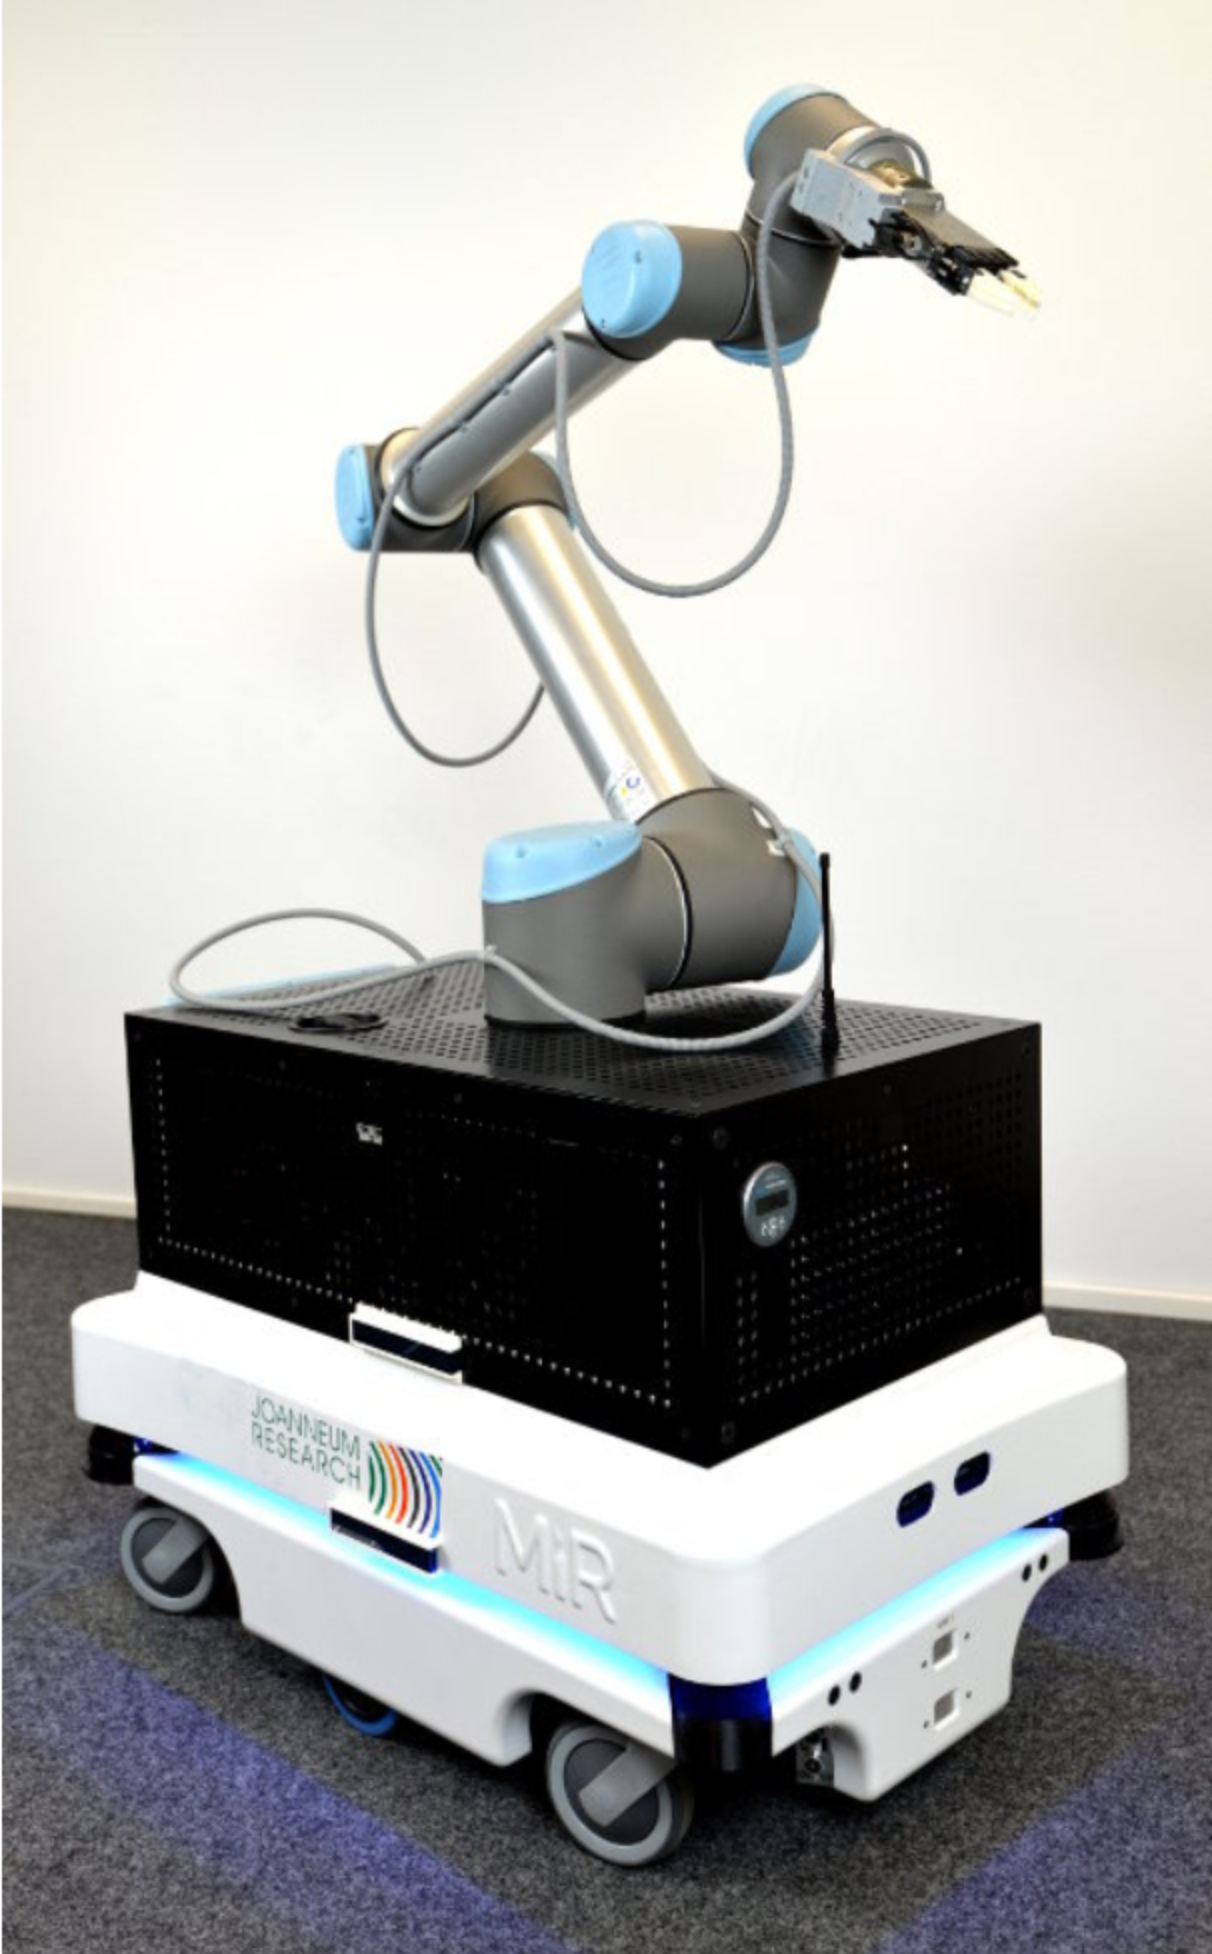
\includegraphics[scale=0.13]{Images/img_ch2/MobileManipulator.png}
    }
    \subfloat[KUKA-DLR manipulator.\label{fig:Manipulator}]{
        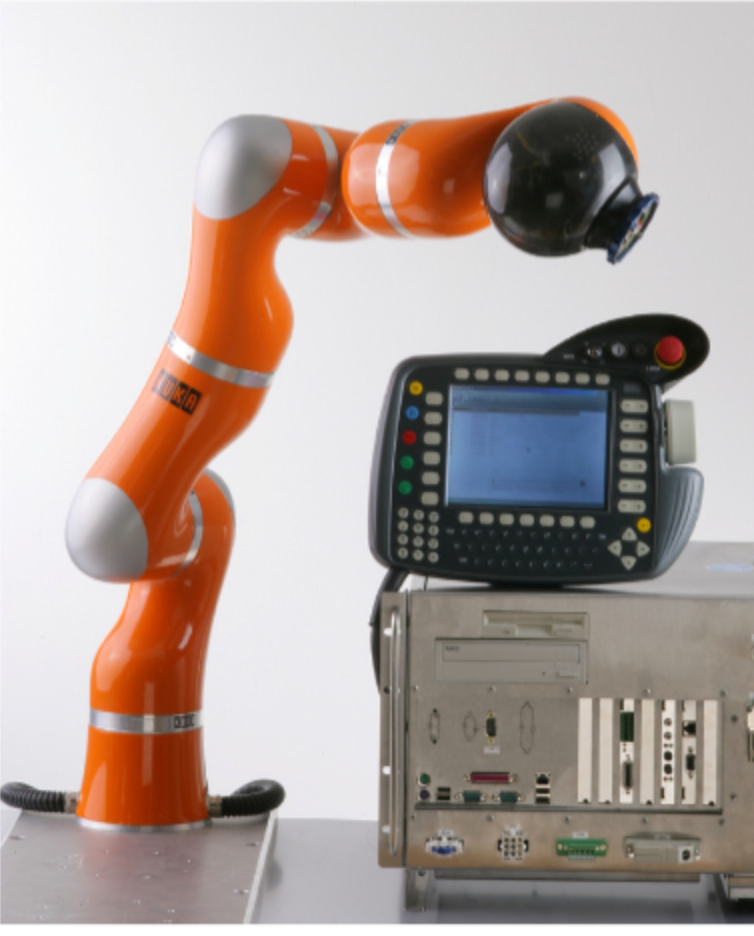
\includegraphics[scale=0.25]{Images/img_ch2/KUKA.png}
    }
    \caption[Examples of manipulators fixed and not.]{\cite{MOBILEMANIPULATOR}Mobile manipulator and \cite{KUKA}robotic arm}
    \label{fig:Manipulators}
\end{figure}

Raibert\cite{Raibert} and Todd\cite{Todd} give an extensive analysis of walking machines, while a clear definition of a legged robot can be found in \cite{Siciliano} or \cite{Legged}:

\begin{definition}\label{def:leggedSiciliano}
\cite{Siciliano}\textbf{Legged Robots} are made of multiple rigid bodies, interconnected by joints. Some of these bodies
form lower limbs, whose extremities (feet) periodically come in contact with the ground to realize locomotion
\end{definition}

\begin{definition}\label{def:legged}
\cite{Legged}\textbf{Legged Robots} use legs to move from one place to another. Legs provide an active suspension, so the motion of the main body of the robot can be largely decoupled from the terrain profile. With each step, a leg is temporarily
lifted off the ground, so that discontinuous terrain can be overcome as well, allowing locomotion in places out of reach otherwise.
\end{definition}

In the same article\cite{Legged}, legs in robotics are defined as:
\begin{definition}\label{def:leg}
\textbf{Legs} are usually articulated rigid bodies, assumed to contact the environment only with their end effector(EE). In most cases, this contact is unilateral,
meaning that the robot can push but not pull on contact surfaces
\end{definition}

In general, the design of legs is done to achieve walking locomotion (such as the quadrupeds in Fig.\ref{fig:WalkingRobots}). Using proper mechanical structures or innovative solutions\cite{climbing1}\cite{LEMUR3}\cite{SCARE_gripper}, also locomotion in walls and ceilings is possible, obtaining \textbf{climbing robots} (as the one in Fig.\ref{fig:LEMUR3}).

Finally, from Koyachi's works on multi-limbed robots, an explicit definition of limbed mechanism is given \cite{Koyachi}\cite{Koyachi2}\cite{Koyachi3}:

\begin{figure}[H]
    \centering
    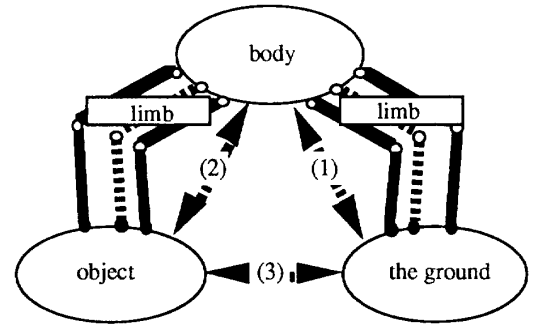
\includegraphics[width=0.5\textwidth]{Images/img_ch2/limb-mechanism.png}
    \caption{Scheme of Limb mechanism.\cite{Koyachi}}
    \label{fig:limb-mechanism}
\end{figure}

\begin{definition}\label{def:limb_mechanism1}
In robotics, a \textbf{Limb mechanism} is a link that connects the robot body with the environment. The objective with limb mechanism is to obtain the following motions (as in Fig.\ref{fig:limb-mechanism}) by moving each limb appropriately:
  \begin{itemize}
      \item (1) Relative motion between body and ground that
        causes locomotion of the robot.
      \item (2) Relative action between an object and a body that will
be used for handling and machining a small object.
      \item (3) Relative action between an object and base that will be
used for transferring and handling of an object, machining
of a large object.
  \end{itemize}
\end{definition}

From another publication of the same author\cite{Koyachi3}:  
\begin{definition}\label{def:limb_mechanism2}
In robotics, a \textbf{Limb mechanism} is a linkage integrating both locomotion and manipulation functions.
Ensuring the following features: 
\begin{itemize}
\item There is no clear boundary between walking and working spaces, and total efficiency increases because limbs can be used for walking or working according to the situation
\item Force generated by the hand increases and working space
is expanded because limbs can be coordinated and support
limbs can move the body
\item This mechanism can be compact and light because two
functions are integrated into one linkage.
\end{itemize}
\end{definition}
The working space, also called \textbf{workspace}, comes from manipulator theory, and it is defined as \cite{Siciliano}:
\begin{definition}\label{def:workspace}
The \textbf{workspace} is the region described by the origin of the end-effector frame when all the manipulator joints execute all possible motions.
\end{definition}

A formal definition of multi-limb robot cannot be found in literature, but an intuitive one can be deducted from the ones above: 

\begin{definition}\label{def:multilimb_robot}
A \textbf{multi-limb robot} is composed of a body and multiple limb mechanisms. Limb-end integrates both locomotion and manipulation through suction cups, magnets, adhesive materials, or miniature spine arrays \cite{Legged}\cite{Hirose1991}\cite{HorizontaltoVertical}\cite{passiveSpineTohoku}. In some cases, even \textbf{limb/leg}-wheeled \cite{AnymalDocThesis}\cite{WheelLegged}\cite{MAMMOTH}\cite{RollerWalker}\cite{HopperLegWheel} or multimodal mechanisms can be integrated\cite{GrieelUda}\cite{Armadillo}. If a transformable multimodal mechanism is used as limb-end, the robot can be defined \textbf{multi-modal}.
\end{definition}
SCAR-E in Fig.\ref{fig:SCARE} is a good example of a multi-limb robot, with its gripper(Fig.\ref{fig:SCARE_Gripper}) designed for climbing, manipulating, and walking.

To avoid any confusion, a final comment on robotic system classification has to be done, regarding the class of \textbf{Humanoid robots}\cite{HumanoidRobot}. These robots have a human-like physical appearance, with both manipulator and walking abilities, but the mechanical structures (arms and legs) used to achieve those tasks are different. Multi-limbed robots instead perform multiple tasks with the same limb structure. 

\begin{figure}[H]
    \centering
    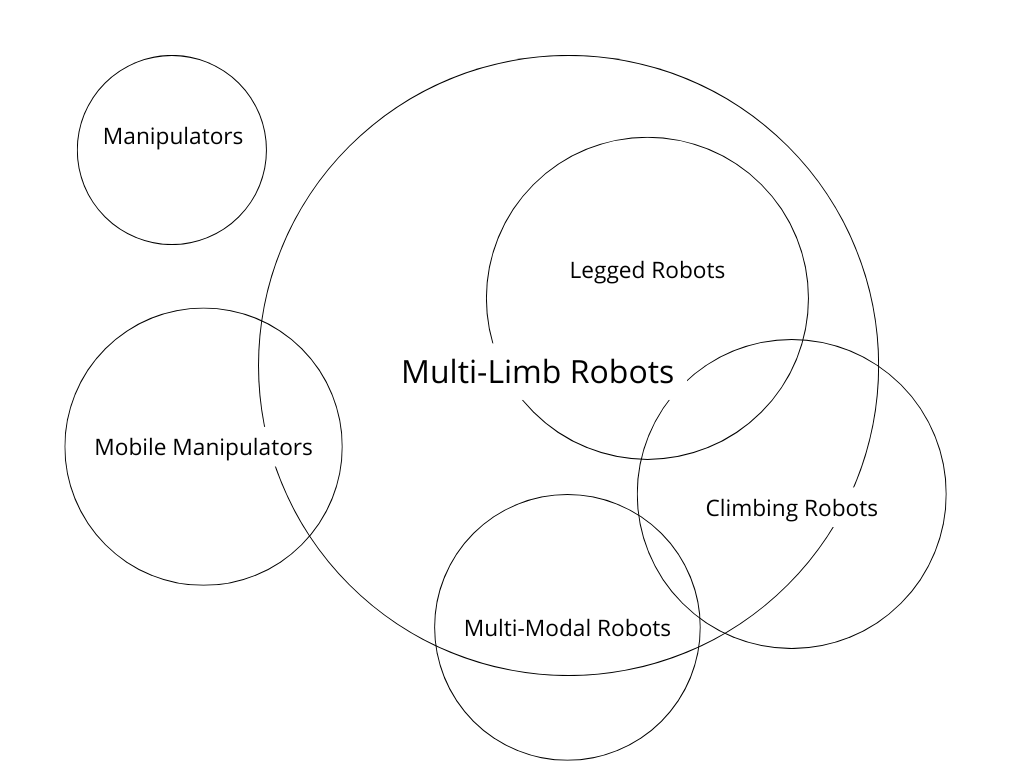
\includegraphics[width=0.8\textwidth]{Images/img_ch2/RobotClassificationVENN.png}
    \caption{Diagram of some robot classes}
    \label{fig:robotclasses}
\end{figure}

It is hard to identify a clear boundary among some of these classes of robots. Fig.\ref{fig:robotclasses} provides a diagram to summarize the concepts described in this section. 
This broad but mild classification highlights the reason why modeling and controlling limbed robots is not a simple task. 
A unique established theory doesn't exist. In the next chapters, first, state-of-the-art models of robot manipulators and legged robots are formalized, and then, some insights on possible solutions for limbed robots are given.

\section{Kinematic Model}
\label{sec:kinematic}

In mechanics, kinematics studies motion without considering its causes. When flexibility and softness are negligible in the system under analysis, rigid body theory is used.   

The rigid parts of the robot, also called links, are connected by joints, usually prismatic or revolute \cite{Siciliano}. The mobility of any robot is ensured by those joints, providing a single degree of freedom (DOF) each. 
An important concept when considering multi-body mechanics is the nature of the \textbf{kinematic chain}\cite{Siciliano}\cite{RoboticMechanics}. We classify it as: 
\begin{itemize}
\item \textbf{open kinematic chain} when only one sequence of links connects the mechanical chain's two ends (Fig.\ref{fig:openkin}). For example robot manipulators, but even dual-arm robots.
\item \textbf{closed kinematic chain} when the sequence
of links forms a loop(Fig.\ref{fig:closedkin}).
\end{itemize}. As a Parallelogram mechanism (used in construction vehicles), or legged robots, considering the "connection" between feet tip through a common ground \cite{RoboticMechanics}\cite{QuadrupedLocomotion}. 

\begin{figure}[H]
    \centering
    \subfloat[Open chain.\label{fig:openkin}]{
        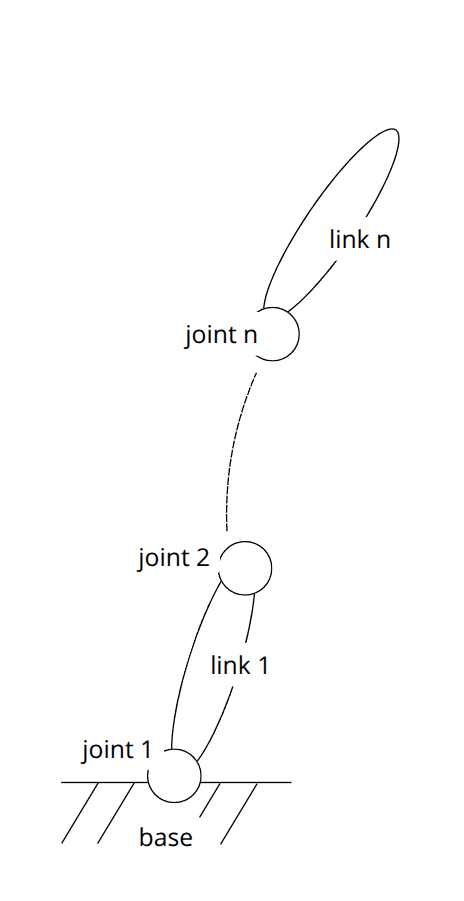
\includegraphics[scale=0.3]{Images/img_ch2/OpenKinChain.png}
    }
    \quad
    \subfloat[Closed chain.\label{fig:closedkin}]{
        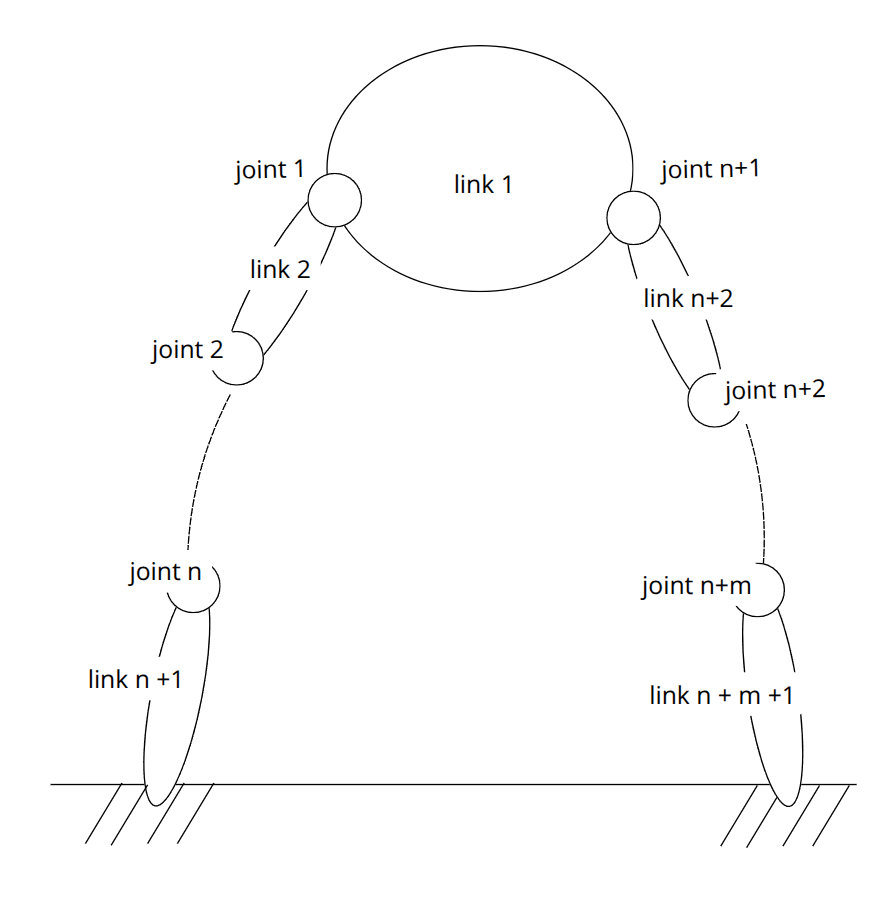
\includegraphics[scale=0.3]{Images/img_ch2/ClosedKinChain.png}
    }
    \caption[Scheme of possible kinematic chains]{Simple representation of open/closed kinematic chains.}
    \label{fig:quadtree2}
\end{figure}


In robotics, three main problems are considered: \textbf{forward}(FK), \textbf{inverse}(IK), and \textbf{differential kinematics} (DK). These are formally defined and solved for manipulators, legged, and multi-limb robots. 

\subsection{Forward Kinematic}
\label{sec:forward}
The role of FK is to derive the relationship between joint variables and the pose of a final link frame\cite{CorkeMATLAB}\cite{Siciliano}. 
The "final link" depends on the type of robot. 
For a manipulator, it is the end effector, which is the last element of the open chain, usually carrying a tool. 
In legged and multi-limb robots, the pose of all legs/limbs tips is important. 

Independently of the structure under analysis, the foundation of kinematics is the relationship between link frames. Each link is identified by an attached reference frame, and its pose is defined as the position and orientation of that frame \cite{Siciliano}\cite{RoboticMechanics}\cite{CorkeMATLAB}.
The choice of each link frame is not unique, the \textbf{Denavit-Hartenberg} (DH) convention \cite{DenavitHartenberg} provides a standard way to define it.

Collecting all variables of the n joints in a vector $\mathbf{q} \in \mathbb{R}^n$ (time dependency is omitted), the final result of FK is a homogenous 4x4 transformation matrix $\mathbf{T^0_f(\mathbf{q})}$, "0" identify the inertia frame, "f" the final frame in consideration. 
This matrix contains information about the position and orientation: 
\begin{equation}
\label{eq:homogeneus}
    \mathbf{T^0_f(\mathbf{q})} =
        \begin{bmatrix}
        \mathbf{R^0_f(\mathbf{q})} & \mathbf{^0p_f(\mathbf{q})} \\
        \mathbf{0}^{\top} & 1
        \end{bmatrix}
\end{equation}

Here, the dependency on joint configuration \textbf{q} is explicit, to clarify how FK is a function of joint configuration, for notation conciseness, sometimes it is omitted.
Furthermore, "0" is omitted in some cases, considering the inertial frame granted, 
$\mathbf{R^0_f} = \mathbf{R_f}$, $\mathbf{^0p_f} = \mathbf{p_f}$, and so on.
$\mathbf{T^0_f}$ is a powerful mathematical tool that not only contains information about the pose but also a matrix transformation to change the reference frame. If we consider the homogeneous coordinates ($\tilde{p} = \begin{bmatrix}
    \textbf{p} & 1
\end{bmatrix}^T$) of a generic point A in space, it holds:
\begin{equation}
\label{eq:pointTransform}
    \mathbf{\tilde{^0p_A}} = \mathbf{T^0_f} \cdot \mathbf{\tilde{^fp_A}} 
\end{equation}


Additionally, transformation matrix composition is as easy as a matrix product, and it can be chained.
\begin{equation}
\label{eq:chainTransform}
    \mathbf{T^0_f} = \mathbf{T^0_i} \cdot \mathbf{T^i_j} \cdot ... \cdot \mathbf{T^m_f}
\end{equation}

The drawback of using homogeneous transformation is the redundancy of $\mathbf{R^0_f}$ as orientation description. 
 Minimal or quai-minimal representations such as Euler angles or quaternion are often used \cite{Siciliano}.

In general, a pose in 3D space is described by 6 DOFs, 3 for rotation and 3 for orientation. In some cases, the task of the robotic structure requires less than 6 DOFs, and a task vector $\mathbf{x} \in \mathbb{R}^m$  is defined. The space in which the task is defined is called \textbf{operational/task space} (of dimension m), and it is always possible to derive a non-linear function, relating joint variables (in the so-called \textbf{joint space}) to this task vector: 
\begin{equation}
\label{eq:directKinematic}
    \mathbf{x} = \mathbf{k(q)}
\end{equation}

$\mathbf{x}$ collects position (\textbf{p}) and orientation (\textbf{$\phi$}) as: 
    $\mathbf{x} = \begin{bmatrix}
        \mathbf{p} & \mathbf{\phi}
    \end{bmatrix}^T $

A common minimal representation of orientation is the XYZ Euler angles also called Roll $\vartheta$, Pitch $\varphi$, Yaw $\psi$(RPY) (see Fig.\ref{fig:RPY}):
$\mathbf{\phi} = \begin{bmatrix}
        \vartheta &  \varphi &  \psi
    \end{bmatrix}^T$

\begin{figure}[H]
    \centering
    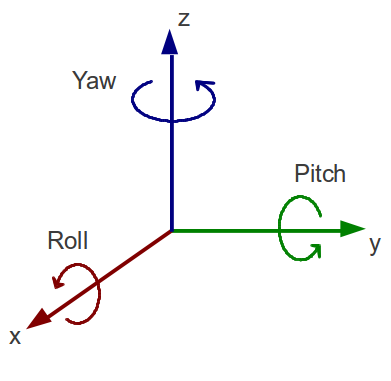
\includegraphics[width=0.3\textwidth]{Images/img_ch2/RPY.png}
    \caption{Roll Pitch Yaw angles}
    \label{fig:RPY}
\end{figure}

The explicit expression of the vectorial function $\mathbf{k(q)} \in \mathbb{R}^m$ is often derived by geometrical analysis of the robotic structure ($\mathbf{T^0_f}$ can also be computed in this way).

\begin{figure}[H]
    \centering
    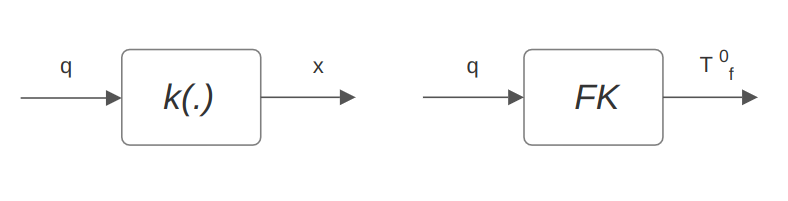
\includegraphics[width=0.8\textwidth]{Images/img_ch2/FKScheme.png}
    \caption{Block scheme of FK problem}
    \label{fig:FKScheme}
\end{figure}

Fig. \ref{fig:FKScheme} summarizes the kinematic problem and its resolution, Solving it is easy for an open kinematic chain robot, problems arise when the system presents closed chains.

The next part of this section presents techniques to solve FK for the robotics structure of interest.

\subsubsection{Manipulators and Single-Leg/Limb}
\label{sec:manipulatorFK}

\begin{figure}[H]
    \centering
    \subfloat[\cite{UR_DH_Parameters}UR DH frames.\label{fig:UR}]{
        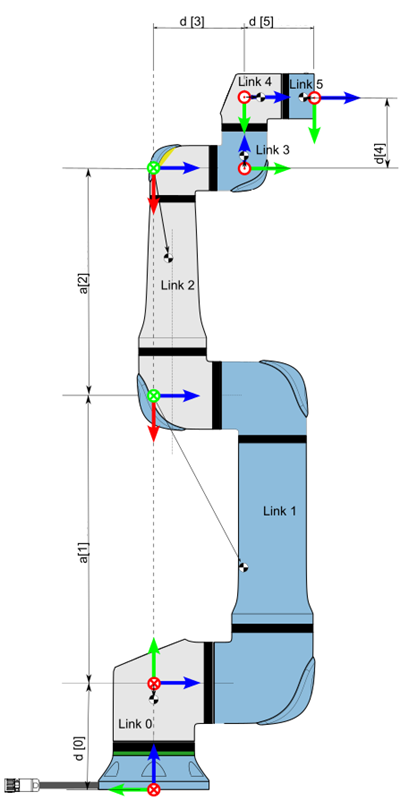
\includegraphics[scale=0.35]{Images/img_ch2/URKinematic.png}
    }
    \subfloat[\cite{Siciliano}Open kinematic chain frames.\label{fig:manipulatorFK}]{
        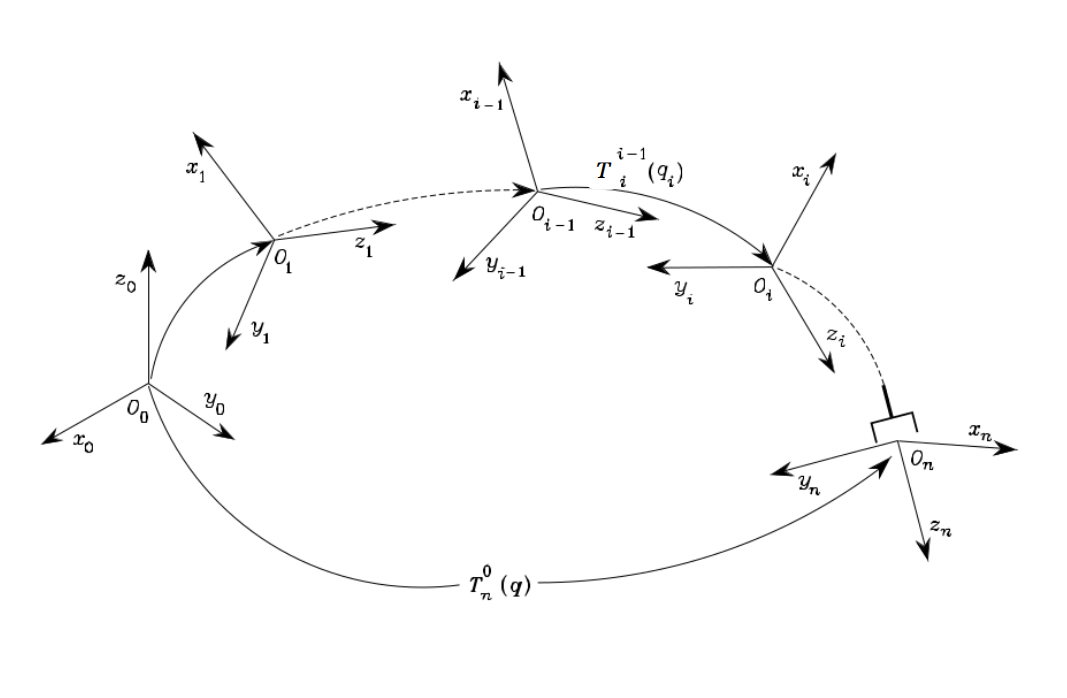
\includegraphics[scale=0.25]{Images/img_ch2/OpenChainKinFK.png}
    }
    \caption[forward kinematic in manipulators]{Example of DH Frames  in UR series manipulator(a), and scheme of open kinematic chain frames(b)}
    \label{fig:FKManipulator}
\end{figure}

In the context of \textbf{Robotic Manipulators}, the final frame (previously called \textbf{f}) is usually the final link frame (where a tool can be attached), defined as frame \textbf{n} (other times as end-effector frame \textbf{e}). 
Considering relation (\ref{eq:chainTransform}), for an open chain of n links, as the one in Fig.\ref{fig:manipulatorFK}, the resolution of FK with \textbf{homogeneous transformations} is straightforward:
\begin{equation}
\label{eq:FKManipulator}
    \mathbf{T^0_n(q)} = \mathbf{T^0_1(q_1)} \cdot \mathbf{T^1_2(q_2)} \dots \cdot \mathbf{T^{i-1}_{i}(q_i)} \dots \cdot \mathbf{T^{n-1}_n(q_n)}
\end{equation}

With $q_{i}$ defining the joint connecting links $i-1$ to $i$, It is straightforward that  $\mathbf{T^{i-1}_{i}(q)} = \mathbf{T^{i-1}_{i}(q_i)} $.

In principle, the choice of each link frame is arbitrary, nevertheless, respecting the DH convention (as in Fig.\ref{fig:UR}) brings some advantages:  
\begin{itemize}
    \item It is a standard convention, which avoids any ambiguity.
    \item $\mathbf{T^{i-1}_{i}(q_i)}$ $\forall i$ can be computed in a standard form from DH Parameters.
\end{itemize}

In simple cases, such as the manipulator in Fig.\ref{fig:ThreeLinkPlanar}, the pose of the final frame can be computed explicitly using \textbf{geometric considerations}. 

\begin{figure}[H]
    \centering
    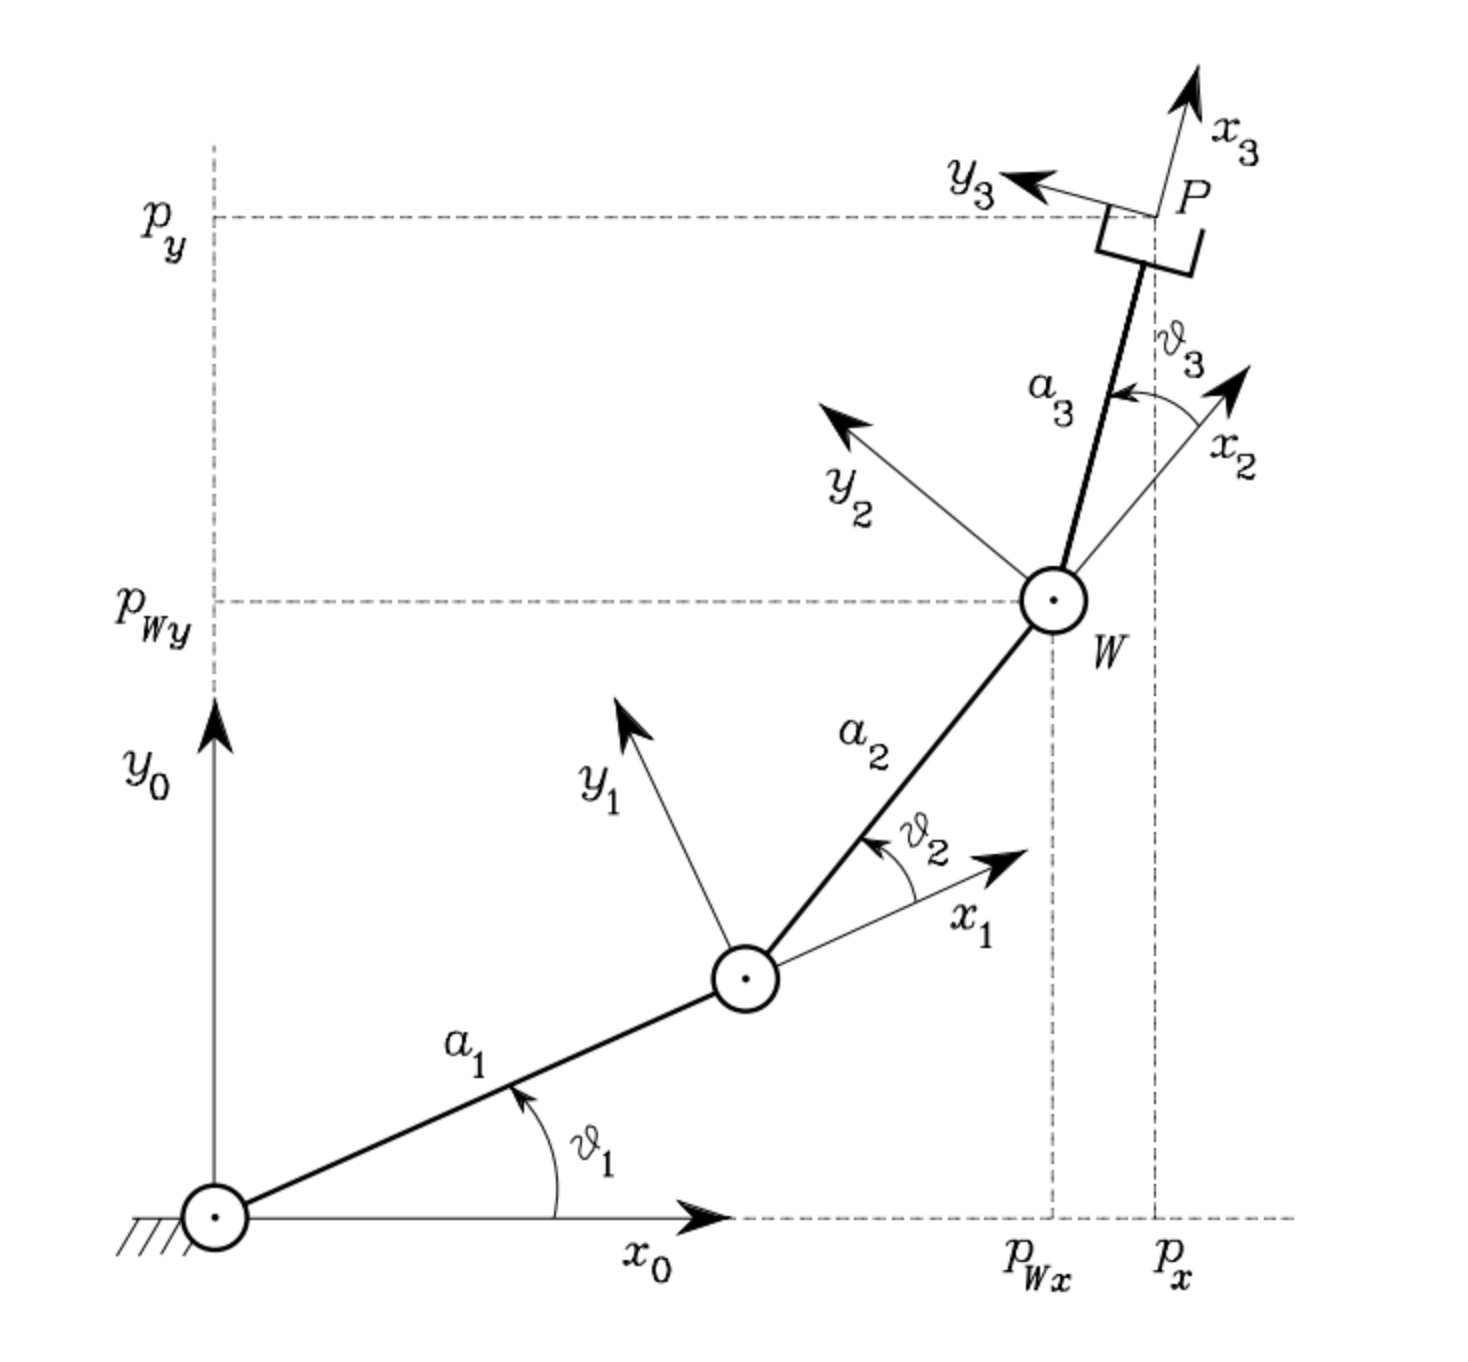
\includegraphics[width=0.6\textwidth]{Images/img_ch2/ThreeLinkPlanarArm.png}
    \caption{\cite{Siciliano}Three-link planar arm}
    \label{fig:ThreeLinkPlanar}
\end{figure}

The Three-link planar arm above provides useful insights into the meaning of \textbf{task space}. 
This mechanical structure allows planar motion in the XY plane. 
with reference to the symbols in the figure, $\mathbf{q} = \begin{bmatrix}
\vartheta_1 & \vartheta_2  & \vartheta_3 \end{bmatrix}^T$, $\mathbf{x} = \begin{bmatrix}
p_x & p_y  & \psi \end{bmatrix}^T$, where $p_x$, $p_y$ represents the EE position, while  $\psi = \vartheta_1 + \vartheta_2  + \vartheta_3 $ the EE orientation (as yaw angle). 
Deriving the expression of $\mathbf{T^{0}_{3}(q)}$ or $\mathbf{k(\cdot)} \in \mathbb{R}^3$ is not relevant here.

To introduce some commonly used reference frames, consider the following example. 
In Fig.\ref{fig:TITAN4Frames} below, the TITAN4 \cite{manipulatorTITAN4} is considered, with a fixed base. The inertial frame is the world frame \textbf{w}, \textbf{b} is a fixed frame attached to the base, frames from \textbf{0} to \textbf{n} identify robot links, and finally \textbf{e} is attached to the EE. 
Homogeneous transformation composition as in \ref{eq:FKManipulator} is used:
\begin{equation}
\label{eq:FKTITAN4}
    \mathbf{T^w_e(q)} = \mathbf{T^w_b} \cdot \mathbf{T^b_0}\cdot \mathbf{T^0_1(q_1)}  \dots \cdot \mathbf{T^{i-1}_{i}(q_i)} \dots \cdot \mathbf{T^{n-1}_n(q_n)}\cdot \mathbf{T^n_e}
\end{equation}
Defining the pose of the EE frame in the world inertial frame. 


\begin{figure}[H]
    \centering
    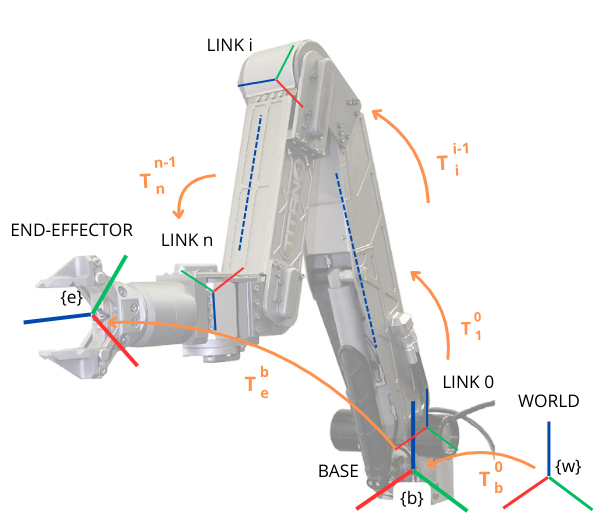
\includegraphics[width=0.7\textwidth]{Images/img_ch2/TITAN4.png}
    \caption{\cite{manipulatorTITAN4}Reference frames of fixed manipulator TITAN4}
    \label{fig:TITAN4Frames}
\end{figure}

These concepts can be extended to any open-chain structure, even to a stand-alone robotic leg/limb (as the ones defined in Def.\ref{def:leg} and  Def.\ref{def:limb_mechanism2}).

For example, the robotic leg in Fig.\ref{fig:KinematicLeg} has been described with the DH convention, to analyze the gait of a large-load-ratio six-legged robot \cite{LegDH}.
Here, the model considers the open kinematic chain from the leg root to the leg tip (as the final frame). 
With reference to Fig.\ref{fig:LegFrames}, denoting the frame attached to the leg root as \textbf{r}, and the one on the leg tip as \textbf{f}, it is possible to derive $\mathbf{T^r_f}$. Then, $\mathbf{T^w_r}$ is needed to obtain position and orientation in the inertial frame. This transformation matrix can be derived as $\mathbf{T^w_r} = \mathbf{T^w_b} \cdot \mathbf{T^b_r} $, where $\mathbf{T^w_b}$ denote the transformation from world inertial frame to the robot base, while $\mathbf{T^b_r}$ from robot base to limb root. It is just a matter of transformation composition. 

So, if the base pose is known ($\mathbf{T^w_b}$), it is possible to track the foot motion when the leg is above the ground. The same holds for any \textbf{limbs}, this modeling approach and classical manipulator FK theory can be used to plan manipulation tasks or limb motion. 

\begin{figure}[H]
    \centering
    \subfloat[Concept of 3 DOF robotic leg for walking.\label{fig:Leg}]{
        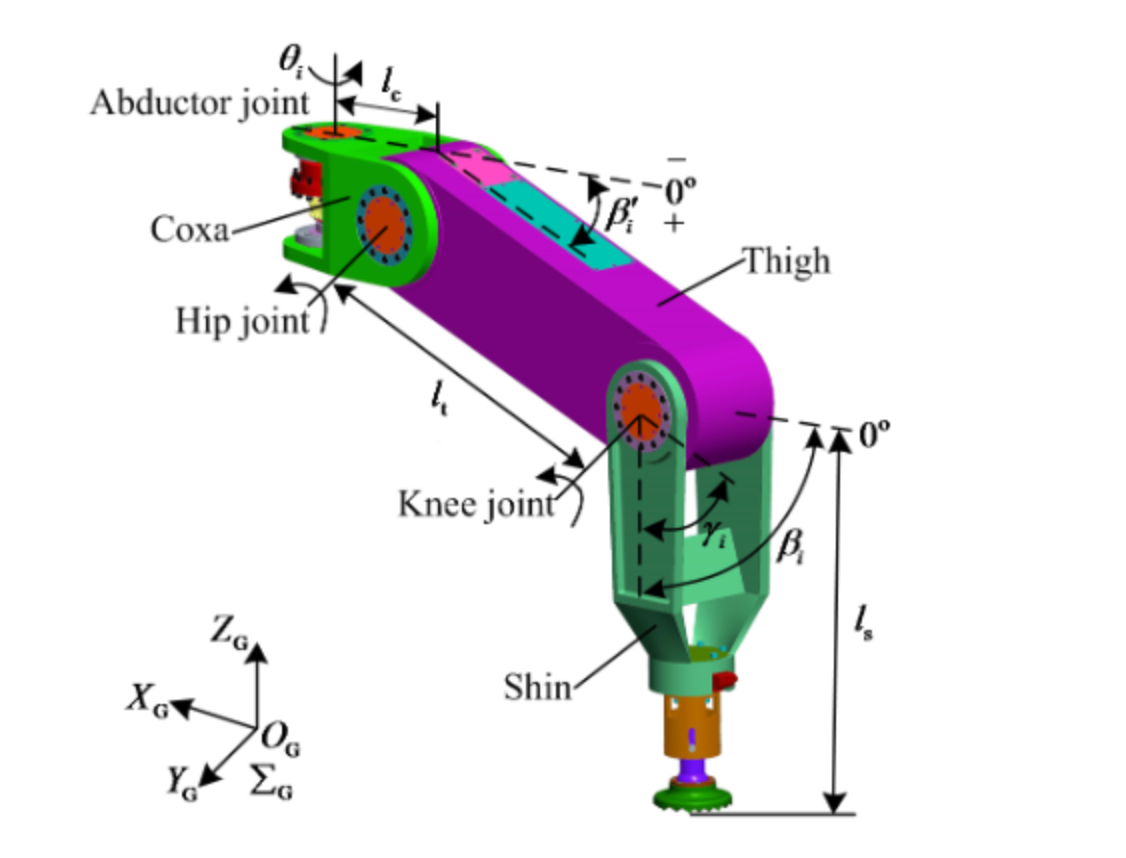
\includegraphics[scale=0.20]{Images/img_ch2/RoboticLeg.png}
    }
    \subfloat[DH frames for the same leg.\label{fig:LegDH}]{
        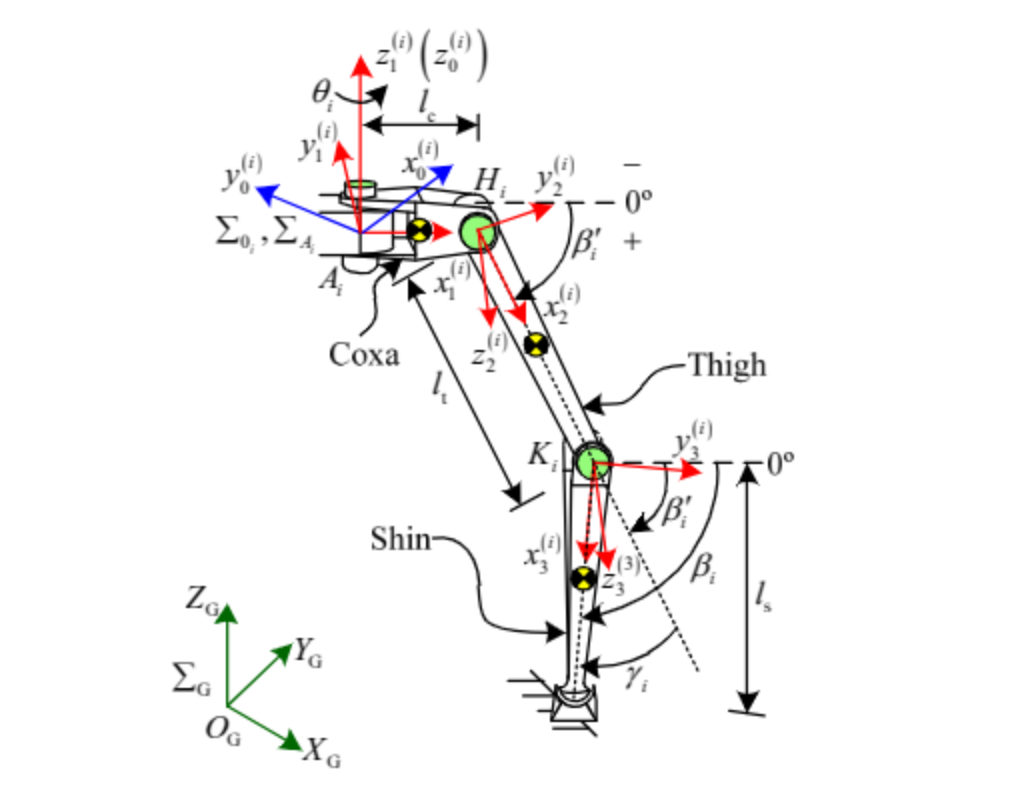
\includegraphics[scale=0.25]{Images/img_ch2/RoboticLegDH.png}
    }
    \caption[Open Kinematic chain Leg DH]{\cite{LegDH} Leg design and DH frames as open kinematic chain}
    \label{fig:KinematicLeg}
\end{figure}

\begin{figure}[H]
    \centering
    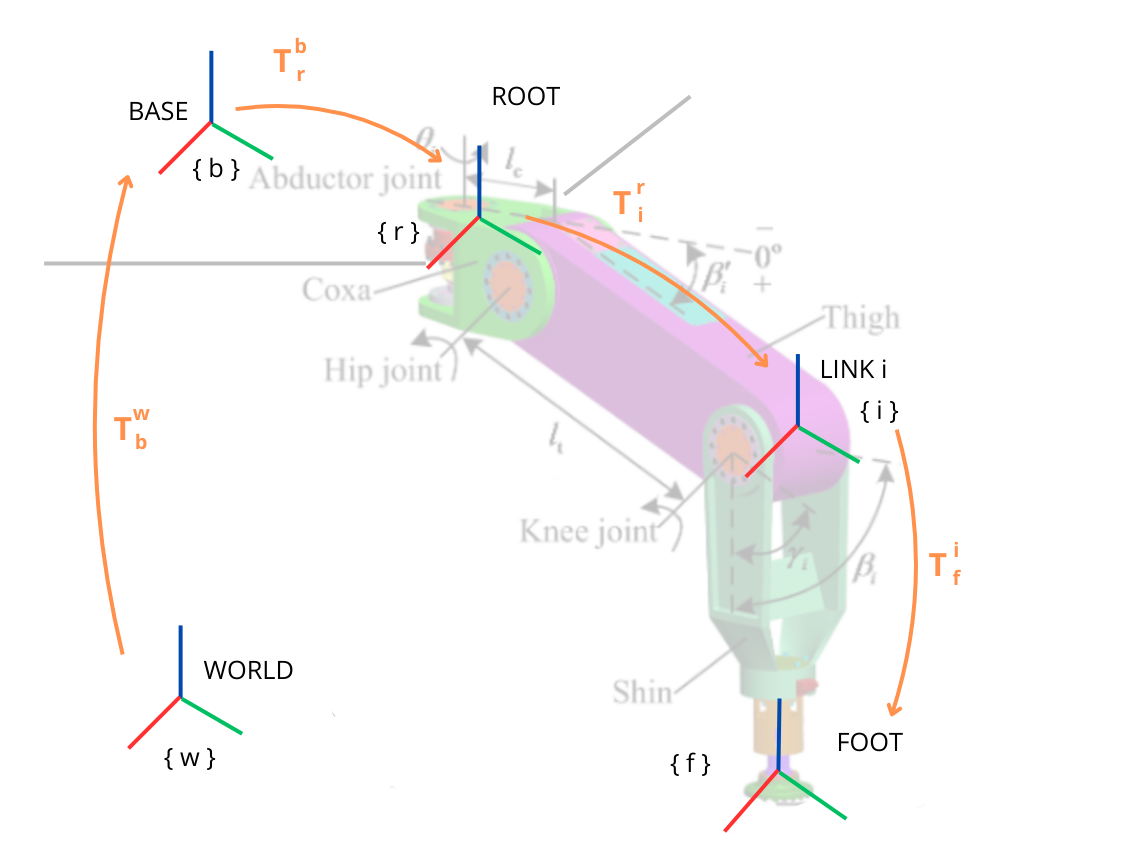
\includegraphics[width=0.7\textwidth]{Images/img_ch2/LIMB_FRAMES.png}
    \caption{Reference frames of single leg}
    \label{fig:LegFrames}
\end{figure}

It is important to notice the difference between the fixed manipulator and leg/limb kinematic. While in the first $\mathbf{T^w_b}$ is fixed and usually known, in the latter, the base is in motion, so $\mathbf{T^w_b}$ changes over time. The same holds when a mobile manipulator kinematic is analyzed. 
In the next section, this difference is further analyzed to define the kinematic of legged robots. 


\subsubsection{Legged Robots, Walking Machines}
\label{sec:leggedFK}

First, some terminology and symbols for walking robots is introduced. 
\begin{itemize}
    \setlength\itemsep{-0.7em} 
    \item \textbf{Base}: mobile base of the legged/limbed robot, \textbf{body} and \textbf{torso} are synonyms.
    \item \textbf{Gait}: walking pattern
    \item \textbf{Gait cycle}: Period between two rising phases of the same leg during gait.
    \item \textbf{Stance phase}: phase in which the leg is in contact 
    \item \textbf{Swing phase}: phase in which the leg is not in contact, changing the contact point 
\end{itemize} 

Expanding the notation used in the previous chapter to describe a single limb open chain model, it is possible to define all $\textbf{N}$ legs kinematics. 
Denoting the limb index with $j = 1,..,N$ and the joint with $i$, $q_{j,i}$ identify joint $i$ of limb $j$. Usually, all legs have the same number of joints, but in general, $n_j$ is the number of joints of leg $j$, and $n = {\sum_j{n_j}}$ is the overall number of joints.
$\mathbf{q_j} \in \mathbb{R}^{n_{j}}$ is the vector collecting all joint variables for leg $j$, while $\mathbf{q} \in \mathbb{R}^n$is the vector of all legs joint variables (system actuated DOFs). 
The relevant frame when analyzing the whole kinematic are \textbf{b}, \textbf{w}, {$\mathbf{r_j}$}, {$\mathbf{f_j}$}, {$\mathbf{j_i}$} (denoting link $i$ of leg $j$).
commonly, \textbf{b} is located in the base center of mass (CoM), {$\mathbf{r_j}$} is rigidly attached to the base and identify the point where the first joint of the leg is attached. The definition of {$\mathbf{j_i}$} instead is arbitrary, DH convention can be used, while {$\mathbf{f_j}$} identify the foot tip, where the leg contacts the ground.  
Fig.\ref{fig:LeggedCoordinates} gives a graphical representation of this model. A quadruped is represented, but the theory is generalizable for any N-legged robot. 

\begin{figure}[H]
    \centering
    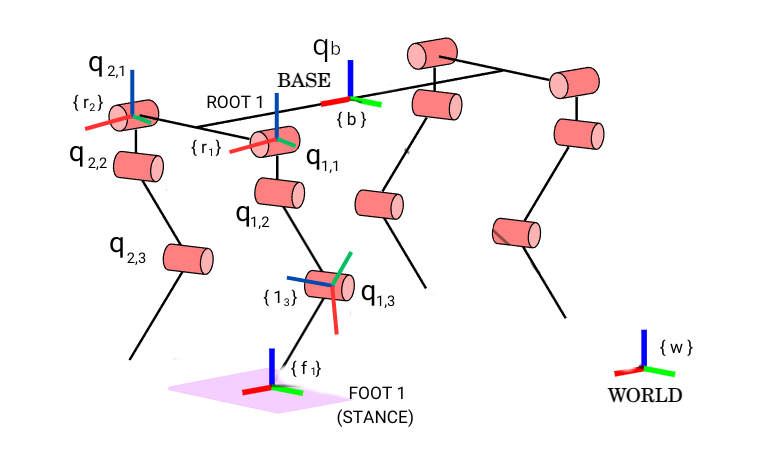
\includegraphics[width=0.9\textwidth]{Images/img_ch2/LeggedCoordinates.png}
    \caption{\cite{FloatingBase1} Quadruped kinematic model}
    \label{fig:LeggedCoordinates}
\end{figure}

As introduced in the previous section, in legged robots the base moves in the world frame. In legged locomotion \cite{QuadrupedLocomotion}, there are two main problems: 
\begin{enumerate}
    \setlength\itemsep{-0.7em} 
    \item Feet positioning to perform the gait
    \item Base positioning to maintain stability 
\end{enumerate}
These two problems introduce two different kinematic objectives, discussed briefly here.

\textbf{Problem 1: Feet positioning}

Estimation of the base pose in
the world is known as \textbf{localization} problem\cite{ProbabilisticRobotics}\cite{LeggedLocalization}(present in any mobile robot), which is outside of the scope of this research.
Furthermore, motion is achieved by a discrete placement of feet along the path. The problem of \textbf{path planning}\cite{LeggedPlanning1} requires the definition of each foot stance position. 
This concept is discussed in \ref{sec:leggedControl}, for now, it is important to anticipate that to achieve legged locomotion, foot position is usually computed in the base frame \textbf{b}. 

For those reasons, this forward kinematic problem consists of deriving the pose of each foot tip $\mathbf{f_j}$ in the base frame \textbf{b} ($\mathbf{T^b_{f_j}}$) (sometimes in the world \textbf{w} frame,$\mathbf{T^w_{f_j}}$).  
Knowing the pose of the base \textbf{b} in the world \textbf{w} ($\mathbf{T^w_b}$), and all joint variables $\mathbf{q_j}$ of each leg j.


Under this hypothesis, the \textbf{floating base} model \cite{FloatingBase2}\cite{LeggedThesis} is used. The base pose introduce 6 additional DOFs in 3D, $\mathbf{q_b} = \begin{bmatrix}
        x_b & y_b & z_b & \vartheta_b & \varphi_b & \psi_b
    \end{bmatrix}^T $ 
included in the system DOFs $\mathbf{q_{tot}} = \begin{bmatrix}
        \mathbf{q} & \mathbf{q_b}
    \end{bmatrix}^T \in \mathbb{R}^{n+6}$.
$\mathbf{q_b}$ affect the system state but there isn't any dedicated actuator, so they are considered as unactuated virtual DOFs (see Fig.\ref{fig:FloatingBase}).  

\begin{figure}[H]
    \centering
    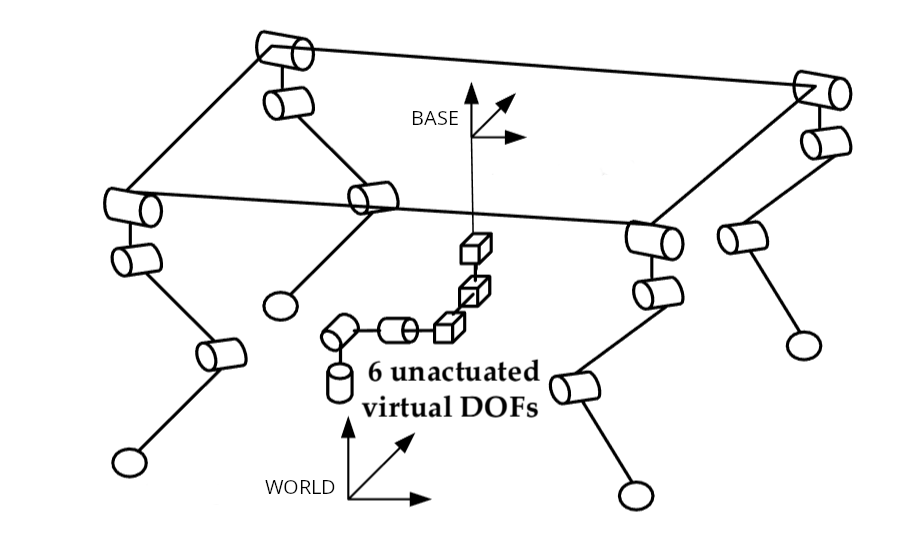
\includegraphics[width=0.6\textwidth]{Images/img_ch2/FloatingBase_2.png}
    \caption{Floating base model}
    \label{fig:FloatingBase}
\end{figure}

Refering to Fig.\ref{fig:FramesLegged}, to derive $\mathbf{T^b_{f_j}}$ an equation similar to \ref{eq:FKTITAN4} is used: 
\begin{equation}
\label{eq:FKLEG}
    \mathbf{T^b_{f_j}(q_j)} = \mathbf{T^b_r} \cdot \mathbf{T^r_{j_0}}\cdot \mathbf{T^{j_0}_{j_1}(q_{j,1})}  \dots \cdot \mathbf{T^{j_{i-1}}_{j_i}(q_{j,i})} \dots \cdot \mathbf{T^{j_{{n_j}-1}}_{j_{n_j}}(q_{j,{n_j}})}\cdot \mathbf{T^{j_{n_j}}_{f_j}}
    , \forall j=1,...,N
\end{equation}

If instead the foot position in the world frame is needed, the floating base DOFs are used
\begin{equation}
\label{eq:FKLEG}
    \mathbf{T^w_{f_j}(q_j, q_b)} = \mathbf{T^w_b(q_b)} \cdot \mathbf{T^b_{f_j}(q_j)}
    , \forall j=1,...,N
\end{equation}

\begin{figure}[H]
    \centering
    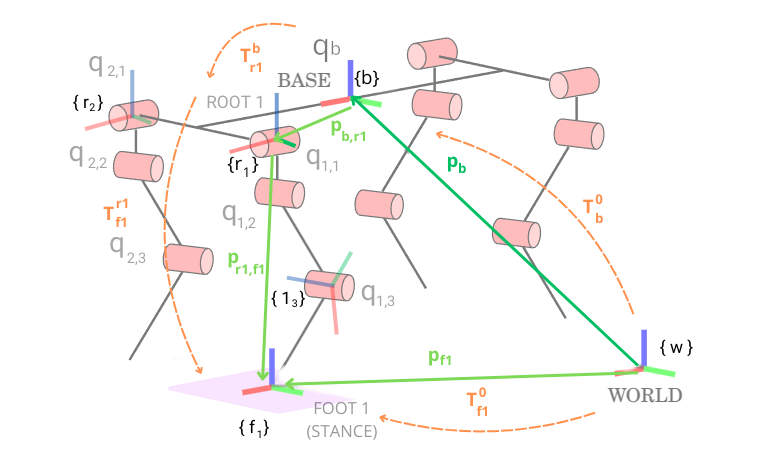
\includegraphics[width=1.0\textwidth]{Images/img_ch2/FramesLegged.png}
    \caption{Floating base kinematic position vectors}
    \label{fig:FramesLegged}
\end{figure}


\textbf{Problem 2: Base positioning}

In a legged machine, stability is a crucial aspect, explored in detail in \ref{ch:chapter_three}. For now, take for granted that to maintain the base stable, the base CoM is positioned in a specific region from the stance feet contact points. For this reason, it is important to describe the pose of the base from each foot contact point frame $\mathbf{T^{f_j}_b}$.

This forward kinematic problem consists of the derivation of the base pose \textbf{b} respect each contact leg foot $\mathbf{f_j}$ ($\mathbf{T^{f_j}_b}, \forall j \in J_c$), given the vector of leg $j$ DOFs $\mathbf{q_j}$.
Where $J_c$ defines the set of indices of legs in contact with the ground.

The kinematic model of each contact leg $j \in J_c$ is redefined for this purpose from the foot tip to the leg root as in Fig.\ref{fig:LegReversedKinModel}. 
Contact with the ground is assumed to take place such that the ground can exert only a “pushing” force on each leg but no moment. Thus, while we can model the contact between leg and ground as a spherical joint, care must be
taken so that no pulls of the ground on the leg are required for a given gait\cite{RoboticMechanics}
(The above assumption excludes climbing and complex multi-limb robot structures).

In this model, each contact foot frame $\mathbf{f_j}$ is attached to the foot tip and considered aligned with the ground in the xy plane. The spherical joint models the ground interaction and is represented by 3 rotational DOFs ($q_{j,1}, q_{j,2}, q_{j,3}$) of virtual unactuated joint variables (as for the floating base). 
The derivation of $\mathbf{T^{f_j}_b}$ is just a matter of homogeneous transformation composition as already described in depth:
\begin{equation}
\label{eq:FKLEG2}
    \mathbf{T^{f_j}_b(q_j)} = \mathbf{T^{f_j}_{j_1}(q_{j,1})} \cdot \mathbf{T^{j_1}_{j_2}(q_{j,2})} \cdot \cdot \mathbf{T^{j_{i-1}}_{j_i}(q_{j,i})} \dots \cdot \mathbf{T^{j_{n_{j}-1}}_{j_{n_{j}}}(q_{j,n})}\cdot \mathbf{T^{j_{n_{j}}}_{r_j}}\cdot \mathbf{T^{r_j}_b}
    , \forall j \in J_c
\end{equation}

\begin{figure}[H]
    \centering
    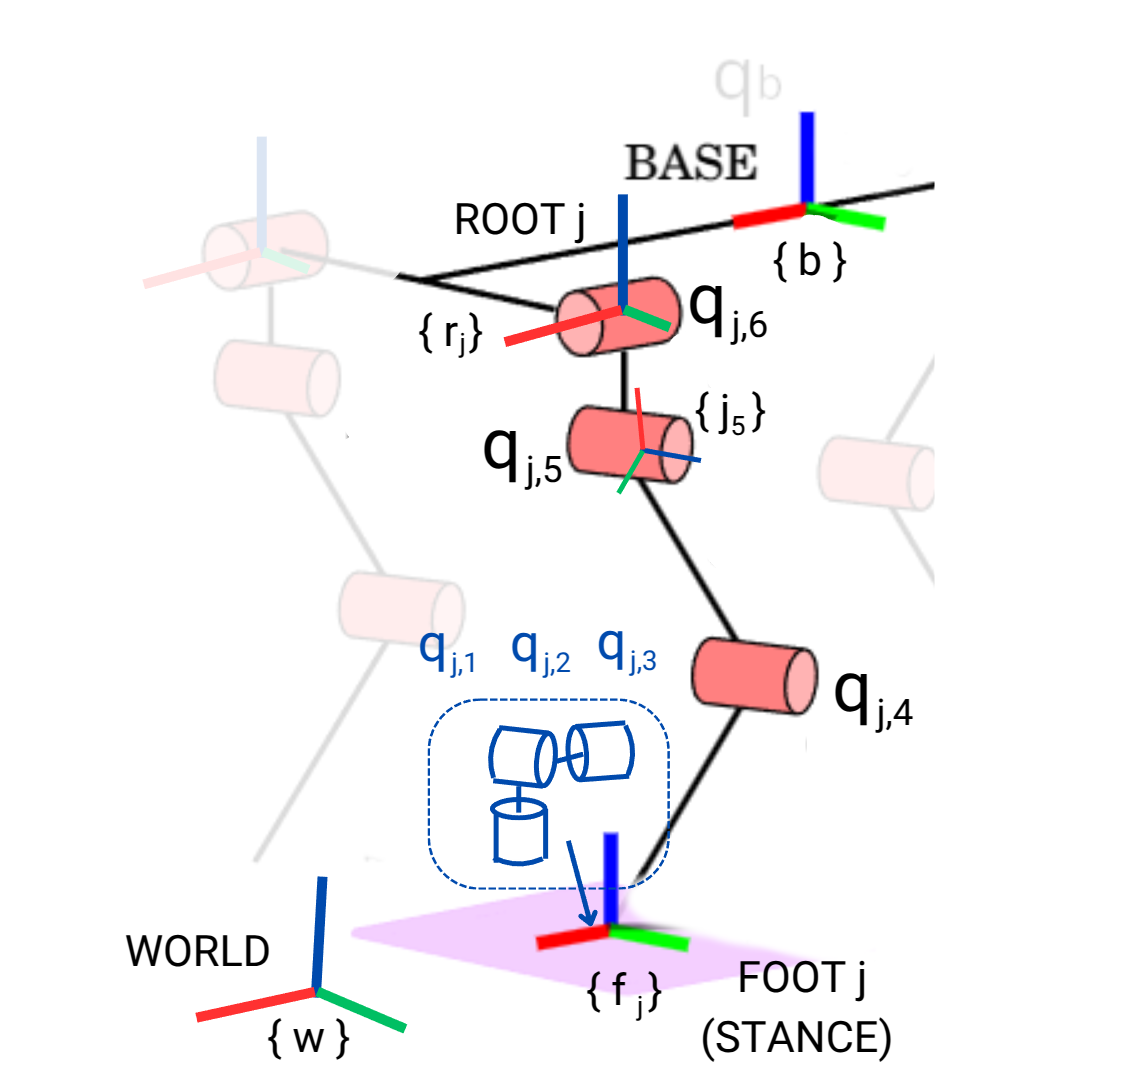
\includegraphics[width=0.6\textwidth]{Images/img_ch2/LegModeltiproot.png}
    \caption{Kinematic model of stance leg from foot tip to leg root}
    \label{fig:LegReversedKinModel}
\end{figure}

\subsubsection{Limbed Robots, Multipurpose Machines}
\label{sec:limbedFK}
From some limbed robots described in chapter \ref{ch:chapter_one}, the multifunctional aspect is clear.  
Those robots can move with walking locomotion, but also climbing, hybrid legged-wheeled driving, and even manipulate objects in the meantime\cite{SCAR-E}\cite{Koyachi}\cite{WheelLeggedStabilityOPT}. 
As for the kinematic modeling of walking machines defined in the previous section, different problems have to be solved. In general, we are interested in: 
\begin{itemize}
    \setlength\itemsep{-0.7em} 
    \item All limbs-end position respect base (or world) 
    \item Base pose respect limb-end 
\end{itemize}

The kinematic model for a generic multi-limb robot is as the one in Fig.\ref{fig:MultiLimbKin}.
The frames have the same meaning as for walking robots, except for the last frame referred to as $\mathbf{e_j}$. As for manipulators, any manipulation or locomotion "tool" can be attached to each limb's end frame (spine gripper, magnetic gripper, manufacturing tool, wheel, and so on...). 

\begin{figure}[H]
    \centering
    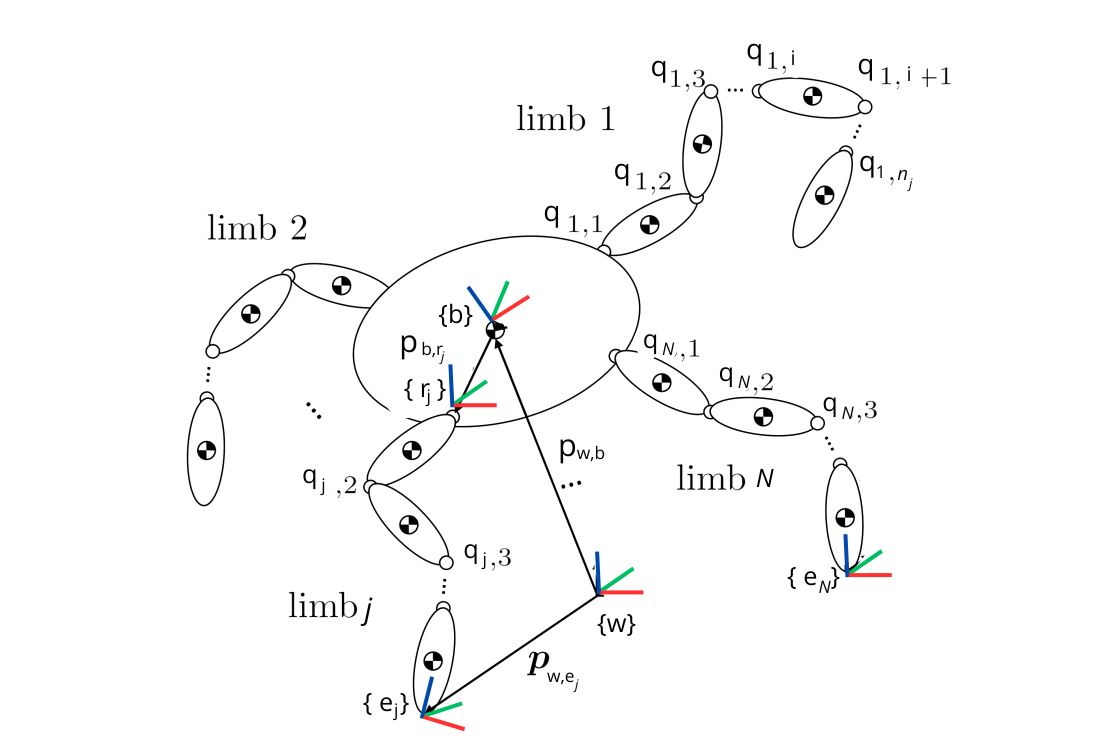
\includegraphics[width=0.85\textwidth]{Images/img_ch2/MultiLimbKin.png}
    \caption{\cite{Ribeiro2023reaction} model of multi-limb robot}
    \label{fig:MultiLimbKin}
\end{figure}

To solve the two main forward kinematic problems listed above, the same resolution as in equation \ref{eq:FKLEG2} (limb-end to base)and \ref{eq:FKLEG} (base to limb-end) can be applied. 


\newpage
Figure \ref{fig:FkAll} below summarizes the different robots' FK problems described here.
\begin{figure}[H]
    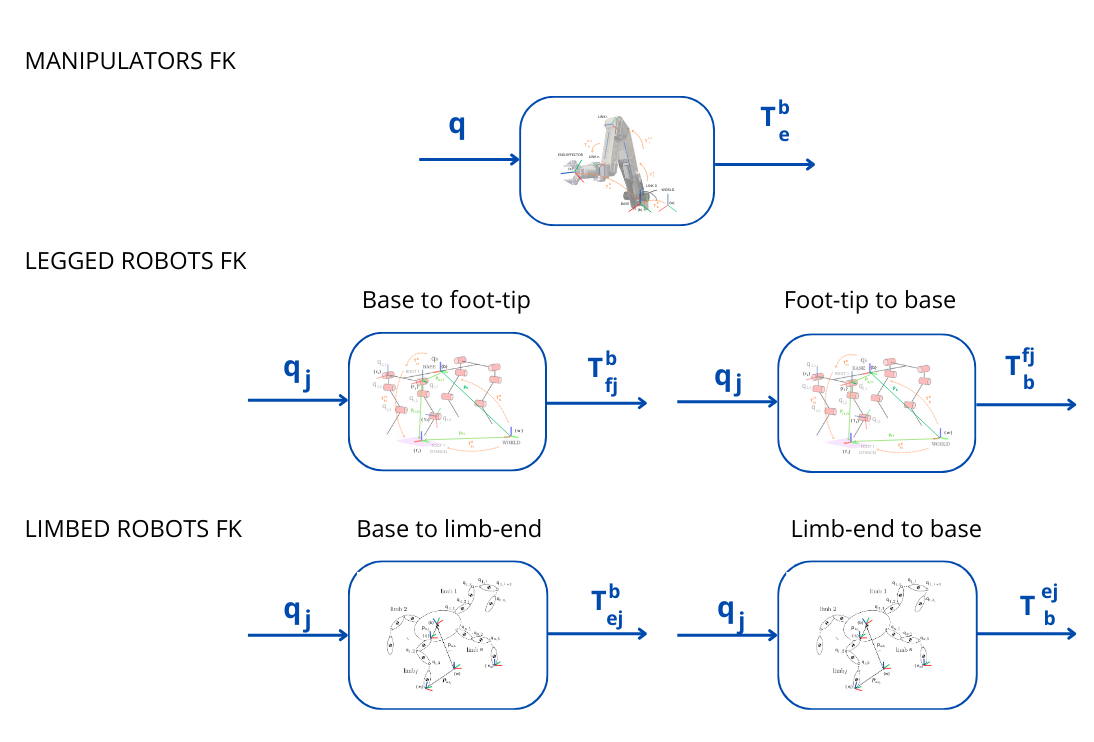
\includegraphics[width=1.1\textwidth, inner]
    {Images/img_ch2/FK_ALL.png}
    \caption{Scheme of FK problem for different robots}
    \label{fig:FkAll}
\end{figure}

With a standard procedure, the homogeneous transformation matrix is a way to represent the "final" frame pose. From that matrix, it is possible to extract the explicit FK equation $k(\cdot)$ in the task space. Alternatively, geometric analysis is always possible, but there isn't a standard formulation procedure.   

\subsection{Inverse Kinematic}
\label{sec:inverse}
As the name suggests, IK solves the Inverse problem of FK, going from the final frame pose (or task space) to the joint space \cite{Siciliano}\cite{RoboticMechanics}(as represented in Fig.\ref{fig:IKScheme}). 
From \cite{Siciliano}, in the context of \textbf{Manipulators}:
\textit{"The inverse kinematics problem consists of
the determination of the joint variables corresponding to a given end-effector position and orientation. The solution to this problem is of fundamental importance to transform the motion specifications, assigned to the end-effector in the operational space, into the corresponding joint space motions that allow execution of the desired motion"}.
So, in this formulation for different robotic structures, the "end-effector" could be the mobile base of the legged/limbed robot or the limb/leg end, depending on the task to execute.
\begin{figure}[H]
    \centering
    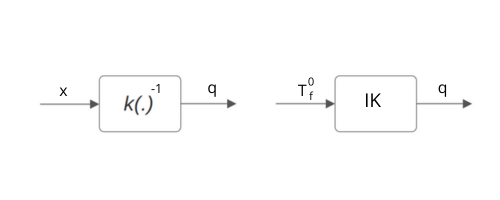
\includegraphics[width=0.7\textwidth]
    {Images/img_ch2/IKScheme.png}
    \caption{Scheme of general IK problems}
    \label{fig:IKScheme}
\end{figure}

Figure \ref{fig:IkAll} tries to summarize the IK problem for different robots with a simple scheme.
\begin{figure}[H]
%\hspace{-2cm} 
    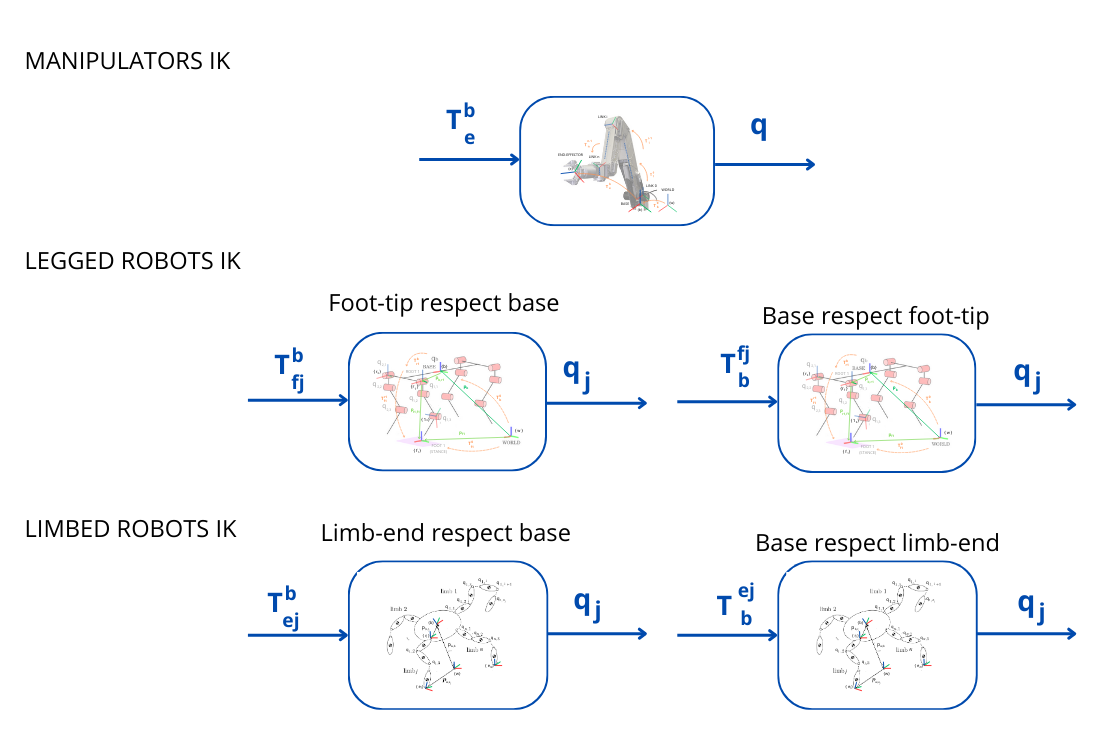
\includegraphics[width=1.1\textwidth, inner]
    {Images/img_ch2/IK_ALL.png}
    \caption{Scheme of FK problem for different robots}
    \label{fig:IkAll}
\end{figure}

\newpage
While FK has always one (and only one) solution, IK can have one, multiple (even infinite), or no solutions.

From the definition of workspace \ref{def:workspace}, it is clear that if a pose outside of it is chosen, IK cannot be solved. Due to mechanical constraints, link collisions, or design choice, the joint space $\mathbf{q} \in \mathbb{R}^n$ is an ideal space. The counter-image of the workspace is a subspace of the joint space, this can be defined as constrained joint space $\mathbf{\bar{q}} \subseteq \mathbf{q}$.
For example, for a single revolute joint mechanism, the joint space is $\mathbf{q} \in \mathbb{R}$, but if it can move only in between $-\pi$, $\pi$, then the constrained joint space is $\mathbf{\bar{q}} \in [-\pi, \pi]$.

There isn't a standard way to solve IK, some techniques are: 
\begin{itemize}
\item \textbf{FK algebraic inversion}:\newline
It consists of deriving the FK solution and inverting it.
But, whenever revolute joints are involved, it is clear that trigonometric functions of the joint variables appear in FK, not invertible in $\mathbf{\bar{q}}$.
Then, to invert it, assumptions on the constrained joint space domain are needed. Depending on the domain restriction, different solutions are found.
Even when a solution exists, finding a closed-form IK solution is hard and sometimes not possible. 
Having a closed-form solution makes computation faster and more reliable, expressed as: 
\begin{equation}
\label{eq:IK}
    \mathbf{q} = f_{IK}(\mathbf{x_f})
\end{equation}
Where $\mathbf{x_f}$ denotes the final frame task space vector.
When it is not possible, numerical methods are used.
\item \textbf{Numerical methods}:\newline
To solve non-linear equations, numerical methods such as Newton-Raphson\cite{ModernRobotics} are often used in robotics.
\item \textbf{Inverse differential kinematics}:\newline
This solution depends on the differential kinematic formulation, which will be discussed in section\ref{sec:differential}. For IK solution, once an explicit velocity relation is established between joint space and final frame velocity (goal of DK), it is inverted and integrated. 
\end{itemize}

Next, an overview of the IK problem for the robotics structure of interest is done. However, due to the absence of a standard method, the details of the resolution are not addressed here. 

\subsubsection{Manipulators and Single-Leg/Limb}
\label{sec:manipulatorIK}
The problem of IK for manipulators has already been introduced, formally: \\
\textit{Given a desired end-effector pose $\mathbf{T^0_e}$ ($\mathbf{T^w_e}$),or as $\mathbf{x}$, derive the joint configuration $\mathbf{q}$ to reach it.}



Again, as for FK, the same approaches can be used for single legs/limbs modeled from the base root attachment to the tip/end.
In that case, the problem is formulated as follows:\newline 
\textit{Given a desired limb $j$-end/leg $j$-tip  pose $\mathbf{T^b_{f_j/e_j}}$ ($\mathbf{T^w_{f_j/e_j}}$),or as $\mathbf{x_{f_j/e_j}}$, derive the joint configuration $\mathbf{q_j}$ to reach it.}

The IK problems described above are represented in Fig.\ref{fig:ArmLegIK}.
\begin{figure}[H]
    \centering
    \subfloat[\label{fig:ArmIK}]{
        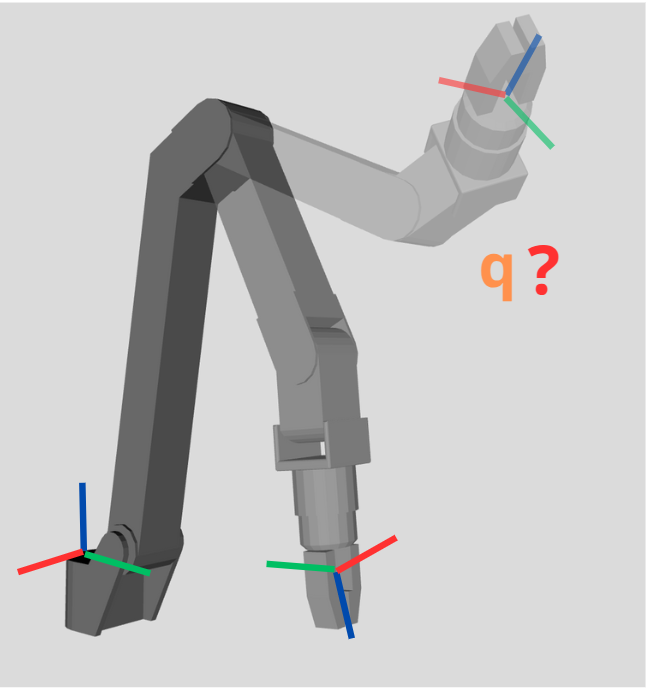
\includegraphics[scale=0.25]{Images/img_ch2/ArmIK.png}
    }
    \subfloat[\label{fig:LegIK}]{
        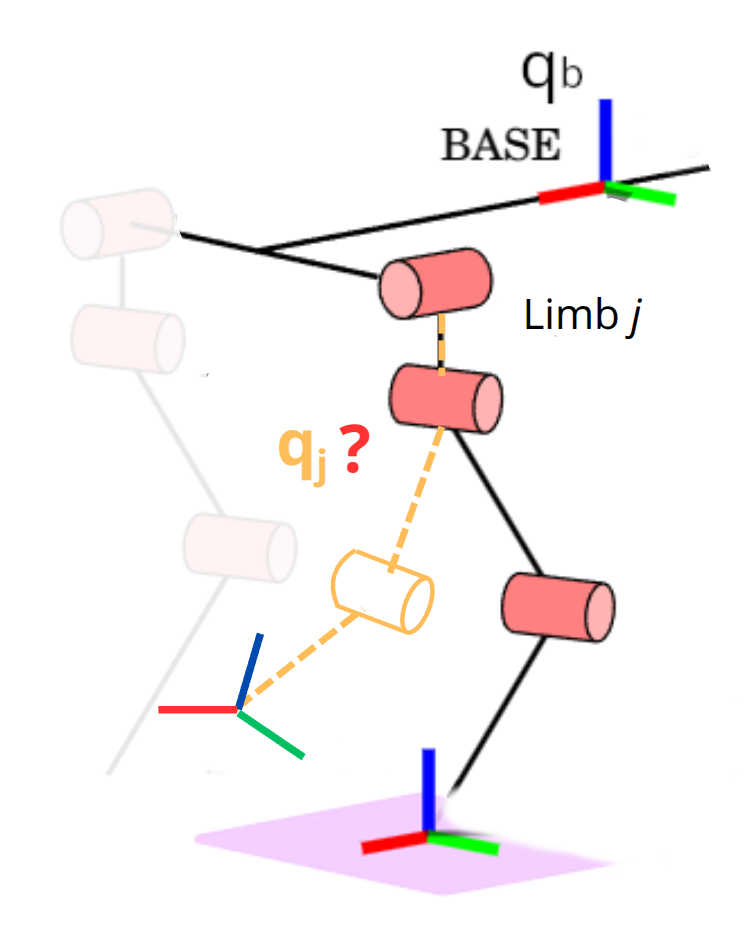
\includegraphics[scale=0.20]{Images/img_ch2/LegIK.png}
    }
    \caption[Leg/Limb and Arm IK]{IK problem for Manipulators (a) and single leg/limb (b)}
    \label{fig:ArmLegIK}
\end{figure}

The resolution of the IK described above is needed to plan any arm/limb manipulation or single leg/limb step. A different approach is used when positioning a legged/limb robot base. 
The definition of this IK problem is described in the next part. 

\subsubsection{Legged/Limbed Robots Base}
\label{sec:leggedLimbedIK}
The representation in Figure \ref{fig:IkAll} of IK for legged/limbed robots base is not complete. 
In fact, when dealing with base motion, we can reformulate the problem as: \newline
\textit{The inverse kinematics problem consists of
the determination of \textbf{all} legs/limbs joint variables corresponding to a given base position and orientation. The solution to this problem is of fundamental importance to transform the motion specifications, assigned to the base frame, into the corresponding joint space motions that allow execution of the desired motion.}

The relation to derive is not the single leg/limb mapping from
$\mathbf{T^{f_j/e_j}_w}$ to $\mathbf{q_j}$. To position the base, a \textbf{closed chain} structure (as in Fig.\ref{fig:closedkin}) is considered. Only legs/limbs in contact with the ground ($j \in J_c$) affect base positioning.

Formally: 
\textit{Given a desired base pose $\mathbf{T^{f_j/e_j}_b}$ (from one of the contact legs/limbs $j\in J_c$ frames), derive all contact legs/limbs joint configurations $\mathbf{q_c} \subseteq \mathbf{q}$ to reach it.}

Here, two approaches are described, in both cases, rigid contact with the ground is assumed for the kinematic modeling.
The first does not directly consider the closed chain, instead considers no penetration constraint of contact legs/limbs tip. 
The second instead relies on the parallelogram kinematic model to formalize and solve IK. 

\textbf{Contact Leg/limb Motion Propagation without Penetration}\newline 
When the contact between leg/limb-tip and ground is rigid, if a motion occurs during contact, ground penetration is not possible. This causes a motion propagation towards the root, rigidly attached to the base. CConsidering only translational motion of the limb/leg in contact $j \in J_c$, if motion along 3D vector $\mathbf{v_{e_j/f_j}} = \begin{bmatrix}
\mathbf{x_{e_j/f_j}} & \mathbf{y_{e_j/f_j}} & \mathbf{z_{e_j/f_j}}\end{bmatrix}^T $
this is mapped into a limb/leg root motion $\mathbf{v_{r_j}} = -\mathbf{v_{e_j/f_j}}$. 
According to rigid body theory \cite{RoboticMechanics}, the motion is translational when all points move along parallel directions, otherwise it is rotational.  
Therefore, when all contact legs/limbs roots translate along the same direction, that motion is propagated to the robot base. For a base rotation, different root translations are combined.

In simple terms, positioning the base becomes a problem of contact legs/limbs position, using the same single root-to-tip model described before. 

This approach is formulated in terms of "motion" and "changes in position", which is a topic of differential kinematics (treated in the next section). But it remains an IK problem if interpreted with the following steps:
\begin{enumerate}
    \setlength\itemsep{-0.7em} 
    \item Select a desired base pose $\mathbf{T^{f_j/e_j}_b}$ to $\mathbf{q_j}$.
    \item Convert that pose as the configuration of contact legs $\mathbf{T^b_{f_j/e_j}}, \forall j \in J_c$. 
    \item Solve leg/limb IK $\forall j \in J_c$.
\end{enumerate}


Figure \ref{fig:BaseMotionIK} represents some examples of legs/limbs to base motion conversion. 

\begin{figure}[H]
    \subfloat[Z translation.\label{fig:MoveBaseUP}]{
        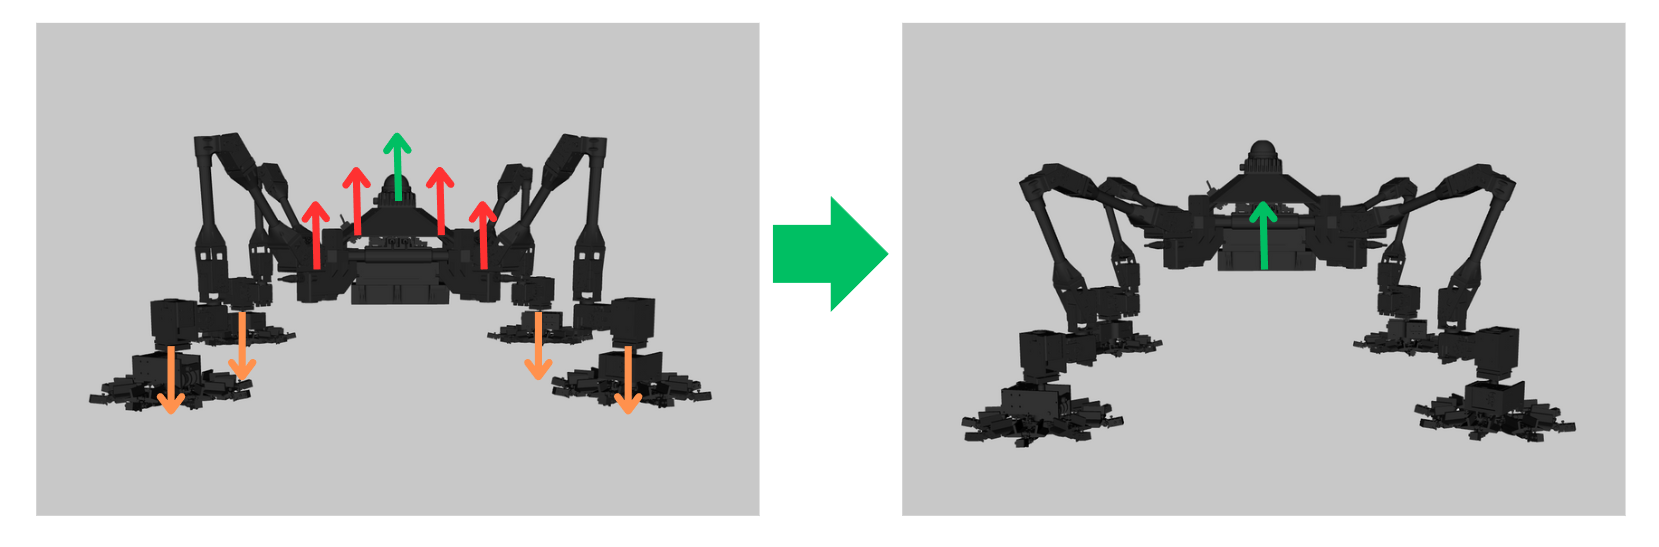
\includegraphics[scale=0.25]{Images/img_ch2/MoveBaseUP.png}
    }
    \quad
    \subfloat[XY translation.\label{fig:MoveBaseBACK}]{
        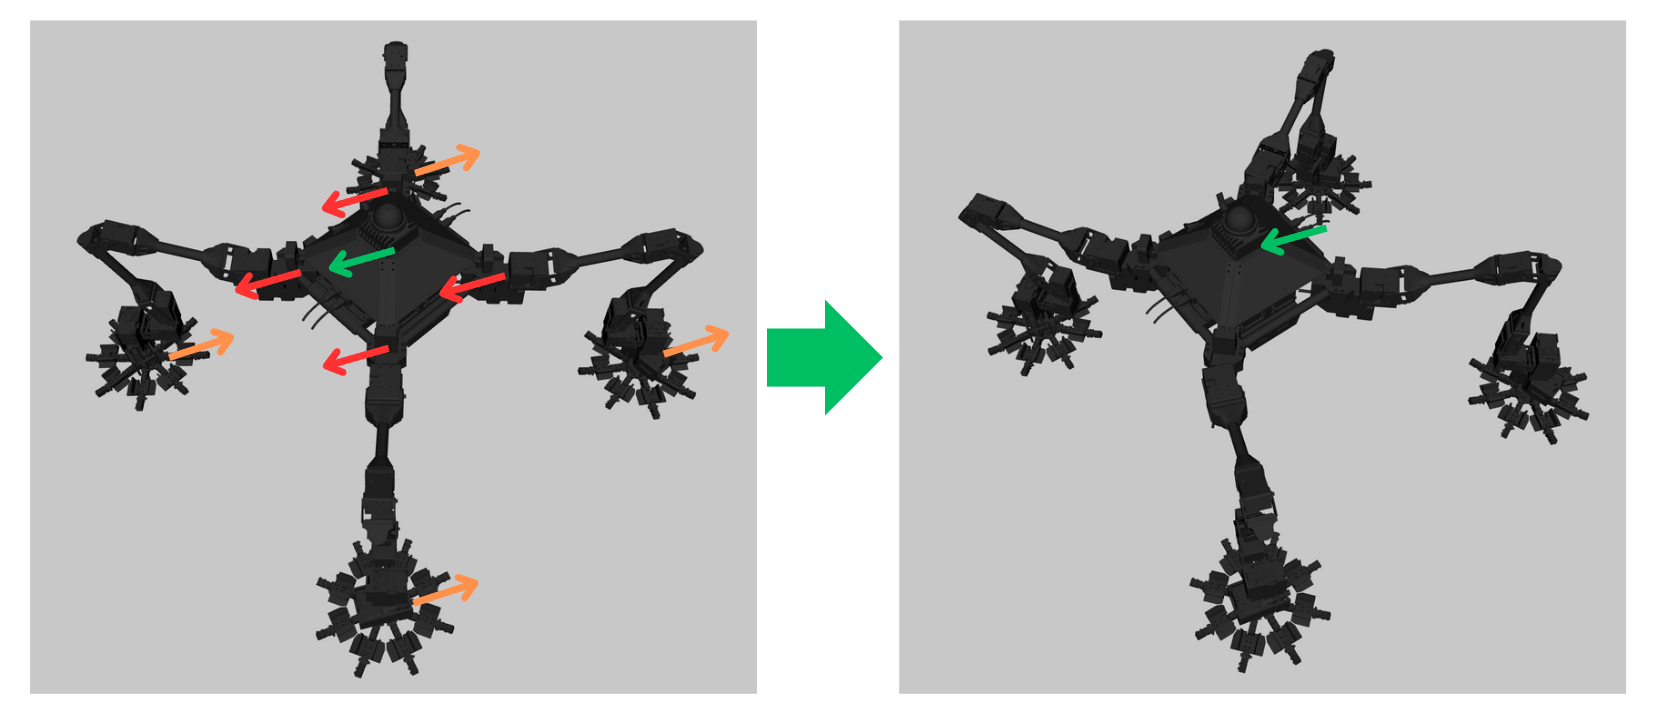
\includegraphics[scale=0.25]{Images/img_ch2/MoveBaseBACK.png}
    }
    \quad
    \subfloat[Yaw rotation.\label{fig:MoveBaseZRotate}]{
        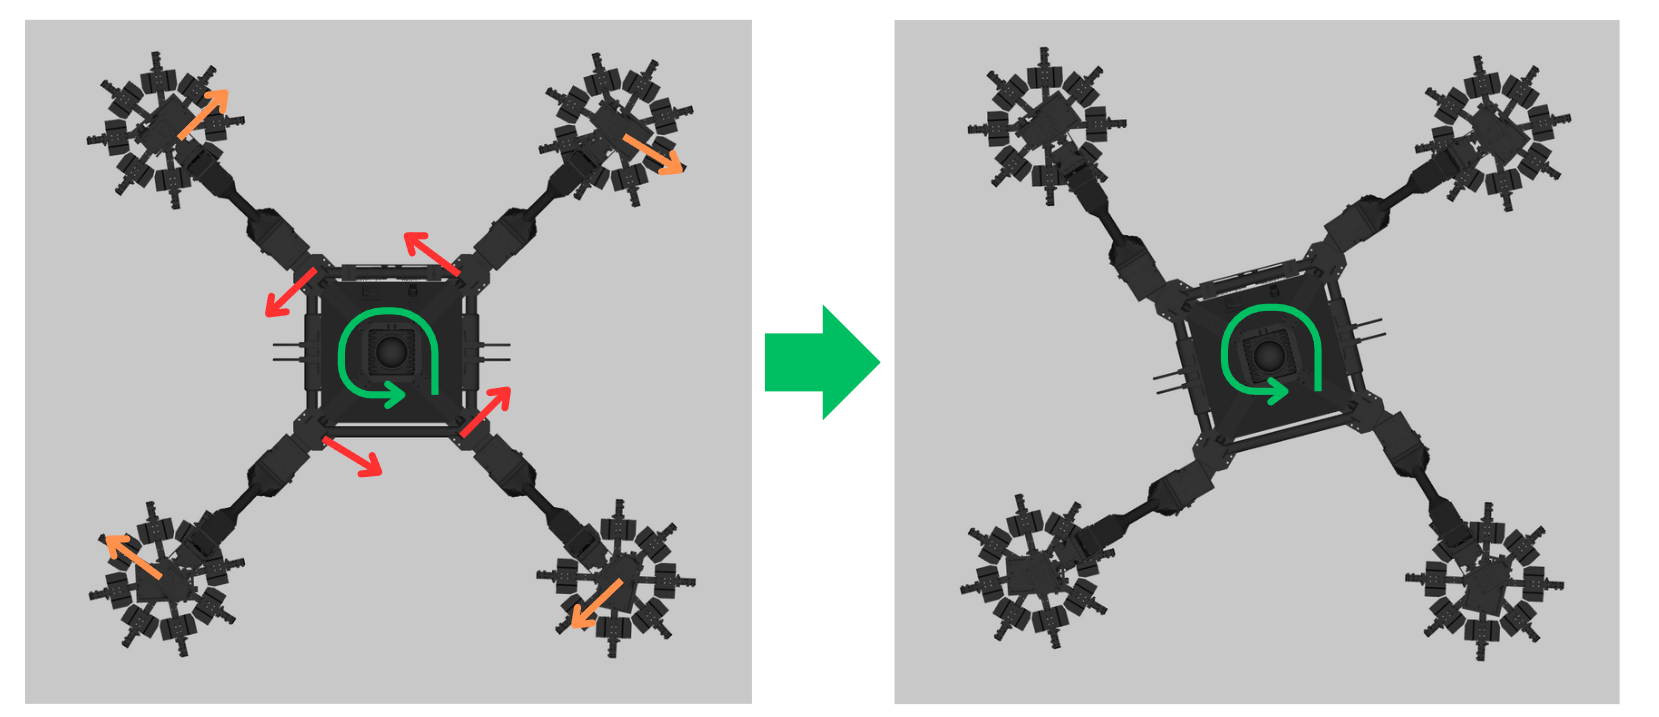
\includegraphics[scale=0.25]{Images/img_ch2/MoveBaseZRotate.png}
    }
    \caption[Limbed Robot IK Motion]{Different base motion as limb motion task. Orange arrows are objective limb position, reds are the new corresponding root pose, and green is the change on the base pose}
    \label{fig:BaseMotionIK}
\end{figure}


\textbf{Parallel Manipulator Model}\newline
Unlike serial manipulators (open chain structures as Fig.\ref{fig:Manipulator}), their parallel counterparts are composed of kinematic
chains with closed subchains (as in Fig.\ref{fig:ParallelManipulator} below).
Two frames can be distinguished, one fixed to the ground,\textit{B}, and one capable of moving arbitrarily within its workspace, \textit{M}.

\begin{figure}[H]
    \centering
    \subfloat[\cite{RoboticMechanics}Parallel manipulator scheme.\label{fig:Parallel}]{
        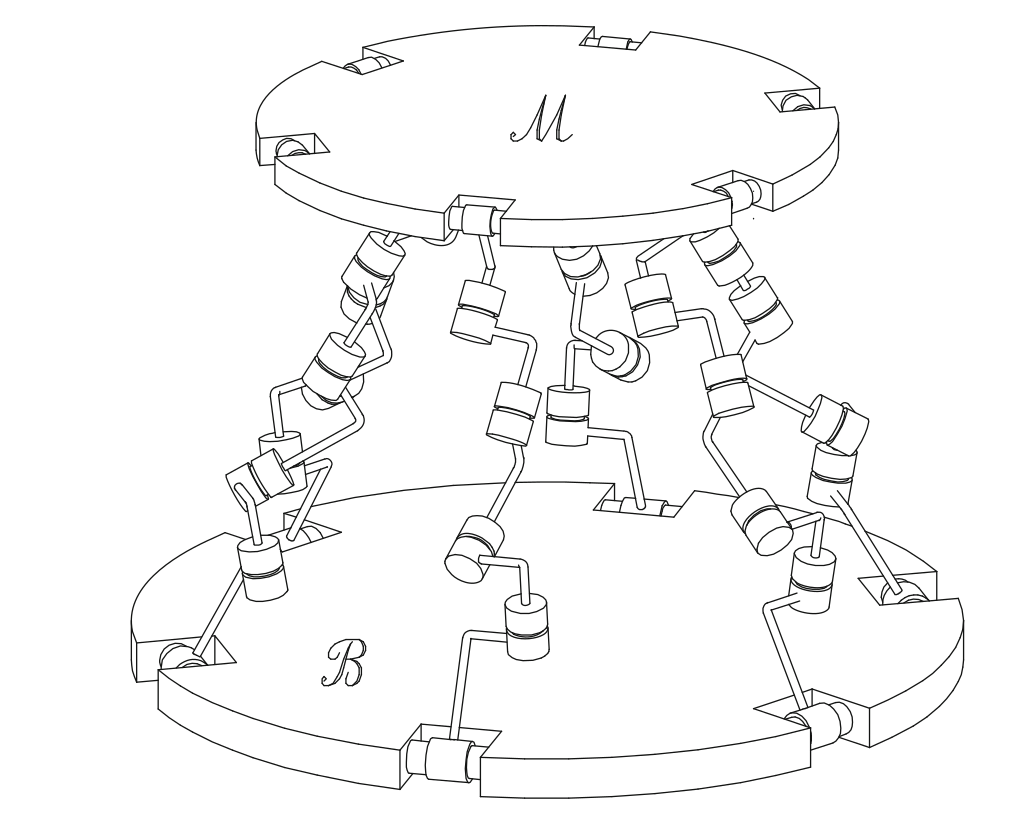
\includegraphics[scale=0.20]{Images/img_ch2/ParallelManipulator.png}
    }
    \subfloat[\cite{ABBParallel}ABB IRB.\label{fig:ABBParallel}]{
        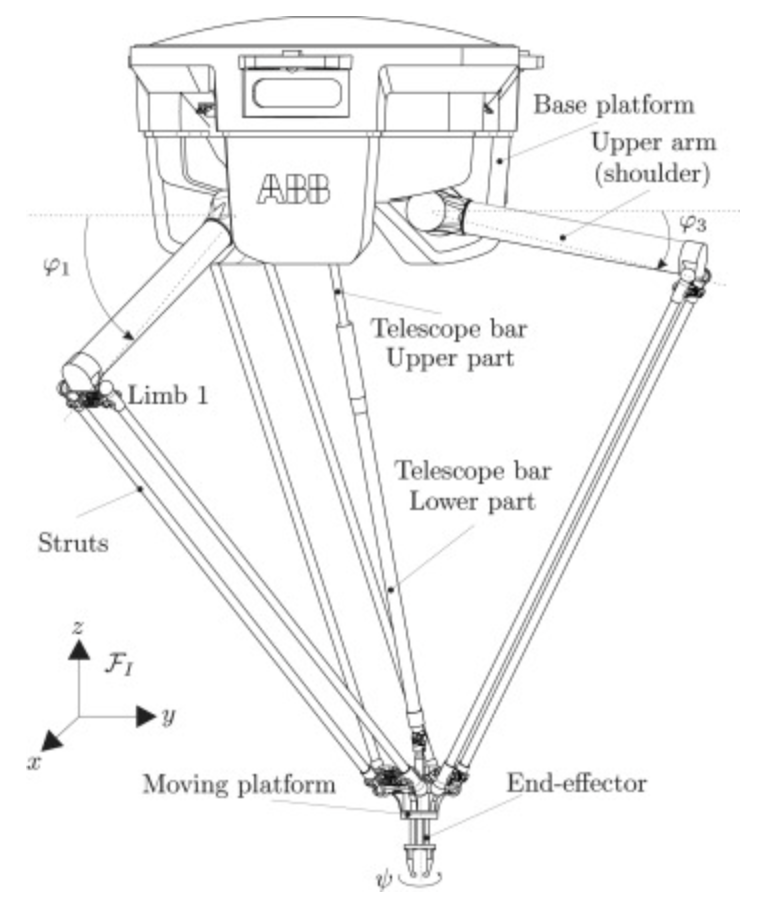
\includegraphics[scale=0.20]{Images/img_ch2/ABB_parallel.png}
    }
    \caption[Parallel Manipulator]{Parallel manipulator general scheme and example}
    \label{fig:ParallelManipulator}
\end{figure}

We can extend the parallel manipulator model\cite{RoboticMechanics} and consider the ground frame \textit{G} as fixed base (previously defined as \textit{B}), and the robot moving base \textit{B} as a moving frame (previously defined as \textit{M}) as in Fig.\ref{fig:KinematicWalkingParallel}.
Each leg is modeled from the contact point to the base root with the classical manipulator model described before. 
 

\begin{figure}[H]
    \centering
    \subfloat[Robot model as parallel manipulator.\label{fig:exapodparallel}]{
        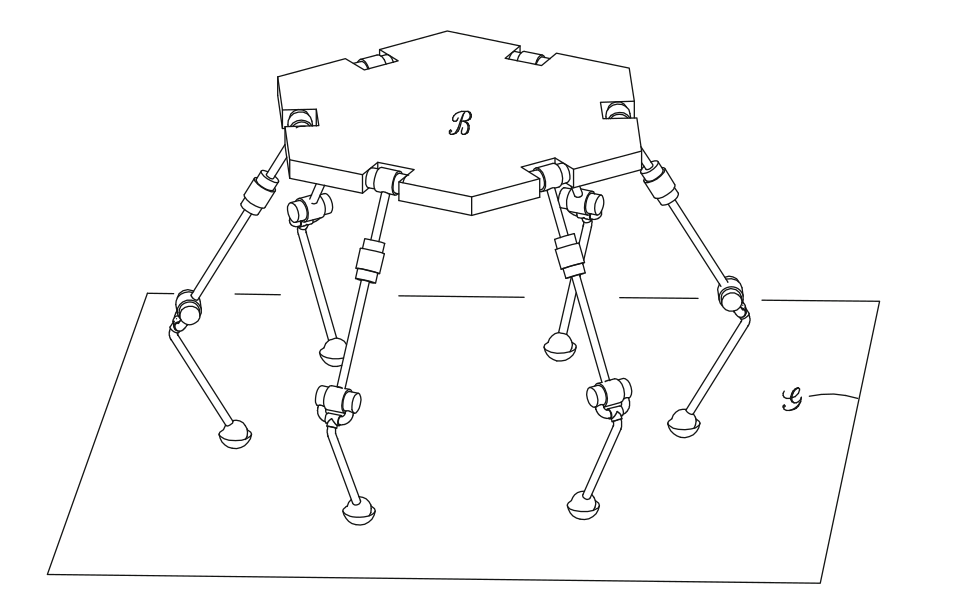
\includegraphics[scale=0.20]{Images/img_ch2/exapod_model.png}
    }
    \subfloat[Limb kinematic model.\label{fig:exapodleg}]{
        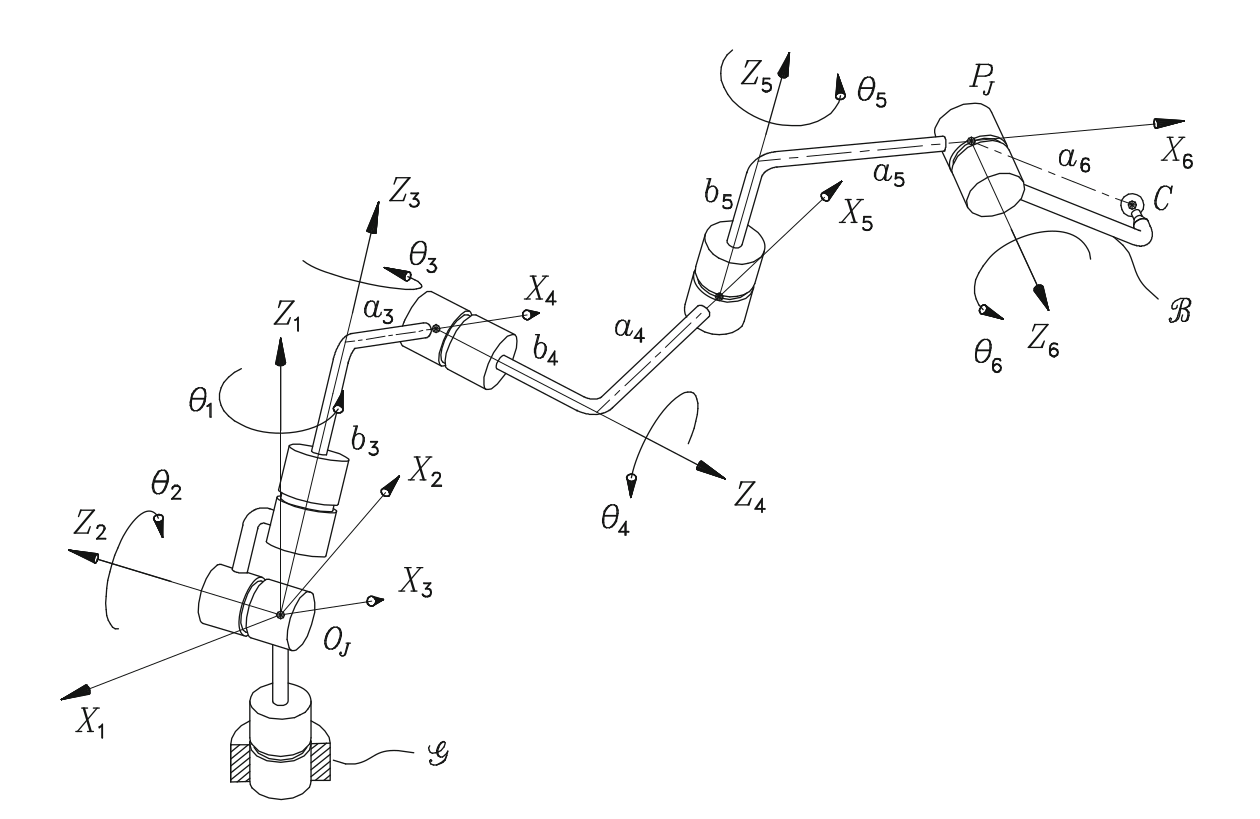
\includegraphics[scale=0.20]{Images/img_ch2/exapod_DH_leg.png}
    }
    \caption[Closed Kinematic chain Leg DH]{\cite{RoboticMechanics} Closed Kinematic chain base motion}
    \label{fig:KinematicWalkingParallel}
\end{figure}


When modeling legged robot base kinematics with the parallelogram structure, legs in contact with the ground are considered. 
Using the same leg kinematic model as in section \ref{sec:leggedFK}, The spherical joint of each leg j $q_{j,1}, q_{j,2},q_{j,3}$ accounts for the coupling of the leg with the ground. This is just for modeling purposes, there is no real actuation on those joints. So, we can reduce the space of actuated joint variables to  $\mathbf
{q_a} \in \mathbb{R}^{n-3N}$, removing all spherical coordinates.
A maneuver of \textit{B}, given by a prescribed pose, can be achieved by
suitable values of the contact limbs actuated-joints $\mathbf
{q_a}$ variables, which thus leads to a problem of parallel-manipulator inverse kinematics\cite{RoboticMechanics}.


\subsection{Differential Kinematic}
\label{sec:differential}
FK and IK have been defined as the direct and inverse mapping between joint space and task space. Such relations capture the robot configuration at a specific time instant. Differential kinematics (DK) instead derives the relationship between joint velocities and final frame linear $\mathbf{\dot{p}_f}$ and angular $\mathbf{\omega_f}$ velocity\cite{Siciliano}.
Denoting the joint space as $\mathbf{\dot{q}} \in \mathbb{R}^n$, and the final frame velocity vector
$\mathbf{v_f} =
\begin{bmatrix}
\mathbf{\dot{p}_f} & \mathbf{\omega_f}
\end{bmatrix}^T$, the mapping is described by: 
\begin{equation}
\label{eq:DK}
    \mathbf{v_f} = \mathbf{J(\mathbf{q})}\cdot\mathbf{\dot{q}} 
\end{equation}

$\mathbf{J(\mathbf{q})}$ is a $6\times n$ matrix, called \textbf{geometrical Jacobian}. This matrix relation can be decomposed into a linear and angular part: 
\begin{equation}
\label{eq:DK_decomposed}
    \mathbf{v_f} =
    \begin{bmatrix}
    \mathbf{\dot{p}_f}\\
    \mathbf{\omega_f}
    \end{bmatrix} = 
    \begin{bmatrix}
    \mathbf{J_P(\mathbf{q})}\\
    \mathbf{J_O(\mathbf{q})}    \end{bmatrix} \cdot \mathbf{\dot{q}} 
\end{equation}

As always, the reference frame is important.
If the notation is expanded, the jacobian matrix relating velocity of frame $\mathbf{f}$ in frame $\mathbf{0}$ can be denoted as $\mathbf{^0J_f}$.
The expression above represents the velocity of the final frame $\mathbf{v_f}$ in a chosen reference frame $\mathbf{0}$ . If velocity has to be represented in frame $\mathbf{k}$, it is easy to do under the hypothesis that $\mathbf{R^k_0}$ is constant \cite{Siciliano}\cite{CorkeMATLAB}. It holds: 

\begin{equation}
\label{eq:VelocityRelation}
    \mathbf{^k v_f} = \begin{bmatrix}
    \mathbf{^k\dot{p}_f}\\
    \mathbf{^k\omega_f}
    \end{bmatrix} =     \begin{bmatrix}
    \mathbf{R^k_0} & \mathbf{0_{3\times 3}}\\
    \mathbf{0_{3\times 3}} & \mathbf{R^k_0} 
    \end{bmatrix} \cdot    \begin{bmatrix}
    \mathbf{^0\dot{p}_f}\\
    \mathbf{^0\omega_f}
    \end{bmatrix} 
\end{equation}

Defining 
$\mathbf{J^k_0} = \begin{bmatrix}
    \mathbf{R^k_0} & \mathbf{0_{3\times 3}}\\
    \mathbf{0_{3\times 3}} & \mathbf{R^k_0} 
    \end{bmatrix}$
, representing a transformation of velocity frames from $\mathbf{0}$ to $\mathbf{k}$, from Eq.\ref{eq:DK}, it is possible to derive the expression of $\mathbf{^k v_f}$:
\begin{equation}
\label{eq:DKFrames}
    \mathbf{^k v_f} = \mathbf{J^k_0} \cdot \mathbf{J(q)} \cdot \mathbf{\dot{q}}
\end{equation}

From now on, the velocity reference frame is neglected, as it depends on the robotic structure under analysis. It will be made explicit only if necessary. 

When the final frame pose is represented in a minimal task space $\mathbf{x_f} \in \mathbb{R}^m$, it is possible to differentiate the forward kinematic relation, obtaining:
\begin{equation}
\label{eq:DK_analytical}
    \mathbf{\dot{x}_f} = \mathbf{J_a(\mathbf{q})}\cdot\mathbf{\dot{q}} 
\end{equation}

The \textbf{analytical Jacobian} $\mathbf{J_a(\mathbf{q})}$ is a $6\times m$ matrix, and in general it is different from the geometric one. 
The Jacobian, not only establishes velocity relation, but the inversion and integration of that relation give us an algorithm to solve IK. 
\begin{equation}
\label{eq:IKfromDK1}
    \mathbf{\dot{q}} = \mathbf{J^{-1}(\mathbf{q})}\cdot    \mathbf{v_f}  
\end{equation}
and then: 
\begin{equation}
\label{eq:IKfromDK2}
    \mathbf{q}(t) = \int_0^t{\mathbf{\dot{q}}(\varsigma)d\varsigma} + \mathbf{q}(0)  
\end{equation}
Obviously, techniques to avoid drifting errors of the integrator are implemented, but it is out of this scope. 

The importance of $ \mathbf{J(\mathbf{q})}$ to be invertible is clear from Eq.\ref{eq:IKfromDK1} . The values of $\mathbf{q}$ for which the Jacobian is not invertible ($det(\mathbf{J(\mathbf{q})}) = 0$, loss of rank) corresponds to a \textbf{singular configuration}. Singularities bring many problems, and so, the analysis of them is crucial for motion planning, and for system design.

The Jacobian matrix is also useful for understanding redundancy, an important concept in robotics, related to the relationship between joint space and task space\cite{Siciliano}\cite{RoboticMechanics}\cite{YoshikawaRedundancy}. A robot is redundant when the dimension of the task space $m$ is less than the joint space $n$, this brings additional freedom, but also complexity. 

Another tool derived from the Jacobian matrix is the \textbf{Manipuilability Ellipsoid} theory, widely expanded and used in this research. This is a geometric representation of the manipulability theory first introduced by T.Yoshikawa\cite{ManipulabilityYoshikawa}, where a hyper-spherical joint-space domain is mapped to a hyper-ellipsoidal task space, in the velocity or force: 
\begin{equation}
\label{eq:EllipsoidVel}
    \mathbf{\dot{q}}^T \mathbf{\dot{q}} = \mathbf{v_f}(\mathbf{J}\mathbf{J}^T)^{-1}\mathbf{v_f} = 1
\end{equation}
\begin{equation}
\label{eq:EllipsoidForce}
    \mathbf{\tau}^T \mathbf{\tau} = \mathbf{\gamma_e}^T(\mathbf{J}\mathbf{J}^T)\mathbf{\gamma_e} = 1
\end{equation}
This concept is expanded in Section \ref{sec:base_manipolability} for this research objective.

Finally, even if not related to kinematics, the Jacobian matrix provides a tool to solve the problem of \textbf{static}:
\textit{The goal of statics is to determine the relationship between the generalized
forces applied to the end-effector and the generalized forces applied to the joints (forces for prismatic joints, torques for revolute joints) with the
manipulator at an equilibrium configuration}\cite{Siciliano}.\\
The \textbf{kinetostatic duality} relationship can be proven with the principle of virtual work, deriving: 

\begin{equation}
\label{eq:Static}
\mathbf{\tau}  = \mathbf{J^T(\mathbf{q})}\cdot\mathbf{\gamma_{e}}
\end{equation}

where $\mathbf{\tau}\in \mathbb{R}^n$ is the vector of joint torques, and  $\mathbf{\gamma_{e}} \in \mathbb{R}^m$ is the vector of final frame generalized forces (force and moments) in task space. 

Again, there are some differences in the analysis of DK for manipulators and legged/limbed robots, which is explored in the next. 

\subsubsection{Manipulators and Single-Leg/Limb}
\label{sec:manipulatorDK}
For serial link structures like a manipulator or a single leg, DK relation is defined as in Eq.\ref{eq:DK}, with the same notation used for FK.
Fig.\ref{fig:ArmLegDK} represents an intuitive view of DK relation. 
If the frames are assigned using the DH convention, $\mathbf{J(\mathbf{q})}$ is derived column by column as: 
\begin{equation}
\label{eq:JacobianFormulaArm}
    \begin{bmatrix}
    \mathbf{j_{Pi}(\mathbf{q})}\\
    \mathbf{j_{Oi}(\mathbf{q})}    \end{bmatrix} = 
    \begin{cases}
    \begin{bmatrix}
    \mathbf{z_{i-1}}\\
    \mathbf{0}  \end{bmatrix}  \text{ if $i$ is prismatic}\\ \\ 
    \begin{bmatrix}
    \mathbf{z_{i-1}} (\mathbf{p_{e}} -  (\mathbf{p_{i-1}})\\
    \mathbf{z_{i-1}}\end{bmatrix} \text{ if $i$ is revolute}
    \end{cases}
\end{equation}

If the frames are not assigned with the DH convention, it is still possible to derive $\mathbf{J(\mathbf{q})}$ without this standard formulation.  
Furthermore, in terms of reference frame, Eq.\ref{eq:JacobianFormulaArm} provide the expression of $\mathbf{^b J_e(q)}$ (velocity of end-effector in base frame) or $\mathbf{^r J_f(q)}$ (velocity of foot/leg-tip in root frame), Eq.\ref{eq:DKFrames} is used for a change of reference frame (for example, to move to world \textbf{w} frame or legged/limbed body frame \textbf{b}).

The vectors in the statics equation \ref{eq:Static} in this case are: all the arm or leg/limb joint torques $\mathbf{\tau} \in \mathbb{R}^n$ and the generalized force applied at the end-effector or leg/limb-tip $\mathbf{\gamma_{e/f}} \in \mathbb{R}^m$.
For example, in 3D space it can be $m= 6$ and  $\mathbf{\gamma_{e/f}} = \begin{bmatrix}
    f_x & f_y & f_z & \mu_x & \mu_y & \mu_z
\end{bmatrix}^T$

\begin{figure}[H]
    \subfloat[DK of robotic arm.\label{fig:ArmDK}]{
    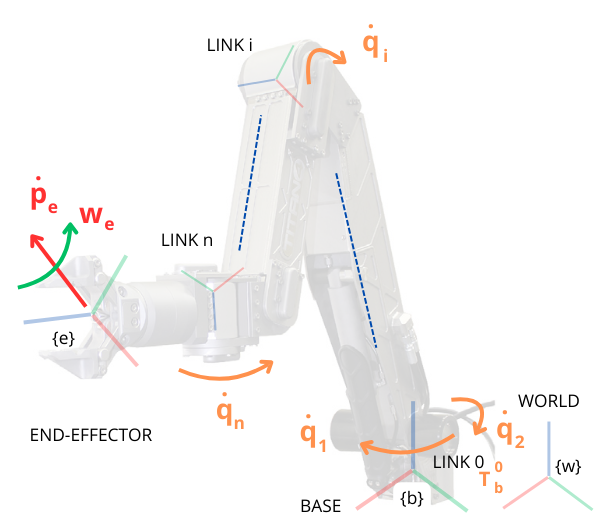
\includegraphics[scale=0.45]{Images/img_ch2/ArmDK.png}
    }
    \subfloat[DK of root-foot robotic leg/limb.\label{fig:LegDK}]{
        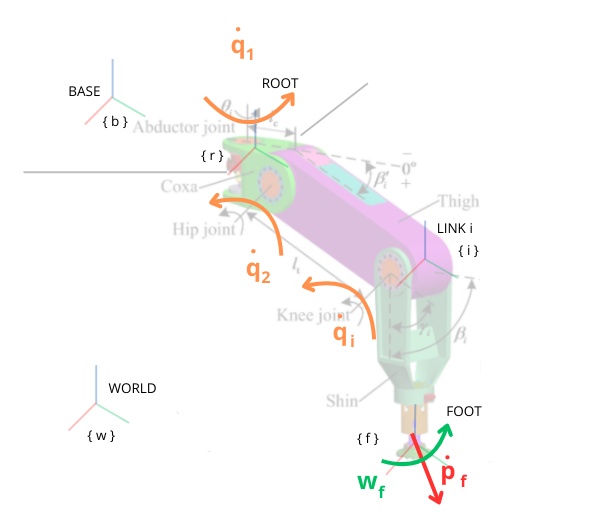
\includegraphics[scale=0.50]{Images/img_ch2/LegDK.png}
    }
    \caption[Arm and Leg/Limb DK]{Arm and Leg/Limb DK}
    \label{fig:ArmLegDK}
\end{figure}

\subsubsection{Legged/Limbed Robots Base}
\label{sec:leggedLimbedDK}
As discussed in the previous sections about FK and IK, the kinematics of N-legged/limbed robots involves the analysis of the base motion.
With reference to Fig.\ref{fig:LeggedDK},
the final goal is to derive a $6 \times n, (n=\sum_{j=1}^Nn_j)$ Jacobian matrix $\mathbf{J(q)}$ representing the relationship between
all legs/limbs joints velocity $\mathbf{\dot{q}} \in \mathbb{R}^n$ and the base velocity $\mathbf{v_b} = \begin{bmatrix}
\mathbf{\dot{p}_b} & \mathbf{\omega_{b}}\end{bmatrix}^T $ .

\begin{figure}[H]
    \centering
    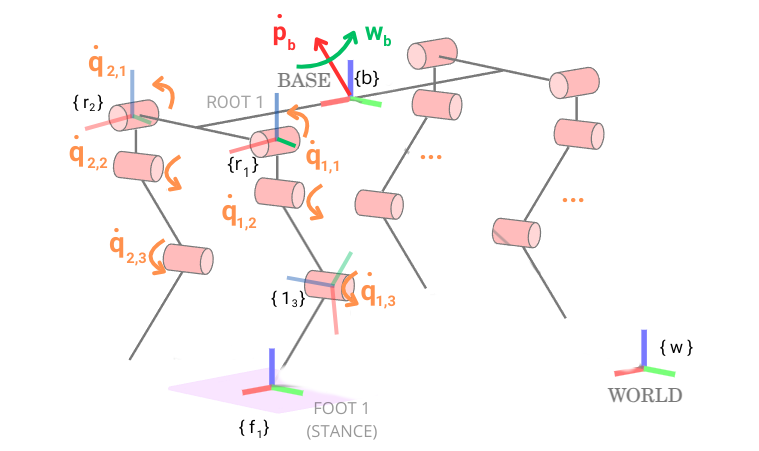
\includegraphics[width=0.9\textwidth]{Images/img_ch2/LeggedDK.png}
    \caption{Legged robot DK relation}
    \label{fig:LeggedDK}
\end{figure}

An alternative way to define the base velocity is $\mathbf{\dot{q}_b}$ through the \textbf{floating base model}, described previously. 

Different methods exist to derive this relationship, according to the kinematic model used. 
If the \textbf{parallel manipulator model} is used to describe the robot, theory on differential kinematics for closed chain structures exists \cite{Siciliano}\cite{RoboticMechanics}.
To define the contact point-to-root kinematic model, one of the two approaches expressed previously is possible: 
\begin{enumerate}
    \item Extend the leg/limb model with a spherical joint and model the system inverting joint order (used for the parallel manipulator model).
    \item use the contact leg/limb motion propagation without penetration approach, as defined in section\ref{sec:leggedLimbedIK}. 
\end{enumerate}

method (2) is employed in this thesis.
From now on, the Jacobian matrix and velocity vectors' reference frame is important, so it is explicit.
From the relation $\mathbf{^{e_j}v_{r_j}} = -\mathbf{^{r_j}v_{e_j/f_j}}$, it is just a matter of solving DK for the open chain root-to-tip leg/limb model (as in Eq.\ref{eq:DK}): 
\begin{equation*}
\label{eq:LegDKInversed1}
 \mathbf{^{r_j}v_{{e_j}/{f_j}}} = \mathbf{{^{r_j}J_j}(q_j)}\cdot\mathbf{\dot{q}_j}
\end{equation*}
so, with the velocity relation assumed before:
\begin{equation}
\label{eq:LegDKInversed2}
 \mathbf{^{e_j/f_j}v_{r_j}} = -\mathbf{{^{r_j}J_j}(q_j)}\cdot\mathbf{\dot{q}_j}
\end{equation}

The velocity vector $\mathbf{^{e_j/f_j}v_{r_j}}$ is equivalent to the velocity of one of the cooperative manipulators' end-effector (corresponding to the limb root), measured in its base frame (the contact foot/limb-tip). This parallelism is represented in Fig.\ref{fig:MultiArmLimbed}  

If we want to compute velocity of the limb root $\mathbf{^b v_{r_j}}$, measured on the base frame: 
\begin{equation}
\label{eq:rootDK_baseframe}
 \mathbf{^b v_{r_j}} = -\mathbf{J^b_{r_j}}\mathbf{{^{r_j}J_j}(q_j)}\cdot\mathbf{\dot{q}_j} = \mathbf{^b J_j(q_j)}\cdot\mathbf{\dot{q}_j}
\end{equation}

The ideas of \textbf{cooperative manipulators}\cite{CooperativeManipulators}\cite{DualArmManipulability}\cite{MultiArmManipulability} give a different point of view. Each leg/limb in contact with the ground $j \in J_c$ can be modeled from the contact point to the root as a separate "manipulator", cooperating to move the base frame. This is a novel approach for legged/limbed robots, introduced in this research, the details on this theory are addressed in in section \ref{sec:base_manipolability} of the next chapter.


\begin{figure}[H]
    \centering
    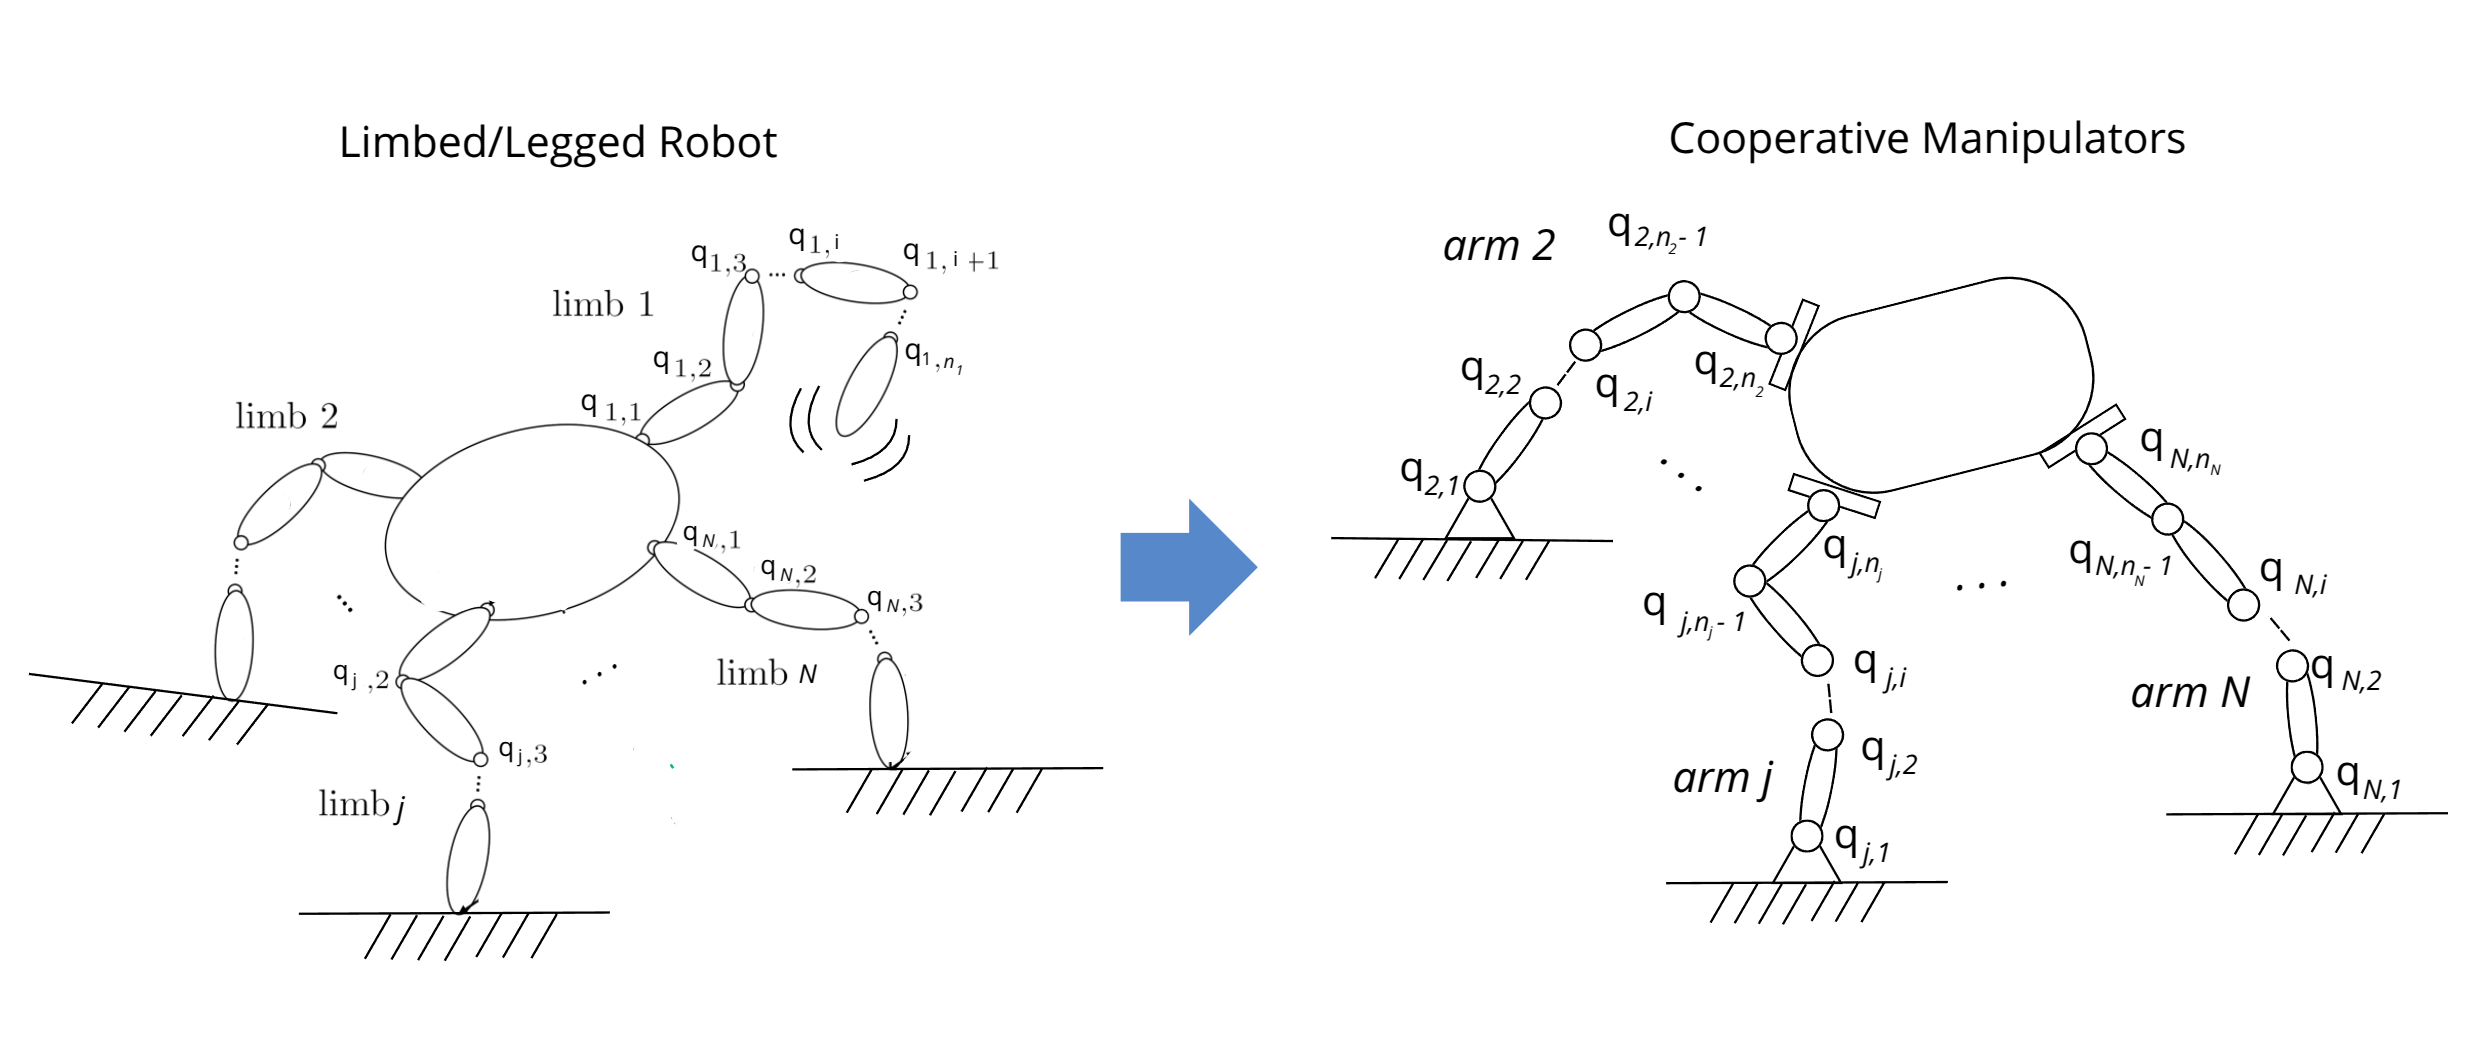
\includegraphics[width=1.0\textwidth]{Images/img_ch2/MultiArmLimbedParallel.png}
    \caption{Parallelism between limbed/legged robot and cooperative manipulator}
    \label{fig:MultiArmLimbed}
\end{figure}

The final relationship derived from this approach is again in the form: 
\begin{equation}
\label{eq:LeggedMultiArm}
 \mathbf{v_b} = \mathbf{{J}(q)}\cdot\mathbf{\dot{q}}
\end{equation}

\section{Dynamic Model}
\label{sec:dynamic}
Dynamics complete the modeling tools needed to analyze and understand the motion of a mechanical system. While kinematics forget about the cause of motion, 
the objective of \textbf{dynamics modeling} is to derive the relationship between joint actuator torques and the motion of the structure\cite{Siciliano}. 
The dynamics model is fundamental to derive the systems' equations of motion (EoM), then used for \textbf{simulation} and \textbf{design of control algorithms}.

To derive those equations, two methods exist: 
\begin{itemize}
    \item \textbf{Lagrange formulation}: Systematic approach, based on energetic quantities differentiation. 
    Defining the Lagrangian function as $\mathcal{L} = \mathcal{T} - \mathcal{U}$ (where $\mathcal{T}$ and $\mathcal{U}$ are respectively the kinematic and potential energy of the mechanical system) and $\mathbf{\xi}$  the vector of generalized force associated to the joint variables $\mathbf{q}$:
    \begin{equation}
    \label{eq:Lagrangian}
     \frac{d}{dt}\left(\frac{\partial\mathcal{L}}{\partial\mathbf{\dot{q}}}\right)^T -  \left(\frac{\partial\mathbf{\mathcal{L}}}{\partial\mathbf{q}}\right)^T= \mathbf{\xi}
    \end{equation}

    \item \textbf{Newton-Euler formulation}: based on a balance of forces and moments for rigid bodies.
    Recursive algorithms to solve dynamics are often based on this approach\cite{Siciliano}. 
\end{itemize}

The Lagrange formulation is the method employed here because it derives the EoM in a compact analytical form, convenient for control design.  
Furthermore, dynamics branches into two problems: 
\begin{itemize}
    \item \textbf{Direct Dynamics}:\\
    \textit{Given initial joint state and velocity $\mathbf{q}(t_0)$, $\mathbf{\dot{q}}(t_0)$, applied external generalized forces at final frame $\mathbf{h_e}(t)$ and joint torques $\mathbf{\tau}(t)$ for $t>t_0$, determine joint acceleration $\mathbf{\ddot{q}}(t)$ for $t>t_0$.}\\
    Once this problem is solved, from $\mathbf{\ddot{q}}(t)$, it is possible to integrate and obtain $\mathbf{\dot{q}}(t)$, $\mathbf{q}(t)$, and then from kinematics, describe the motion of the frame of interest. This is the procedure used to simulate motion.  
    \item \textbf{Inverse Dynamics}: \\
    \textit{Given the desired joint motion $\mathbf{\ddot{q}}(t)$, $\mathbf{\dot{q}}(t)$, $\mathbf{q}(t)$ and knowing the external external generalized forces at final frame  $\mathbf{h_e}(t)$, determine the joint torques $\mathbf{\tau}(t)$ to achieve that motion.}\\
    Algorithms to control the system can be derived from the solution to this problem\cite{SurveyQuadrupeds}.    
\end{itemize}

Next, a brief survey of the EoM derived from the dynamics of some robotic structures is presented.

\subsection{Manipulators and Single-Leg/Limb}
\label{sec:manipulatorDyn}
The theory on Manipulator robots is well-established, and a standard EoM in matrix form is derived with the Lagrange approach: 
\begin{equation}
    \label{eq:ManipulatorEoM}
    \mathbf{B}(\mathbf{q})\mathbf{\ddot{q}} + \mathbf{C}(\mathbf{q},\mathbf{\dot{q}})\mathbf{\dot{q}} + \mathbf{F_v\dot{q}} + \mathbf{F_{s}}sgn(\mathbf{\dot{q}})+ \mathbf{g}(\mathbf{q}) = \mathbf{\tau} - \mathbf{J}^T(\mathbf{q})\mathbf{h_e}
\end{equation}
Where the matrices have the following meaning: 
\begin{table}[H]
    \begin{tabular}{ll}
        ${\mathbf{B}(\mathbf{q})}$ & Inertia Matrix ($n \times n$, symmetric and positive definite).\\[2pt]
        ${\mathbf{C}(\mathbf{q}, \mathbf{\dot{q}})}$ & Coriolis and Centrifugal Matrix ($n \times n$).\\[2pt]
        $\mathbf{F_v}$ & Viscous friction matrix ($n \times n$, diagonal).\\[2pt]
        $\mathbf{F_s}$ & Static friction matrix ($n \times n$, diagonal), coulomb friction model.\\[2pt]
        $\mathbf{g}(\mathbf{q})$ & Gravitational torque vector ($n \times 1$).\\[2pt]
   \end{tabular}
\end{table}
The other symbols have the same meaning as discussed before. 
In particular, $\mathbf{J}^T(\mathbf{q})\mathbf{h_e}$ map the generalized force exerted by the EE to the joint space (similarly to the static relationship \ref{eq:Static}). When a generalized force $\mathbf{h_c}$ is applied at a generic point $\mathbf{C}$ in the structure, the mapping is straightforward, an additional contribution of $\mathbf{\tau_c} = \mathbf{J_c}^T(\mathbf{q})\mathbf{h_c}$ is subtracted at the left-hand side of the EoM \cite{DeLucaContact1}. 

The dynamic model above is highly coupled and configuration-dependent, for control purposes, a decoupled joint model can be derived. 

\subsubsection{Decoupled Model}
\label{sec:DecoupledDyn}
The joint space vector $\mathbf{q}$ used until now, refers to the change of position of the link from the initial one, neglecting what happens at the motor level. 
Gearboxes are usually used for joint actuation, a gearbox provides a mechanical transmission between the motor and load, with reference to Fig.\ref{fig:TransmissionMotor}, the following relationship holds: 
\begin{equation}
\label{eq:Transmission}
    \begin{cases}
        q_l = \frac{1}{N_{gear}}q_m \\
        \dot{q}_l = \frac{1}{N_{gear}}\dot{q}_m \\
        \mathbf{\tau}_{l} = N_{gear} \mathbf{\tau}_{lm} \\
    \end{cases}
\end{equation}
Where $N_{gear}$ is the transmission ratio (or gear ratio), $\tau_l$ the torque at the load side (corresponding to $\tau_i$, $i^{th}$ joint torque of $\mathbf{\tau}$),  $\tau_{lm}$ the load torque transferred at motor side, $\tau_{m}$ the motor torque, $J_m$ the motor inertia, and $J_l$ the load inertia.
Neglecting the friction effect, the motor dynamics is defined by the following equation: 
\begin{equation}
\label{eq:Transmission}
        J_{m}\ddot{q}_m = \tau_m - \frac{\tau_l}{N_{gear}} 
\end{equation}

\begin{figure}[H]
    \centering
    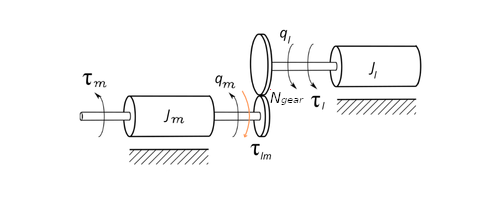
\includegraphics[width=1.0\textwidth]{Images/img_ch2/TransmissionMotor.png}
    \caption{\cite{Siciliano} Schematic representation of mechanical gear }
    \label{fig:TransmissionMotor}
\end{figure}

Considering a single row of the dynamic equation of the manipulator (neglecting external forces and friction), the load torque for the $i^{th}$ motor-transmission-load system is:
\begin{equation*}
    \label{eq:ManipulatorJointEoM}
    \tau_i = \mathbf{B_i}^T(\mathbf{q})\mathbf{\ddot{q}} + \frac{1}{2}\mathbf{\dot{q}}^T\mathbf{C_i}(\mathbf{q})\mathbf{\dot{q}} + g_i(\mathbf{q}) 
\end{equation*}
Then, collecting as residual the effect of Coriolis and centrifugal forces, gravitational load, and other joints ($j \not{=} i$) inertial effect: 
\begin{equation*}
    \label{eq:ResidualManipulator}
    \tau_{di} = \sum_{j\not{=}i}{C_{ij}(\mathbf{q})\cdot\dot{q}^2_j} +\sum_{j\not{=}i}{B_{ij}(\mathbf{q})\cdot\ddot{q}_j} + g_i(\mathbf{q})
\end{equation*}
And approximating $B_{ii}(\mathbf{q})$, representing the effect of inertia of joint $i$ due to its acceleration, as $B_{ii}(\mathbf{q}) \simeq \overline{B_{ii}} = J_{li}$ (as an average value over frequent joint configurations), the equation for $i^{th}$ joint become: 
\begin{equation*}
    \label{eq:TauJoint}
    \tau_i = J_{li}\ddot{q}_i + \tau_{di}
\end{equation*}
Introducing this load torque in Eq.\ref{eq:Transmission}, the resulting decoupled model, represented in Fig.\ref{fig:ManipulatorDecoupled} is: 
\begin{equation}
    \label{eq:DecoupledManipulatorEoM}
    \left ( J_{mi} + \frac{J_{li}}{N_{gear,i}^2}\right )\ddot{q}_{mi} = \tau_{mi} - \frac{\tau_{di}}{N_{gear,i}} \quad i = 1,\dots,n
\end{equation}

It is important to notice that the residual term $\tau_{di}$ is scaled up by $N_{gear,i}$, meaning that, high reduction ratios reduce the coupling effects, making the independent joint model a more accurate approximation. 
\begin{figure}[H]
    \centering
    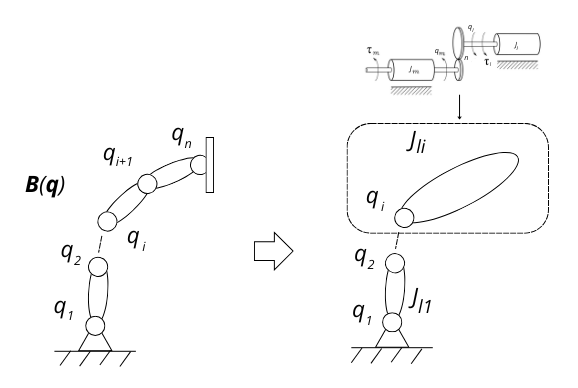
\includegraphics[width=0.75\textwidth]{Images/img_ch2/IJC.png}
    \caption{Schematic representation of decoupled manipulator model}
    \label{fig:ManipulatorDecoupled}
\end{figure}


Under the assumption that the base of a legged/limbed robot is static, the same equations describe a single leg/limb model from the root to the tip. 
In particular, this is useful in multipurpose multi-limb robots, when manipulation tasks are assigned, the EoM of the single limb can be considered as in Eq.\ref{eq:ManipulatorEoM} or Eq.\ref{eq:DecoupledManipulatorEoM}.

\subsection{Legged Robots, Walking Machines}
\label{sec:leggedDyn}

The mechanical complexity of walking robots and their intrinsic closed kinematic chain has been commented on several times. For this reason, forces and moments propagate from one leg to another, further increasing coupling effects. 
Considering the different approaches for walking robots discussed before, if a "stance-foot" modeling approach is used, the parallel manipulator model can be used, where only contact legs are considered. The dynamic model of parallel manipulator \cite{RoboticMechanics} with a minimal DOF as all leg joints can be derived. With this modeling approach, changing the stance foot causes a switch in the dynamic model, making the dynamics model a state machine with a number of states exponential in the number of legs.  
If instead a non-minimal number of DOF is used and the floating base DOFs model is employed, ( previously defined as: $\mathbf{q} = \begin{bmatrix}
    \mathbf{q_b} & \mathbf{q_1} & \mathbf{q_2} & \dots & \mathbf{q_N}
\end{bmatrix}^T$) it is possible to derive the EoM in a standard form with the Lagrange approach\cite{QuadrupedLocomotion}\cite{HandbookLegged} $\mathbf{q} \in \mathbb{R}^{n+6}, (n=\sum_jn_j)$: 
\begin{subequations}
    \label{eq:WalkingDyn}
    \begin{align}[left=\empheqlbrace]
           \mathbf{B}(\mathbf{q})\mathbf{\ddot{q}} + \mathbf{C}(\mathbf{q},\mathbf{\dot{q}})\mathbf{\dot{q}}+ \mathbf{g}(\mathbf{q}) = \mathbf{J_M}^T(\mathbf{q})\mathbf{\tau} - \mathbf{J_C}^T(\mathbf{q})\mathbf{h_c} \label{eq:WalkingEoM} \\
    \mathbf{J_c}\ddot{\mathbf{q}} + \mathbf{\dot{J}_c}\dot{\mathbf{q}} = 0\label{eq:walkingEoMConstraint} 
    \end{align}
\end{subequations}

Eq.\ref{eq:walkingEoMConstraint} represents the holonomic contact constraint of null velocity at contact point $\mathbf{v_c} = \mathbf{J_c}(\mathbf{q})\mathbf{\dot{q}} = \mathbf{0}$, and 
the matrices involved include the self and coupling effects of all leg joints and base DOF, so they have bigger dimensions than Eq.\ref{eq:ManipulatorEoM}. The matrix $\mathbf{J_M}$ maps all leg joint torques in the space of generalized coordinates.

Under some assumptions, the dynamics can be simplified\cite{Legged}\cite{HumanoidRobot}\cite{HandbookLegged}\cite{ModelingControlLegged}, providing a tool for the dynamical analysis of the robot, simple simulation, and controller design.  

For example, as described in \cite{ModelingControlLegged}\cite{Legged}\cite{ArticulatedRobots}, the non-actuated (virtual DOF of the base) part of the EoM can be rewritten as the Newton-Euler equation of the whole system: 
\begin{equation}
    \label{eq:CoMDynamicWalking}
    m(\ddot{\mathbf{c}} + \mathbf{g}) = \sum_i{f_i}
\end{equation}

Where $\mathbf{c}$ is the position of the whole robot CoM, $\mathbf{g}$ is the vector of gravity, and $f_i$ are the external forces. 
Equation \ref{eq:CoMDynamicWalking} doesn't provide details on the controlled DOFs, but it is important because it highlights that to generate any motion ($\ddot{c} \not= 0$) different from the gravitational falling effect, interaction forces $f_i$ are needed, so the goal of any motion algorithms will be to achieve a proper ground interaction.
Other models include the cart-table and the inverted pendulum\cite{Todd}.


\subsection{Limbed Robots, Multipurpose Machines}
\label{sec:limbedDyn}
If modeling the dynamics of walking robots is complex, for multi-limbed multipurpose robots it is even harder. The main difference is in the interaction of each limb with the environment. In Eq.\ref{eq:WalkingEoM}, the external force $\mathbf{h_c}$ model ground interaction during walking locomotion, only as pushing force, usually modeled using contact model as the friction cone \cite{ModelingControlLegged}\cite{WBCFocchi}. For multi-limb robots instead, the interaction can include manipulation and so additional payload, climbing with pushing forces\cite{RibeiroGroundGripping}, and hybrid wheeled-legged locomotion\cite{AnymalDocThesis}. An equation similar to \ref{eq:WalkingEoM} can be derived, but the modeling of $\mathbf{h_c}$ becomes harder. 

\section{Motion Control, State of the Art}
\label{sec:motionControl}

The objective of motion control is to enable the system's autonomy, and two main approach are used in controlling robotics systems\cite{LeggedSurvey}\cite{InteligentControlMultiLegged}: 
\begin{itemize}
    \item \textbf{Model Based}: the control algorithm exploits the knowledge of kinematics or dynamics model to compute the control action.
    \item \textbf{Model Free}: novel emerging approach like Reinforcement Learning\cite{AnymalDocThesis}\cite{RL_overview}, where the system learns a policy to execute tasks in the best way. 
\end{itemize}

In robotics, model-based algorithms are intrinsically multi-layered, the problem can be generalized in the following steps: 
\begin{enumerate}
    \setlength\itemsep{-0.7em} 
    \item Definition of the task (high-level)
    \item Conversion of task into system DOFs (middle-level)
    \item Actuation of DOFs (low-level)
\end{enumerate}

Each level has more functions, and
the accuracy and reliability of control can be ensured only when the system state is continuously observed, implementing a \textbf{feedback} control strategy\cite{Siciliano}\cite{CorkeMATLAB}. 

This closed-loop control principle is defined as the "sense-plan-act" architecture (in Fig.\ref{fig:RobotControl}), composed of the main components to achieve autonomy:
\begin{itemize}
    \setlength\itemsep{-0.7em} 
    \item \textbf{sensors}: To perceive the internal state (proprioceptive) and the surroundings (exteroceptive)
    \item \textbf{actuators}: To effectively interact with the environment and perform actions.
    \item \textbf{controllers}: connect perception and action by a control logic, as the one defined above.  
\end{itemize}

\begin{figure}[H]
    \centering
    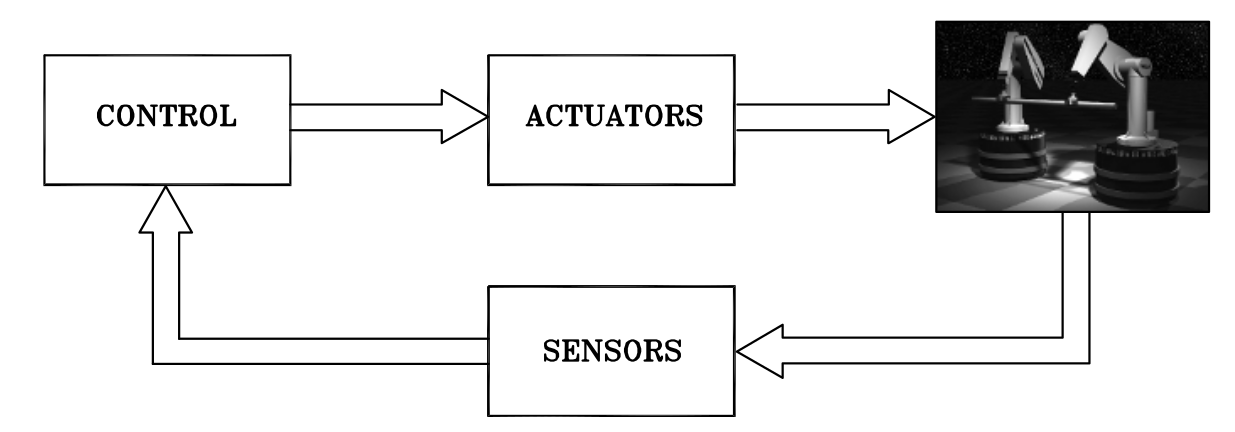
\includegraphics[width=0.7\textwidth]{Images/img_ch2/RobotControl.png}
    \caption{\cite{Siciliano} Closed loop sense-plan-act architecture}
    \label{fig:RobotControl}
\end{figure}

Next, the control architecture for manipulators is defined, then, legged and multi-limbed robots are discussed.  

\subsection{Manipulators}
\label{sec:manipulatorControl}

In manipulator robots, the desired task is defined by a sequence of the EE positions, to be reached autonomously without colliding with obstacles. The main functions of the control architecture layer, represented in Fig.\ref{fig:ManipulatorControlScheme}, are: 
\begin{itemize}
    \setlength\itemsep{-0.7em} 
    \item \textbf{High-Level}: Tasks are generated autonomously by intelligent decision algorithms or by an operator.
    \item \textbf{Middle-Level}:  After generating the trajectory between the initial state (computed with FK from joint feedback) and the final state in EE coordinates, tasks are converted in joint space by IK. Then a control algorithm is used to compute the actuator input from the joint state reference.  
    \item \textbf{Low-Level}: Closed loop control of actuator command, like the motor torque's proportional integral derivative (PID) feedback control. 
\end{itemize}

Additionally, \textbf{state estimator} algorithms are included to keep track of the internal state of the system from sensor feedback.

The high-level task generator can be operated manually, or with more intelligent algorithms ensuring a complete level of autonomy. 
For example, in pick and place tasks or in machining, feedback from cameras and other sensors is used to generate the sequence of operations once the general task has been defined\cite{CorkeMATLAB}. 

For the middle-level control layer, only the control in the joint space is described here, but working directly in the task space is possible with appropriate algorithms\cite{Siciliano}. 

There are different choices for the control algorithms in the \textbf{axis controller}, which is responsible for moving the joints in the desired position, in the \textbf{model based} context,  some of the most common are: 
\begin{itemize}
    \setlength\itemsep{-0.7em} 
    \item \textbf{Indipendent Joint Control} (IJC): Decentralized control, based on the decoupled model defined in Eq.\ref{eq:DecoupledManipulatorEoM}.
    \item \textbf{Inverse Dynamics} (ID): From the desired joint state, dynamics equation \ref{eq:ManipulatorEoM} is solved in $\mathbf{\tau}$. This approach requires an accurate estimation of dynamic model parameters, often hard to obtain. 
    \item \textbf{Adaptive}: Based on adaptive control theory. 
    \item \textbf{Model Predictive Control} (MPC): Find the best control input as an optimization problem using the system model. 
\end{itemize}

\begin{figure}[H]
    \centering
    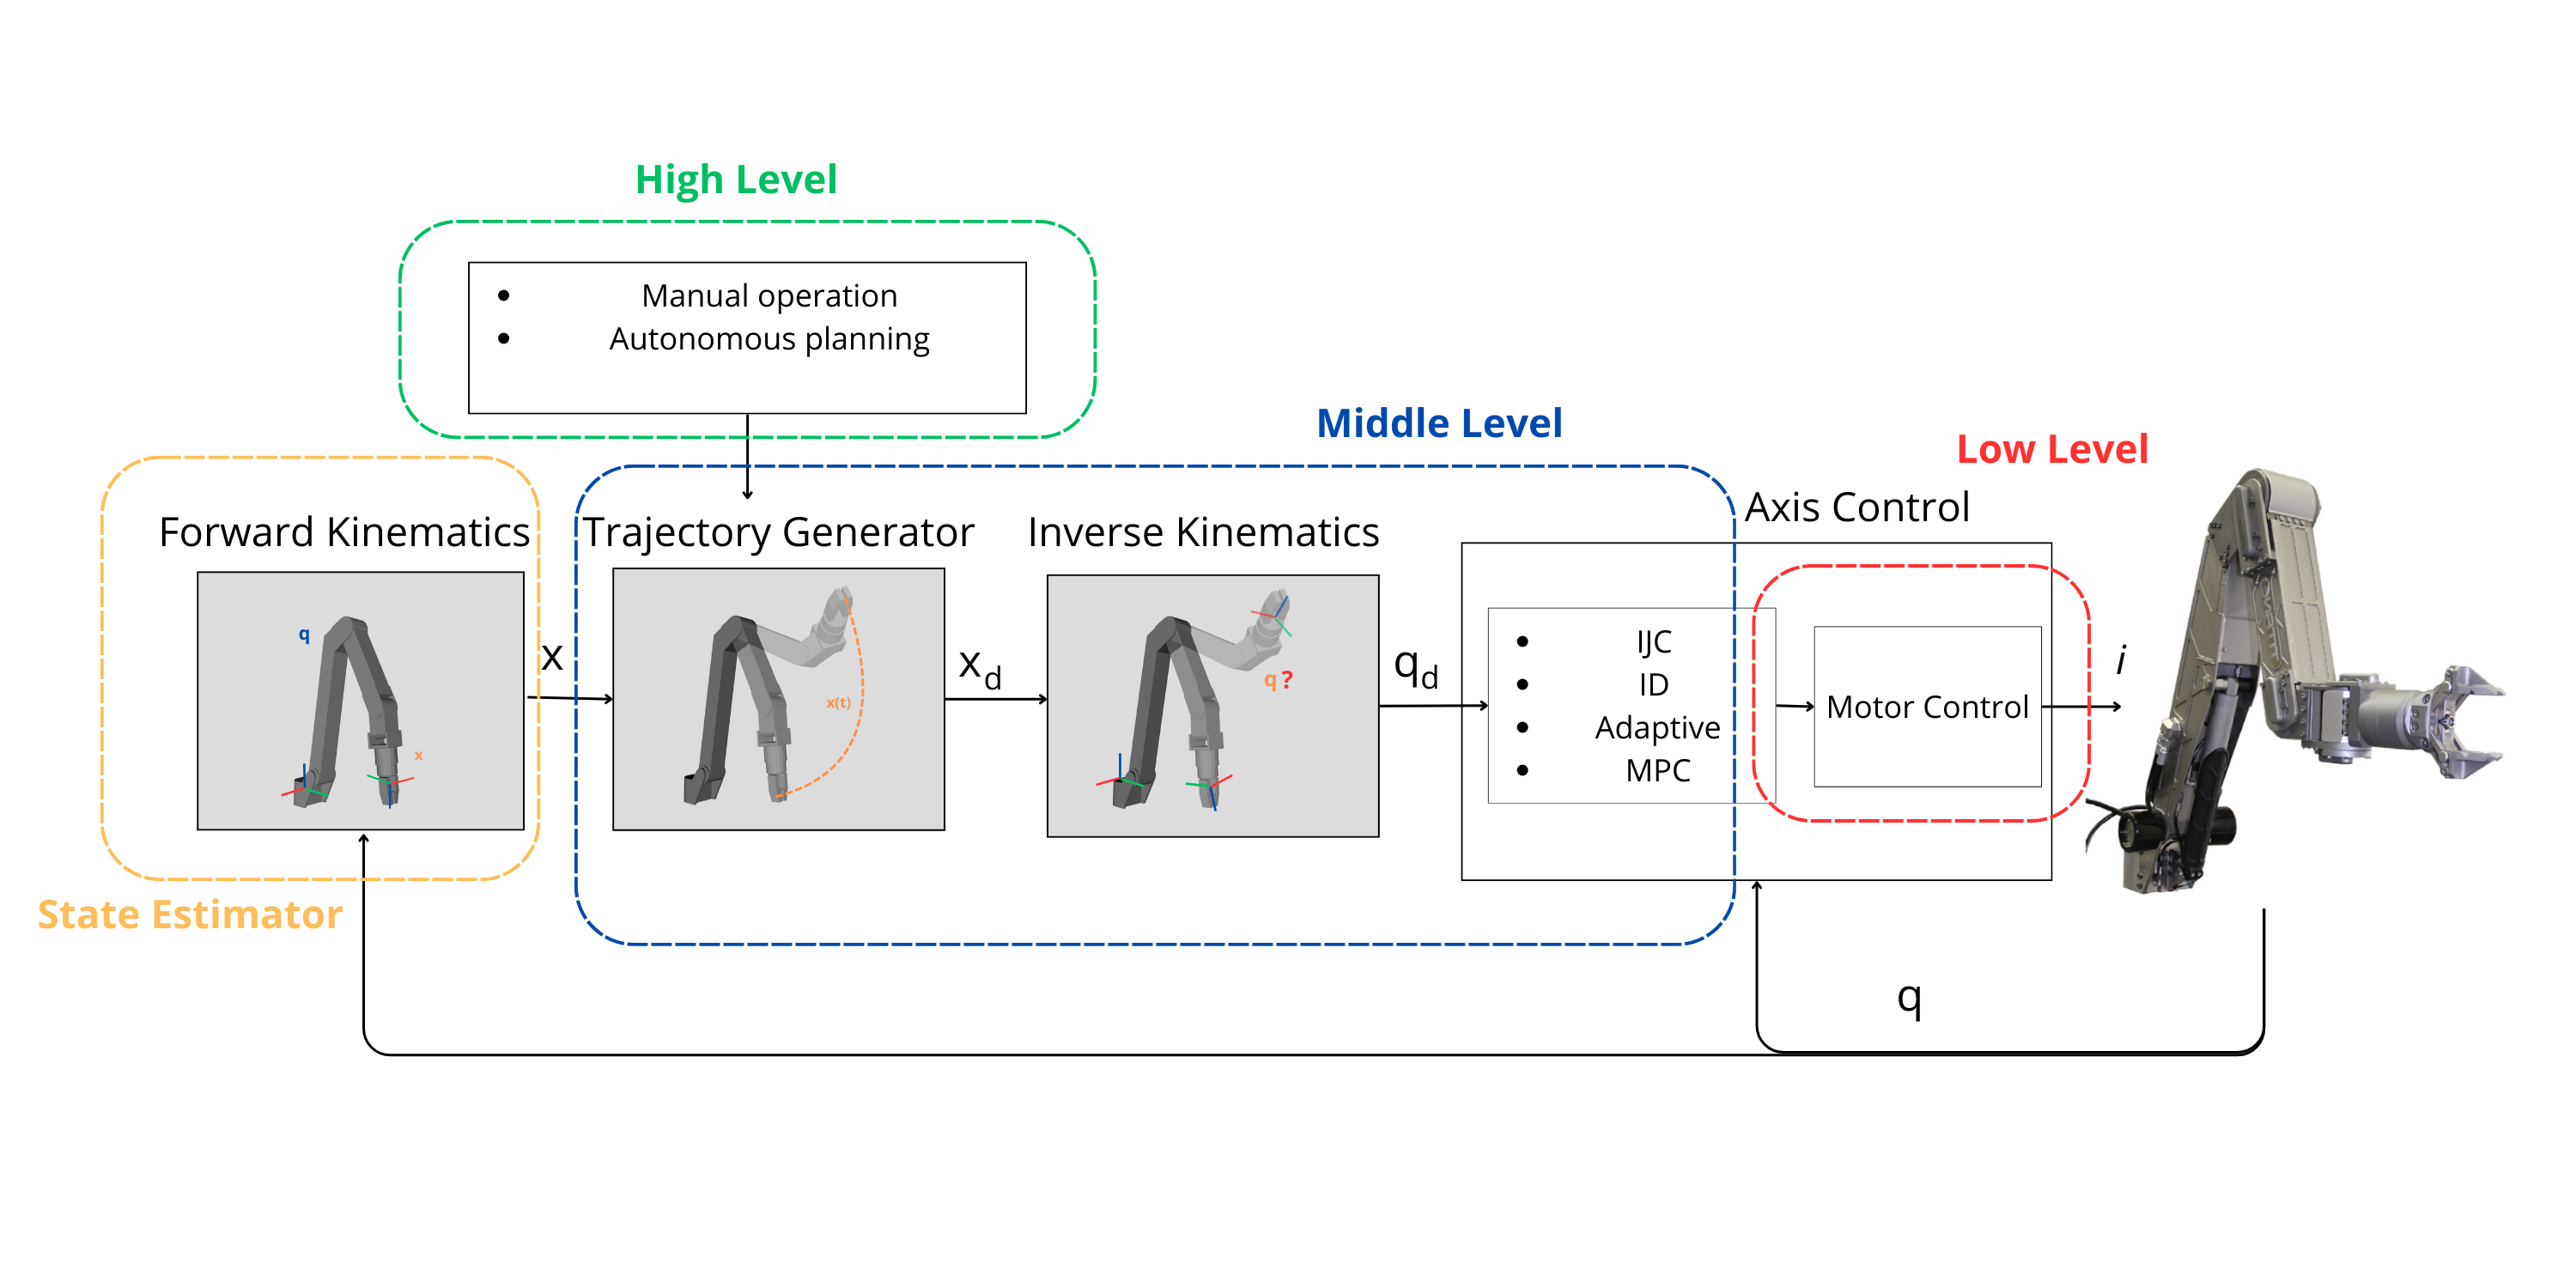
\includegraphics[width=1.1\textwidth]{Images/img_ch2/ManipulatorSchemeControl.png}
    \caption{Schematic representation of manipulator control architecture  }
    \label{fig:ManipulatorControlScheme}
\end{figure}

The IJC is a simple approach to controlling robot motion, for this reason, it is often used in robot prototypes. 

\newpage 
\subsubsection{Indipendent Joint Controller}
\label{sec:IndipendentJointControl}
The decoupled joint dynamics described by Eq.\ref{eq:DecoupledManipulatorEoM} is a good starting point for the design of a decentralized closed-loop control system of the whole robot.

In the Laplace domain, the transfer function from torque to position of each joint motor is:
\begin{equation}
    \label{eq:DecoupledManipulatorEoM}
    G_i(s) = \frac{q_{mi}(s)}{\tau_{mi}(s)} = \frac{\frac{1}{J_{mi} + \frac{J_{li}}{n_i^2}}}{s^2} \quad i = 1,\dots,n
\end{equation}

The idea behind a decentralized control structure is to control each subsystem (joint motor) independently from the others, as represented in Fig.\ref{fig:IJCScheme} below.

\begin{figure}[H]
    \centering
    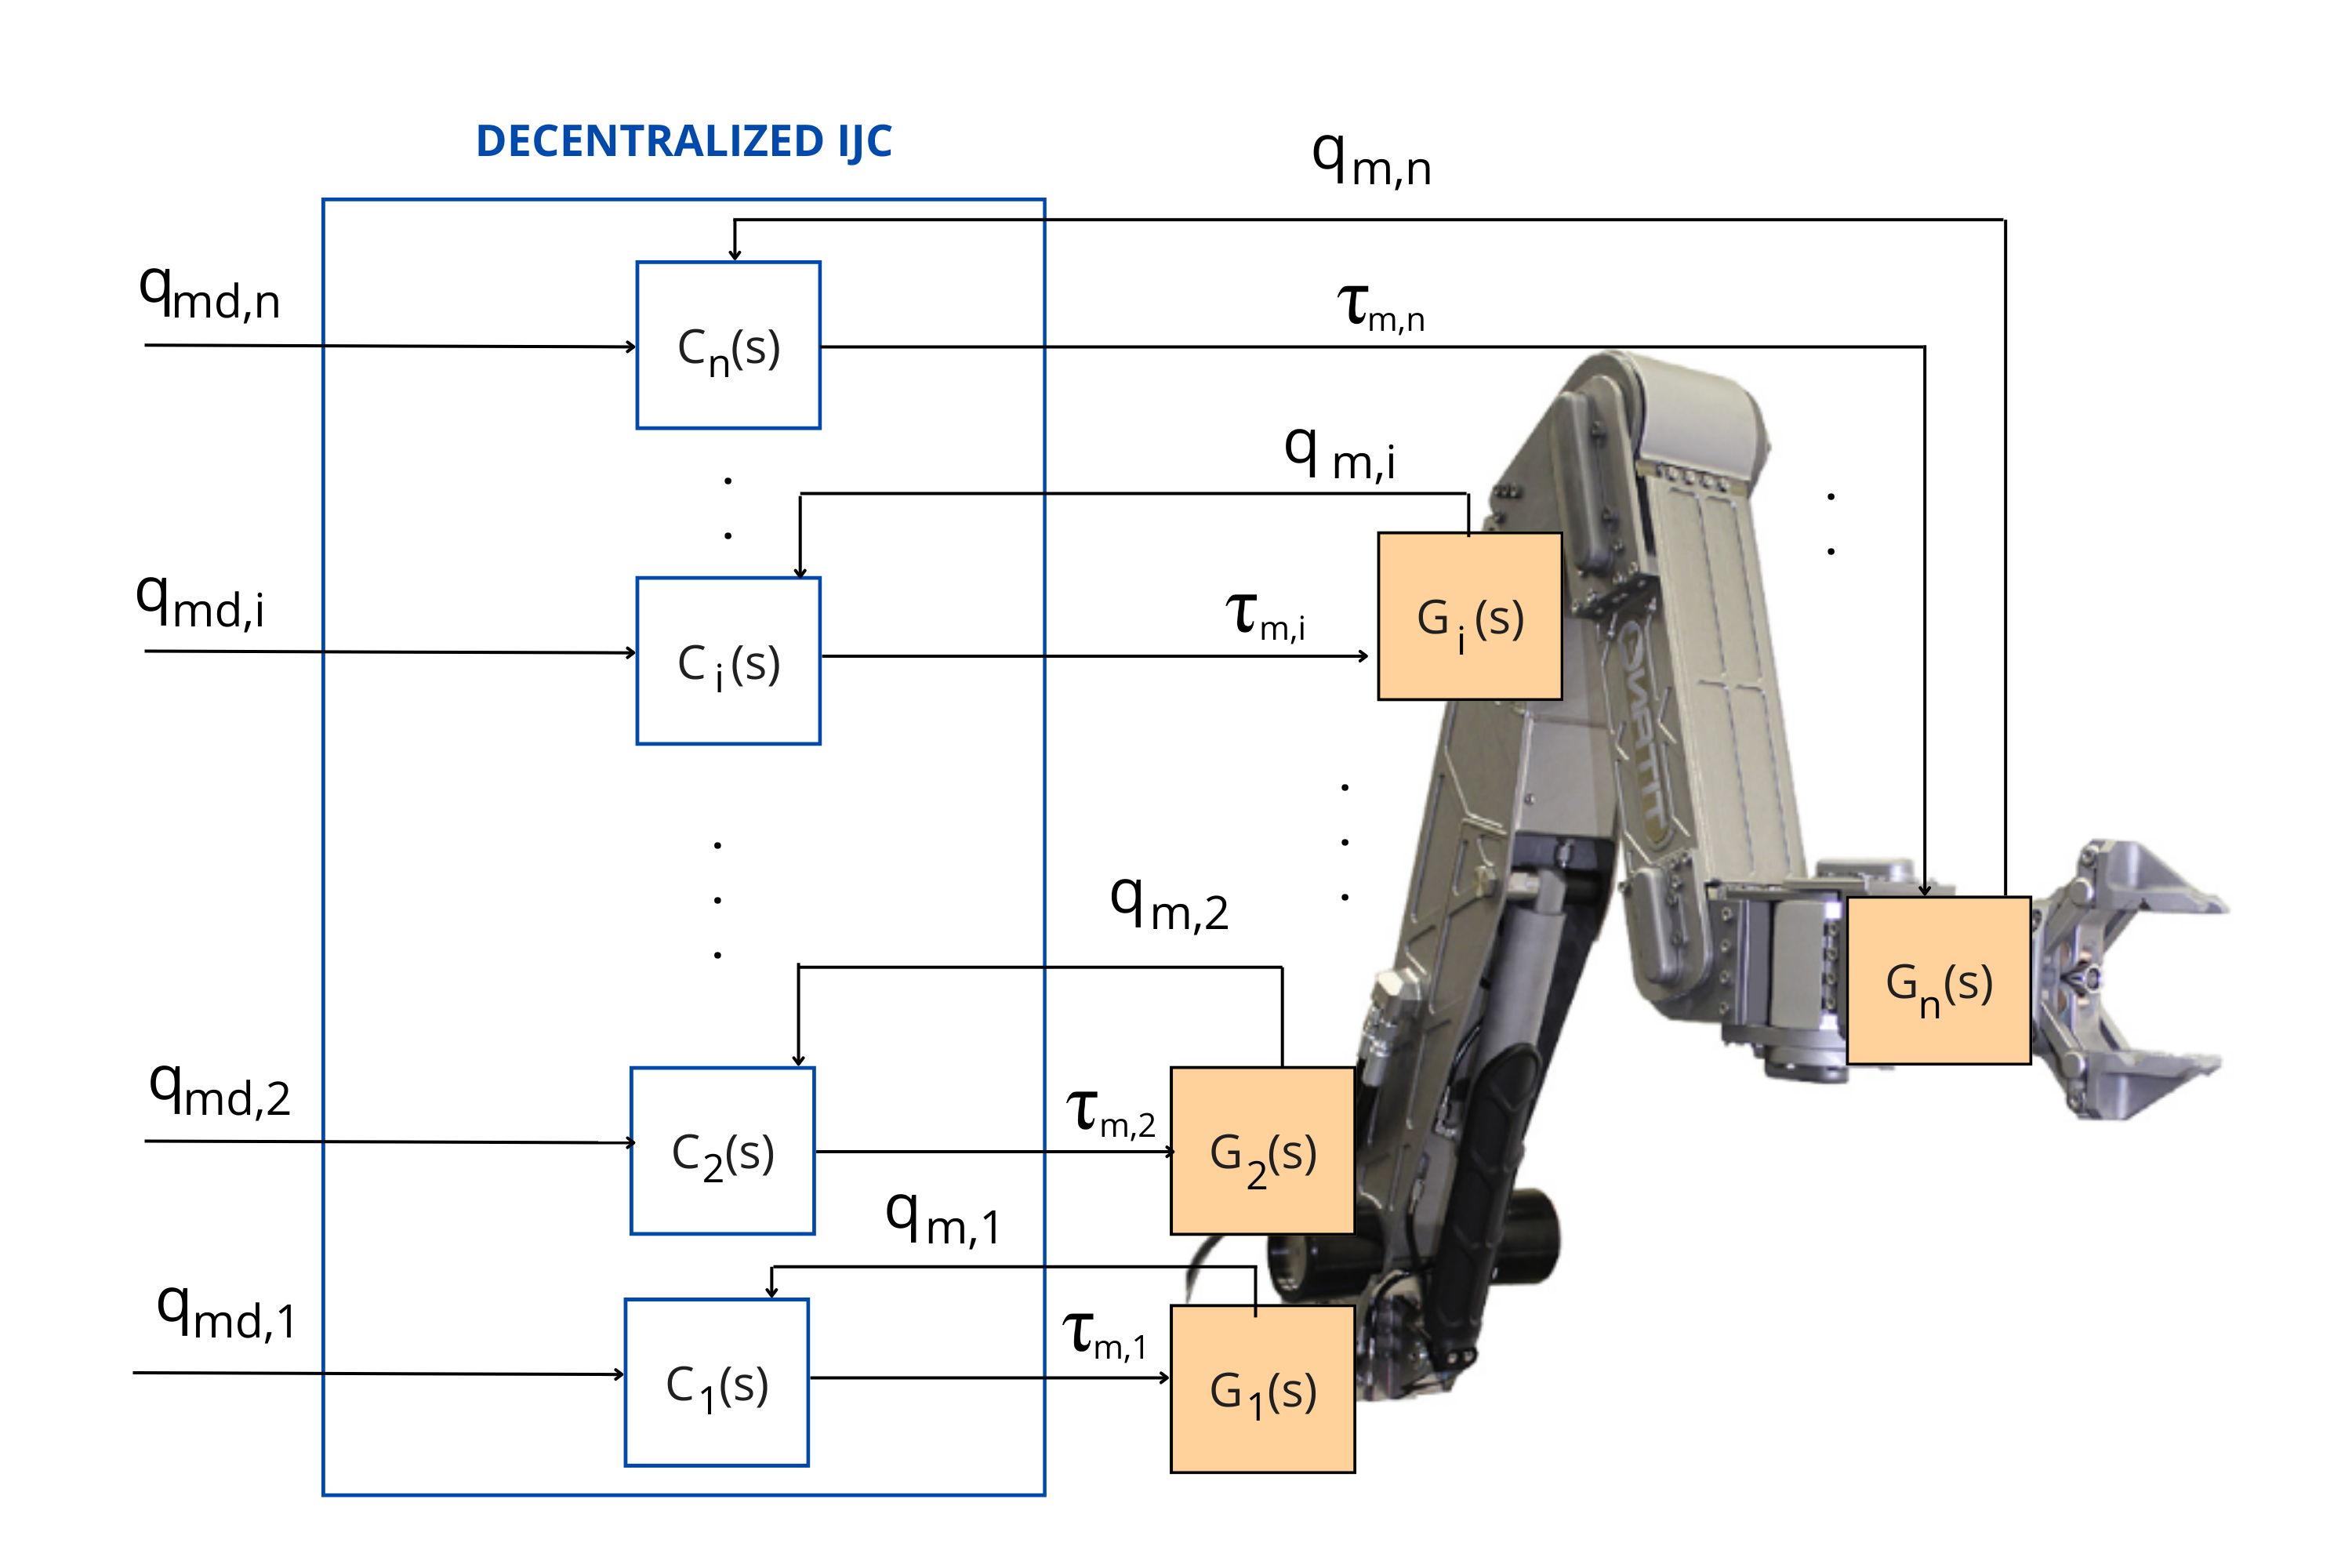
\includegraphics[width=0.7\textwidth]{Images/img_ch2/DecentralizedIJC.png}
    \caption{Schematic representation of a decentralized control structure for a manipulator}
    \label{fig:DecentralizedIJC_Arm}
\end{figure}


Fig.\ref{fig:PPI_IJC} represents the structure of each controller. The motor joint position is often controlled using a cascade controller structure(P+PI), with a proportional(P) in position controller and a proportional-integral(PI) in velocity, and a feed-forward velocity compensation, the controllers are properly tuned accordingly to the system requirements\cite{ControlTheory}.

\begin{figure}[H]
    \centering
    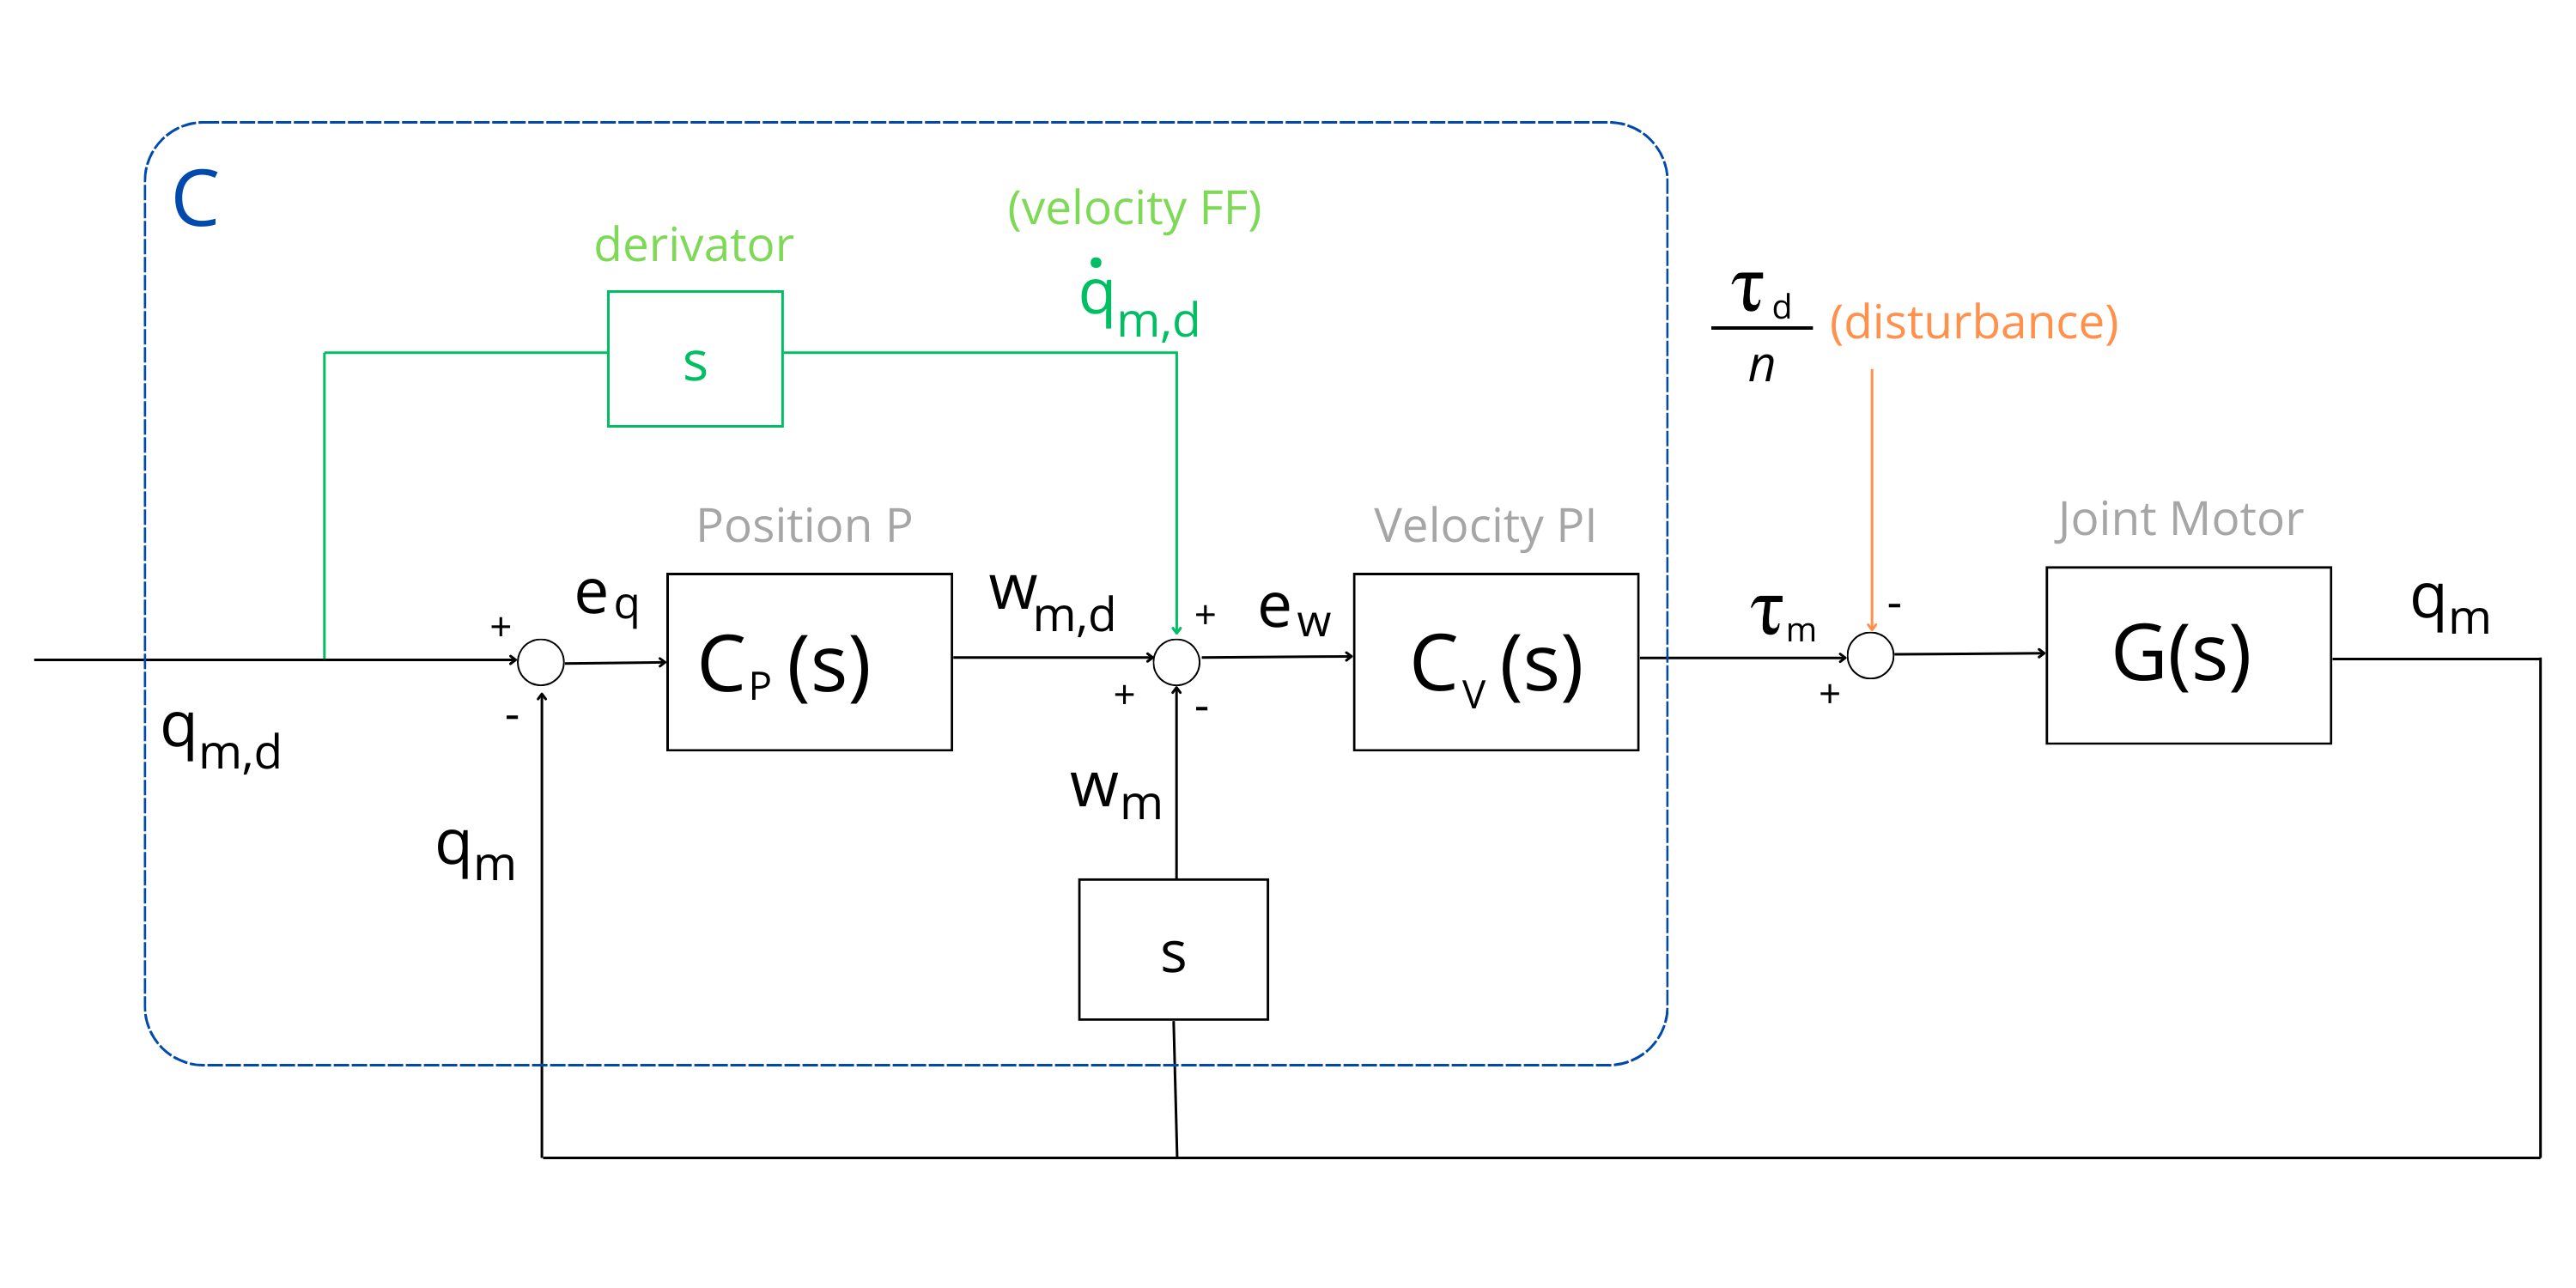
\includegraphics[width=0.7\textwidth]{Images/img_ch2/PPI_IJC.png}
    \caption{Block scheme of P+PI controller of each joint motor}
    \label{fig:PPI_IJC}
\end{figure}

Where the controllers have the following expressions in the Laplace domain: 

$C_P(s) = k_{pp}$ \quad $C_V(s) = k_{pv}\frac{1 + sT_{iv}}{sT_{iv}}$

\subsection{Legged Robots, Walking Machines}
\label{sec:leggedControl}

Legged robots introduce additional levels of complexity to the problem of motion control.
A set of base positions in space defines the motion task, to be executed with a chosen gait without falling or colliding with obstacles.
First of all, common for all mobile robots, the ability to move the base in the environment introduces a higher level of freedom, requiring a further ramification of control: 
\begin{itemize}
    \setlength\itemsep{-0.7em} 
    \item \textbf{Global planning/control}: long-term decision component, works with low frequency to define the trajectory from an initial point to a destination\cite{LeggedPlanning1}. This introduces the additional problem of understanding the environment through localization and mapping algorithms \cite{LeggedLocalization}\cite{AnymalDocThesis}.
    \item \textbf{Local planning/control}: ensure the execution of the global plan, working with high frequency. In legged robots, some of its main components are: gait scheduler, body trajectory control, and leg control (these elements are discussed in the next).  
\end{itemize}
In manipulators, the global planner is the high-level task generator, while the local planner is the architecture below that moves the robot.

Differently from wheeled robots, legged robots' motion is intrinsically discrete, with the advantage of higher traversability capabilities. 
But as introduced in chapter \ref{ch:chapter_one}, legs bring advantages but additional problems, such as base stability. Details on the techniques to evaluate stable conditions for the base position are discussed in chapter \ref{ch:chapter_three}. Intuitively, any legged system, including humans and animals, respects some configuration conditions to avoid falling, due to gravity and other inertial effect. For this reason, during motion, legs are positioned appropriately to maintain stability, humans and animals do it from a learning process, but machines must be instructed to do it. 

The definition of leg contact points along the trajectory is a complex task achieved by the global planner\cite{LIMBEROTakadaThesis}.
Leg order is decided by the \textbf{gait scheduler}, which generates a sequence of leg motion with a timing order, to move the base in a desired direction \cite{Todd}\cite{HiroseDesignGate}\cite{Raibert}. The \textbf{body trajectory controller} instead, keeps the body position in a stable configuration. 

The higher-level components of this architecture are out of the focus of this research, instead, the different techniques to control leg motion from the base specification are discussed now. 

\begin{itemize}
    \setlength\itemsep{-0.7em} 
    \item \textbf{Whole Body Controller} (WBC): Optimization-based control algorithm. Based on the desired base position and the dynamic model of the system, a constrained optimization problem is solved to compute the torque reference for all legs actuators \cite{AnymalDocThesis}\cite{WBCFocchi}\cite{WBCQuadruped}.
    \item \textbf{Model Predictive Control} (MPC): Similarly to the WBC this is an optimization-based control algorithms, which introduce the concept of receding horizon in its "Predictive" feature.  
    \item \textbf{Inverse Dynamic Torque-Based control} (IDC): Similarly to the ID control for manipulators, it is based on the ID problem for legged robots. From the Dynamic model inversion and the desired motion, the required joint torques are computed. When controlling motor torque, Impedance/Admittance control of legs is possible \cite{Siciliano}.
    \item \textbf{Inverse Kinematic Joint control} (IKJC): From the desired base motion, base IK is computed, obtaining each leg joint state. Then each leg is controlled with one of the techniques discussed for manipulator axis control (decentralized IJC, ID, Adaptive, MPC).
\end{itemize}

WBC, MPC, and IDC account for the whole robot dynamic model, ensuring better terrain adaptability, and performance, but dynamic model identification is usually hard.
In IKJC methods instead, each leg is controlled singularly, this is easy to implement but lacks terrain adaptability and ignores the coupled system dynamics. 

As for manipulators, this set of control problems requires a multi-layered control architecture, one possible control scheme is represented in fig.\ref{fig:LeggedControlScheme} below, respecting the "sense-plan-act philosophy". 
Including estimators for the state of the body, each leg, and the surroundings (map and terrain).

\begin{figure}[H]
    \centering
    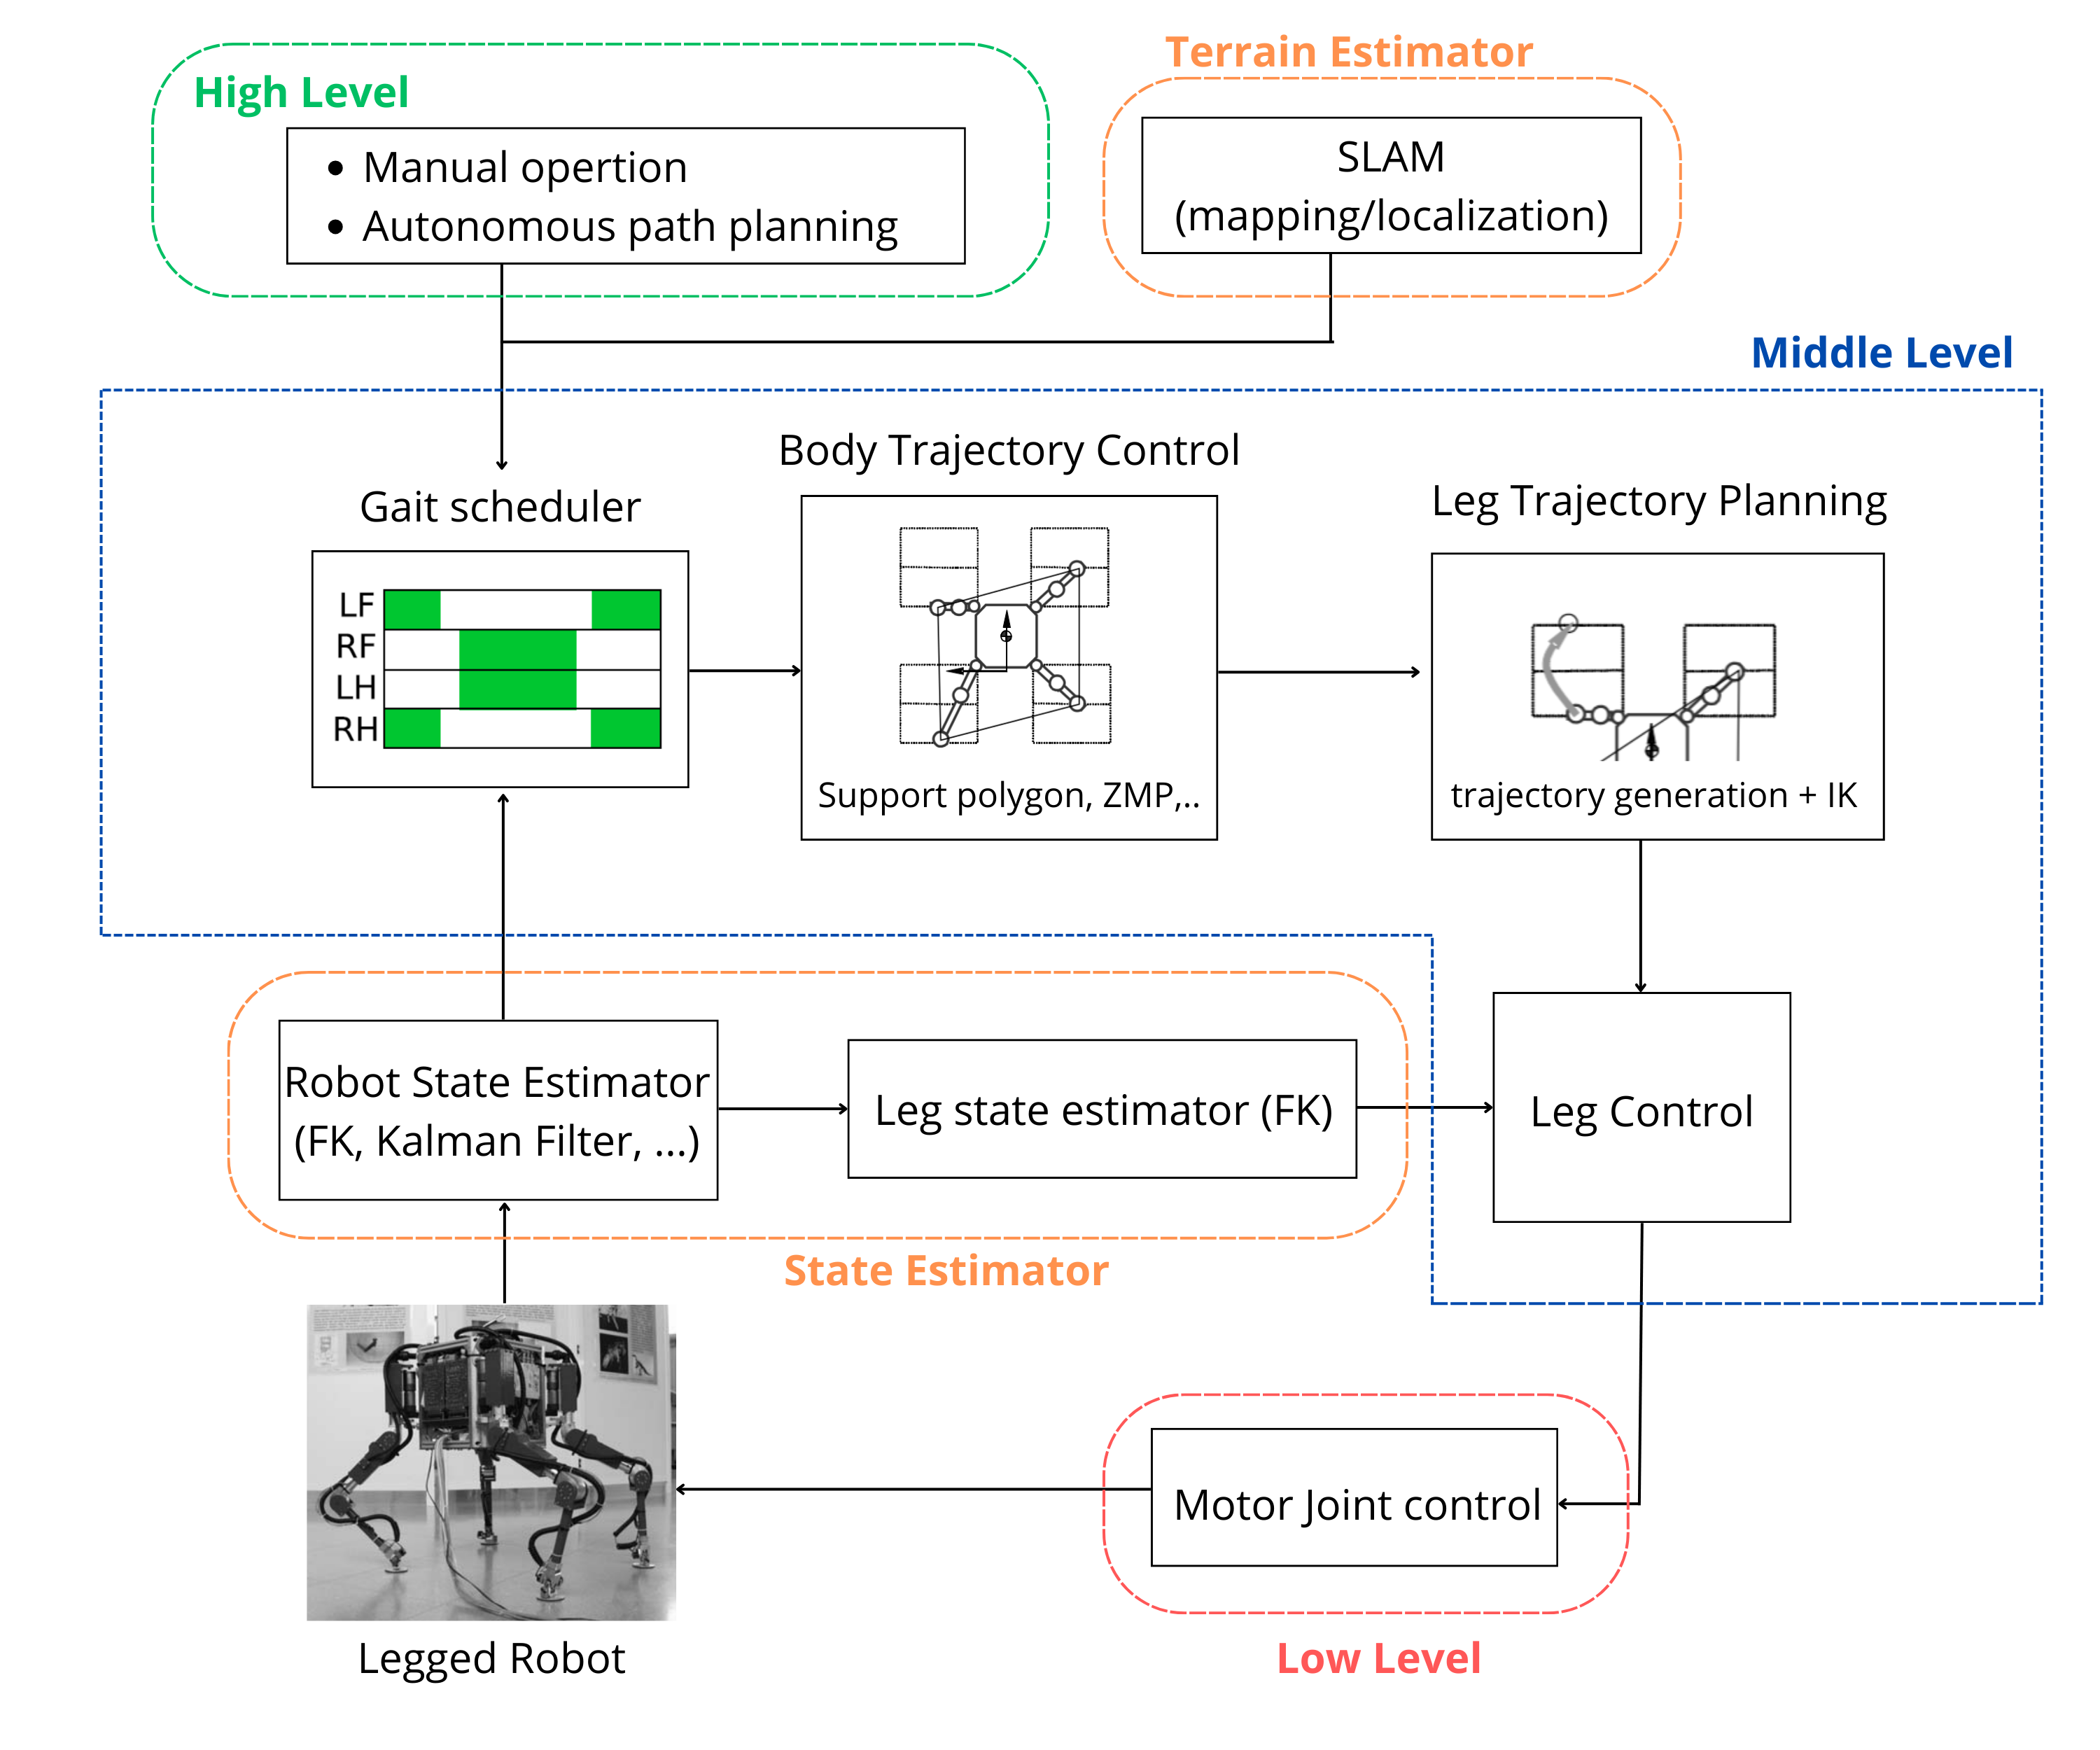
\includegraphics[width=0.8\textwidth]{Images/img_ch2/LeggedControlScheme.png}
    \caption{Schematic representation of one possible legged robot control architecture (some figures are taken from \cite{QuadrupedLocomotion})}
    \label{fig:LeggedControlScheme}
\end{figure}

\subsection{Limbed Robots, Multipurpose Machines}
\label{sec:limbedControl}
Defining a general control structure to control the motion of multi-limbed robots is not possible, due to their multipurpose nature. It is possible to give some task examples: 
\begin{itemize}
    \setlength\itemsep{-0.7em} 
    \item \textbf{Climbing robots}: the motion task is defined by a set of base positions in space (as for walking robot), to be reached while maintaining wall/ceiling adhesion and without colliding with obstacles\cite{KentaroUnoPhD}.
    \item \textbf{Walking/Climbing + Manipulating robots}: When limbs are designed also to manipulate objects in the environment. That means that tasks can be of two natures, reaching positions in space or moving limb tip in a sequence of positions, sometimes at the same time (walking while manipulating).
    \item \textbf{Driving + Walking robots}: legged-wheeled robots\cite{AnymalDocThesis}\cite{WheelLeggedStabilityOPT} add the additional legs DOF to the classical wheeled locomotion, making possible hybrid locomotion (like skating). The task is reaching poses in space, but additional decisional problems arise. 
    \item \textbf{Hybrid robots}: For robots equipped with transformable EE at limb tips, the complexity of modeling and control increases. Walking, climbing, driving, and manipulating tasks are unlocked. 
\end{itemize}

While walking machines are constrained to stay on the ground, space multi-limbed robots move around gripping the surroundings \cite{Ribeiro2023reaction}\cite{RibeiroGroundGripping}\cite{ISSLimbedRobot}. 
Professor Oussama Khatib implemented a possible solution to this complex scenario, the "constrained consistent task oriented WBC"\cite{KhatibConstrainedConsistentTaskOrientedWBC}. He defined a task-oriented control algorithm for humanoid robots, that can be generalized to different complex robotic structures.  
The details of this control algorithm are out of the scope of this research.

Another possible simpler solution is to consider again a multi-layered control structure, similar to the one discussed for walking machines (see Fig.\ref{fig:LeggedControlScheme}). In this case, additional complexity is included at a high level, where different types of tasks are generated. 
The output of high-level components will also include the type of task, and at middle-level decisions are taken accordingly. For the limb controller, reliable control algorithms (MPC, WBC, ID) are used to adapt to different tasks, such as moving the base, manipulating a heavy object, or gripping a rocky wall. 
Each module can be implemented using the concepts discussed for manipulators and climbing robots, but care must be taken due to the different tasks and situations addressed by the robot. 

